\chapter{Period-adding in the Archetypal Model}
\label{chap:add}

It was shown that there are period-adding structures in piecewise linear continuous increasing circle maps by \Citeauthor{simpson2018saw}.
He calls these types of functions skew sawtooth maps~\cite{simpson2018saw}.
The archetypal model function is not continuous, has four branches instead of two, and only linear on two of four branches.
But it is also a circle map, \gls{pws}, and mostly increasing.
\Cref{fig:add.saw.vs.arch} shows both maps for comparison.
In this chapter, we modify the fixed parameters of the archetypal model to produce period-adding structures.
The idea is to make the archetypal model function as similar as possible to a skew sawtooth map.

\begin{figure}
	\centering
	\subfloat[Skew sawtooth map]{
		\includegraphics[width=.45 \textwidth]{81_Sawtooth/Sketch/result.png}
		\label{fig:add.saw}
	}
	\subfloat[Archetypal model function]{
		\includegraphics[width=.45 \textwidth]{60_MinimalRepr/Sketch/result.png}
		\label{fig:add.arch}
	}
	\caption[Comparison of a skew sawtooth map and the archetypal model function]{
		Comparison of a skew sawtooth map and the archetypal model function.
		(a) shows the skew sawtooth map with the parameters $a_L = 0.5$ and $a_R = 1.5$.
		The function is taken from \Citetitle{simpson2018saw}~\cite{simpson2018saw}.
		(b) shows the archetypal model function with the parameters $a_L = 4, b_L = -\frac{1}{2}, c_L = 0.168, g_R\left(\frac{1}{4}\right) = -0.4 ,$ and $g_R\left(\frac{1}{2}\right) = \frac{1}{2} + \frac{1}{40}$.
	}
	\label{fig:add.saw.vs.arch}
\end{figure}

\section{Adjusting the Parameters}
\label{sec:add.parameters}

\hl{
	The fixed parameters in the archetypal are $a_L = 4, b_L = -\frac{1}{2},$ and $g_R\left(\frac{1}{2}\right) = \frac{1}{2} + \frac{1}{40}$.
	\hl{O}nly the branches $f_\A$ and $f_\C$ are not monotonously increasing.
	Of the three fixed parameters, $a_L$ and $b_L$ influence the shape of the branches $f_\A$ and $f_\C$.
	These parameters are adjusted to make the branches $f_\A$ and $f_\C$ monotonously increasing.
	The new parameter values are $a_L = 1$ and $b_L = \frac{1}{2}$.
}
\hl{The new shape of the function can be seen in} \Cref{fig:add.arch.new}, \hl{now all branches are monotonously increasing}.
\hl{
	We will refer to this model as the piecewise-increasing archetypal model.
}

\Cref{fig:add.arch.new.period} \hl{shows a 2D scan of the periods associated with parameter regions in the archetypal model with these new values for the fixed parameters stated above}.
\hl{
	In this scan, we can see that the ``type B'' parameter regions disappeared and ``type A'' parameter regions of the same chain seem to start overlapping.
	Also, in between the chains there are now small parameter regions with much higher periods.
	These structures look like \glsentrylong{pa} structures.
	And indeed, it is plausible for \gls{pa} structures to emerge in such a map.
	\Citeauthor{simpson2018saw} demonstrated in his work \cite{simpson2018saw} that a \gls{pws} circle map with two linear and increasing branches can exhibit \gls{pa}.
}
\Cref{fig:add.saw} \hl{shows this map called skew sawtooth next to the piecewise-increasing archetypal model map}.
\hl{
	The skew sawtooth map is continuous while the piecewise-increasing archetypal model map is not.
	And the piecewise-increasing archetypal map has quadratic branches while all branches in the skew sawtooth map are linear.
}
\hl{But they are somewhat similar as we can see in the comparison in} \Cref{fig:add.saw.vs.arch}.

\hl{
	In the following sections these structures are explored.
	They are referred to as \gls{pal} structures.
}
But first, we will take a closer look at how the bifurcations structures change when adjusting the parameters $a_L$ and $b_L$ to make the branches $f_\A$ and $f_\C$ increasing.

\begin{figure}
	\centering
	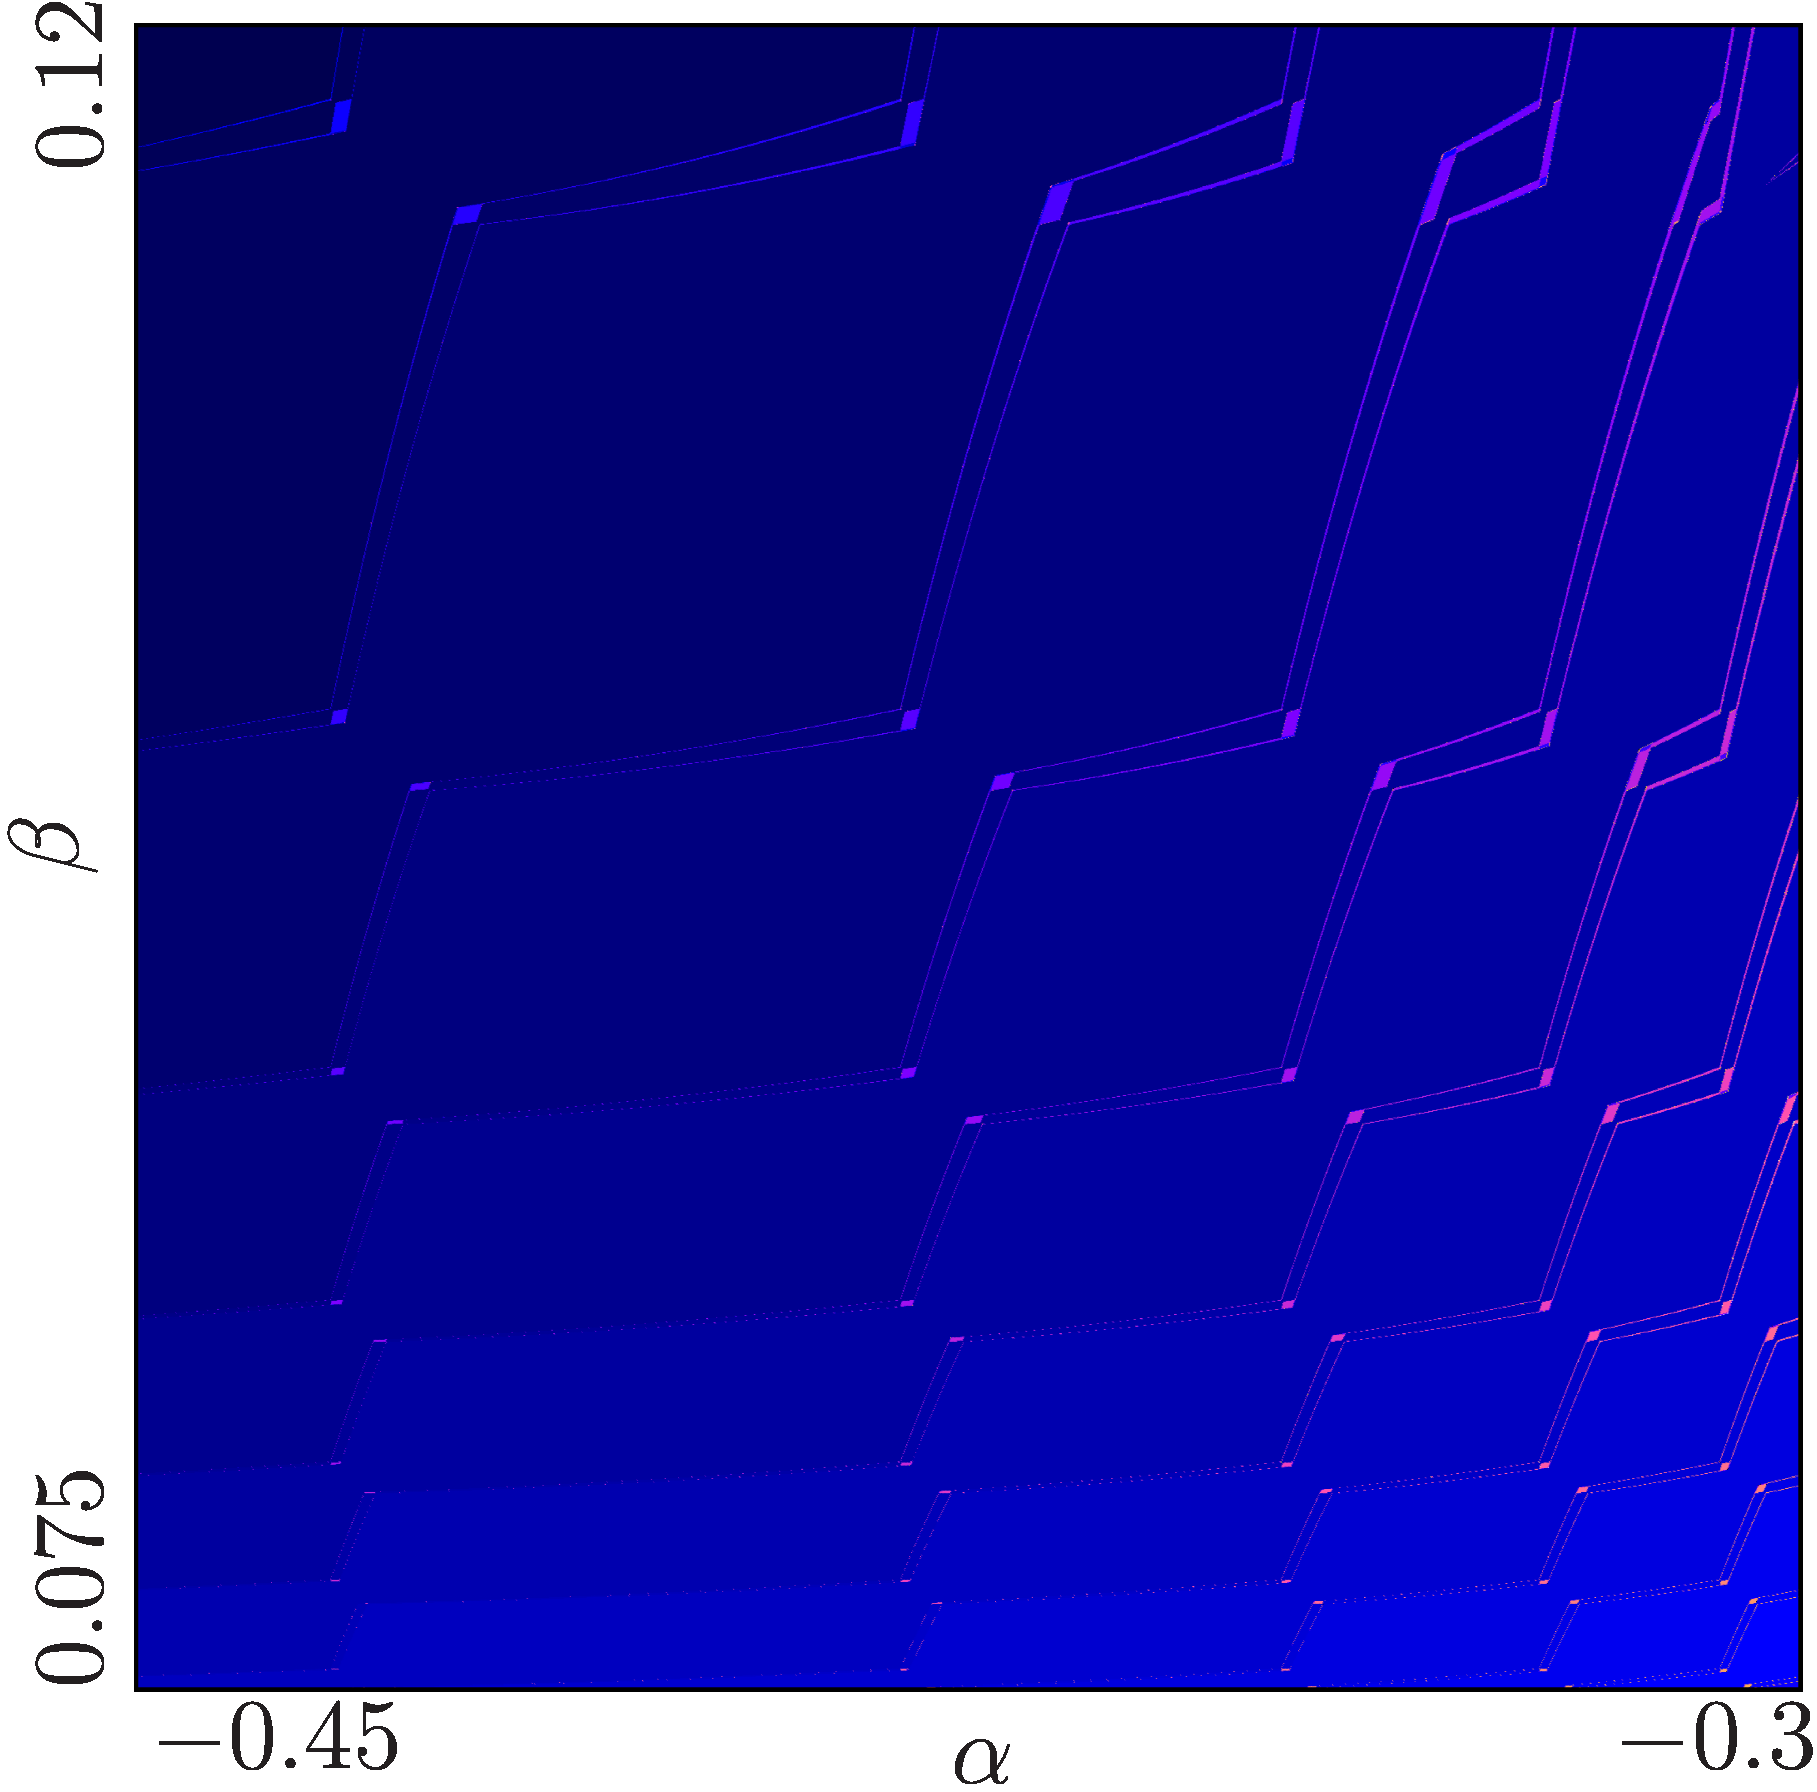
\includegraphics[width=.6 \textwidth]{../Figures/7/7.1/result.png}
	\caption[2D period scan of the piecewise-increasing increasing archetypal model]{
		2D period scan of the piecewise-increasing increasing archetypal model.
		With the fixed parameters $a_L = 1, b_L = \frac{1}{2},$ and $g_R\left(\frac{1}{2}\right) = \frac{1}{2} + \frac{1}{40}$.
		The parameters $\alpha = g_R\left(\frac{1}{4}\right)$ and $\beta = c_L$ are varied.
	}
	\label{fig:add.arch.new.period}
\end{figure}

\begin{figure}
	\centering
	\subfloat[Skew sawtooth map]{
		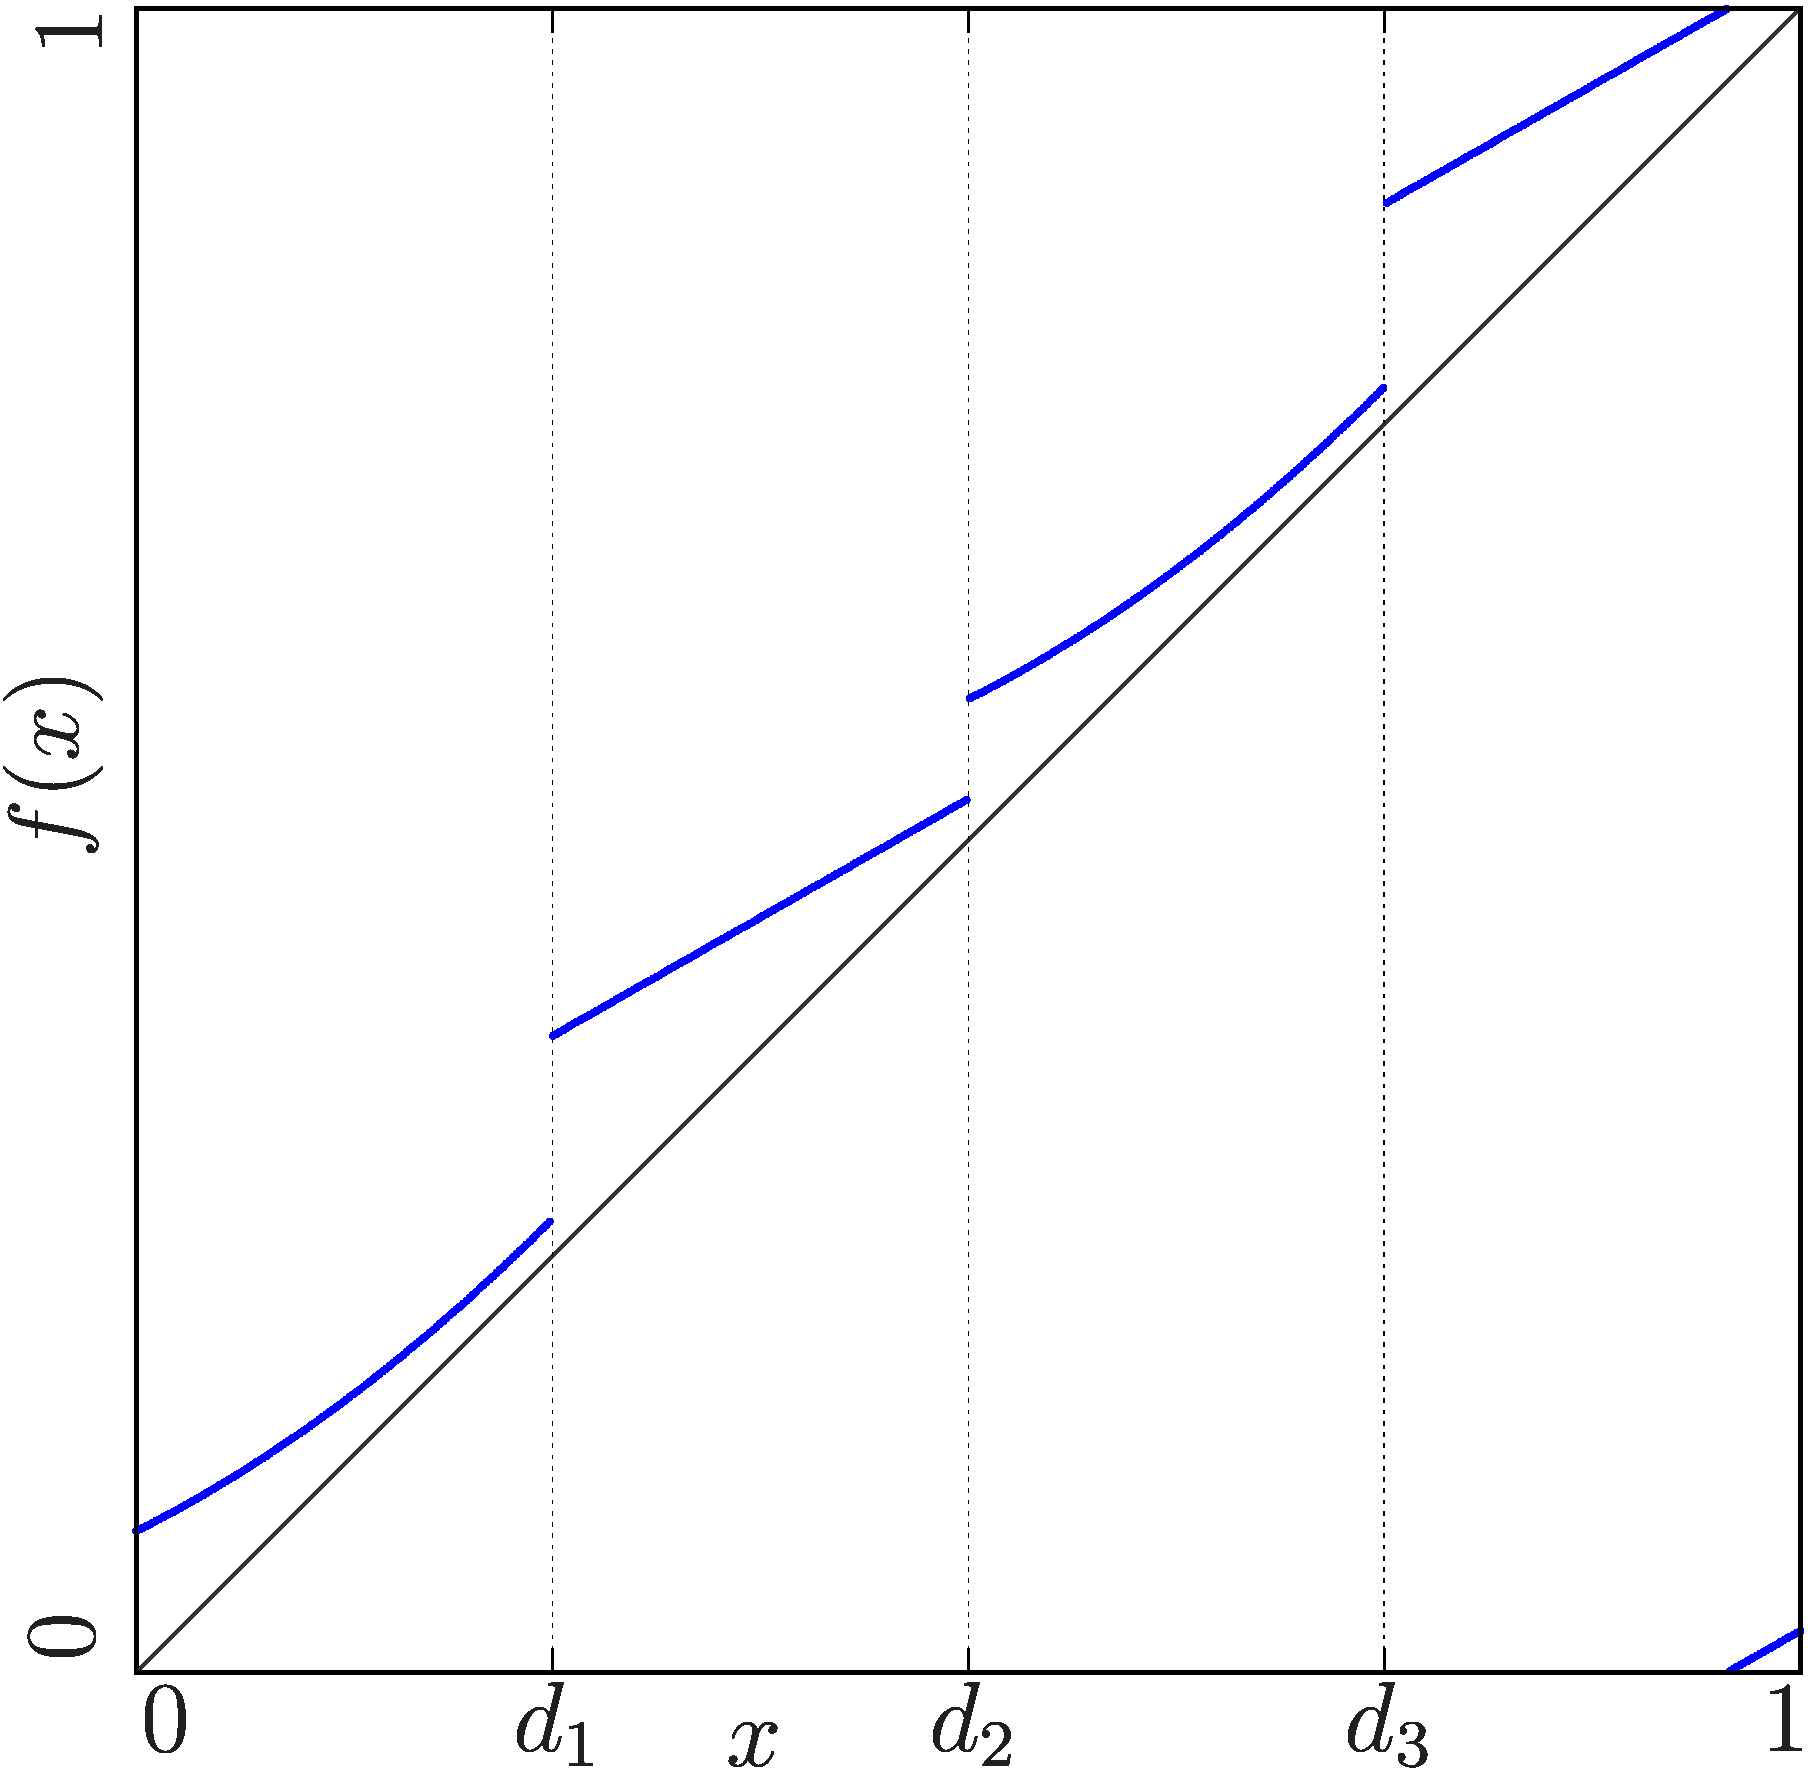
\includegraphics[width=.4 \textwidth]{../Figures/7/7.2a/result.png}
		\label{fig:add.saw}
	}
	\subfloat[Function shape]{
		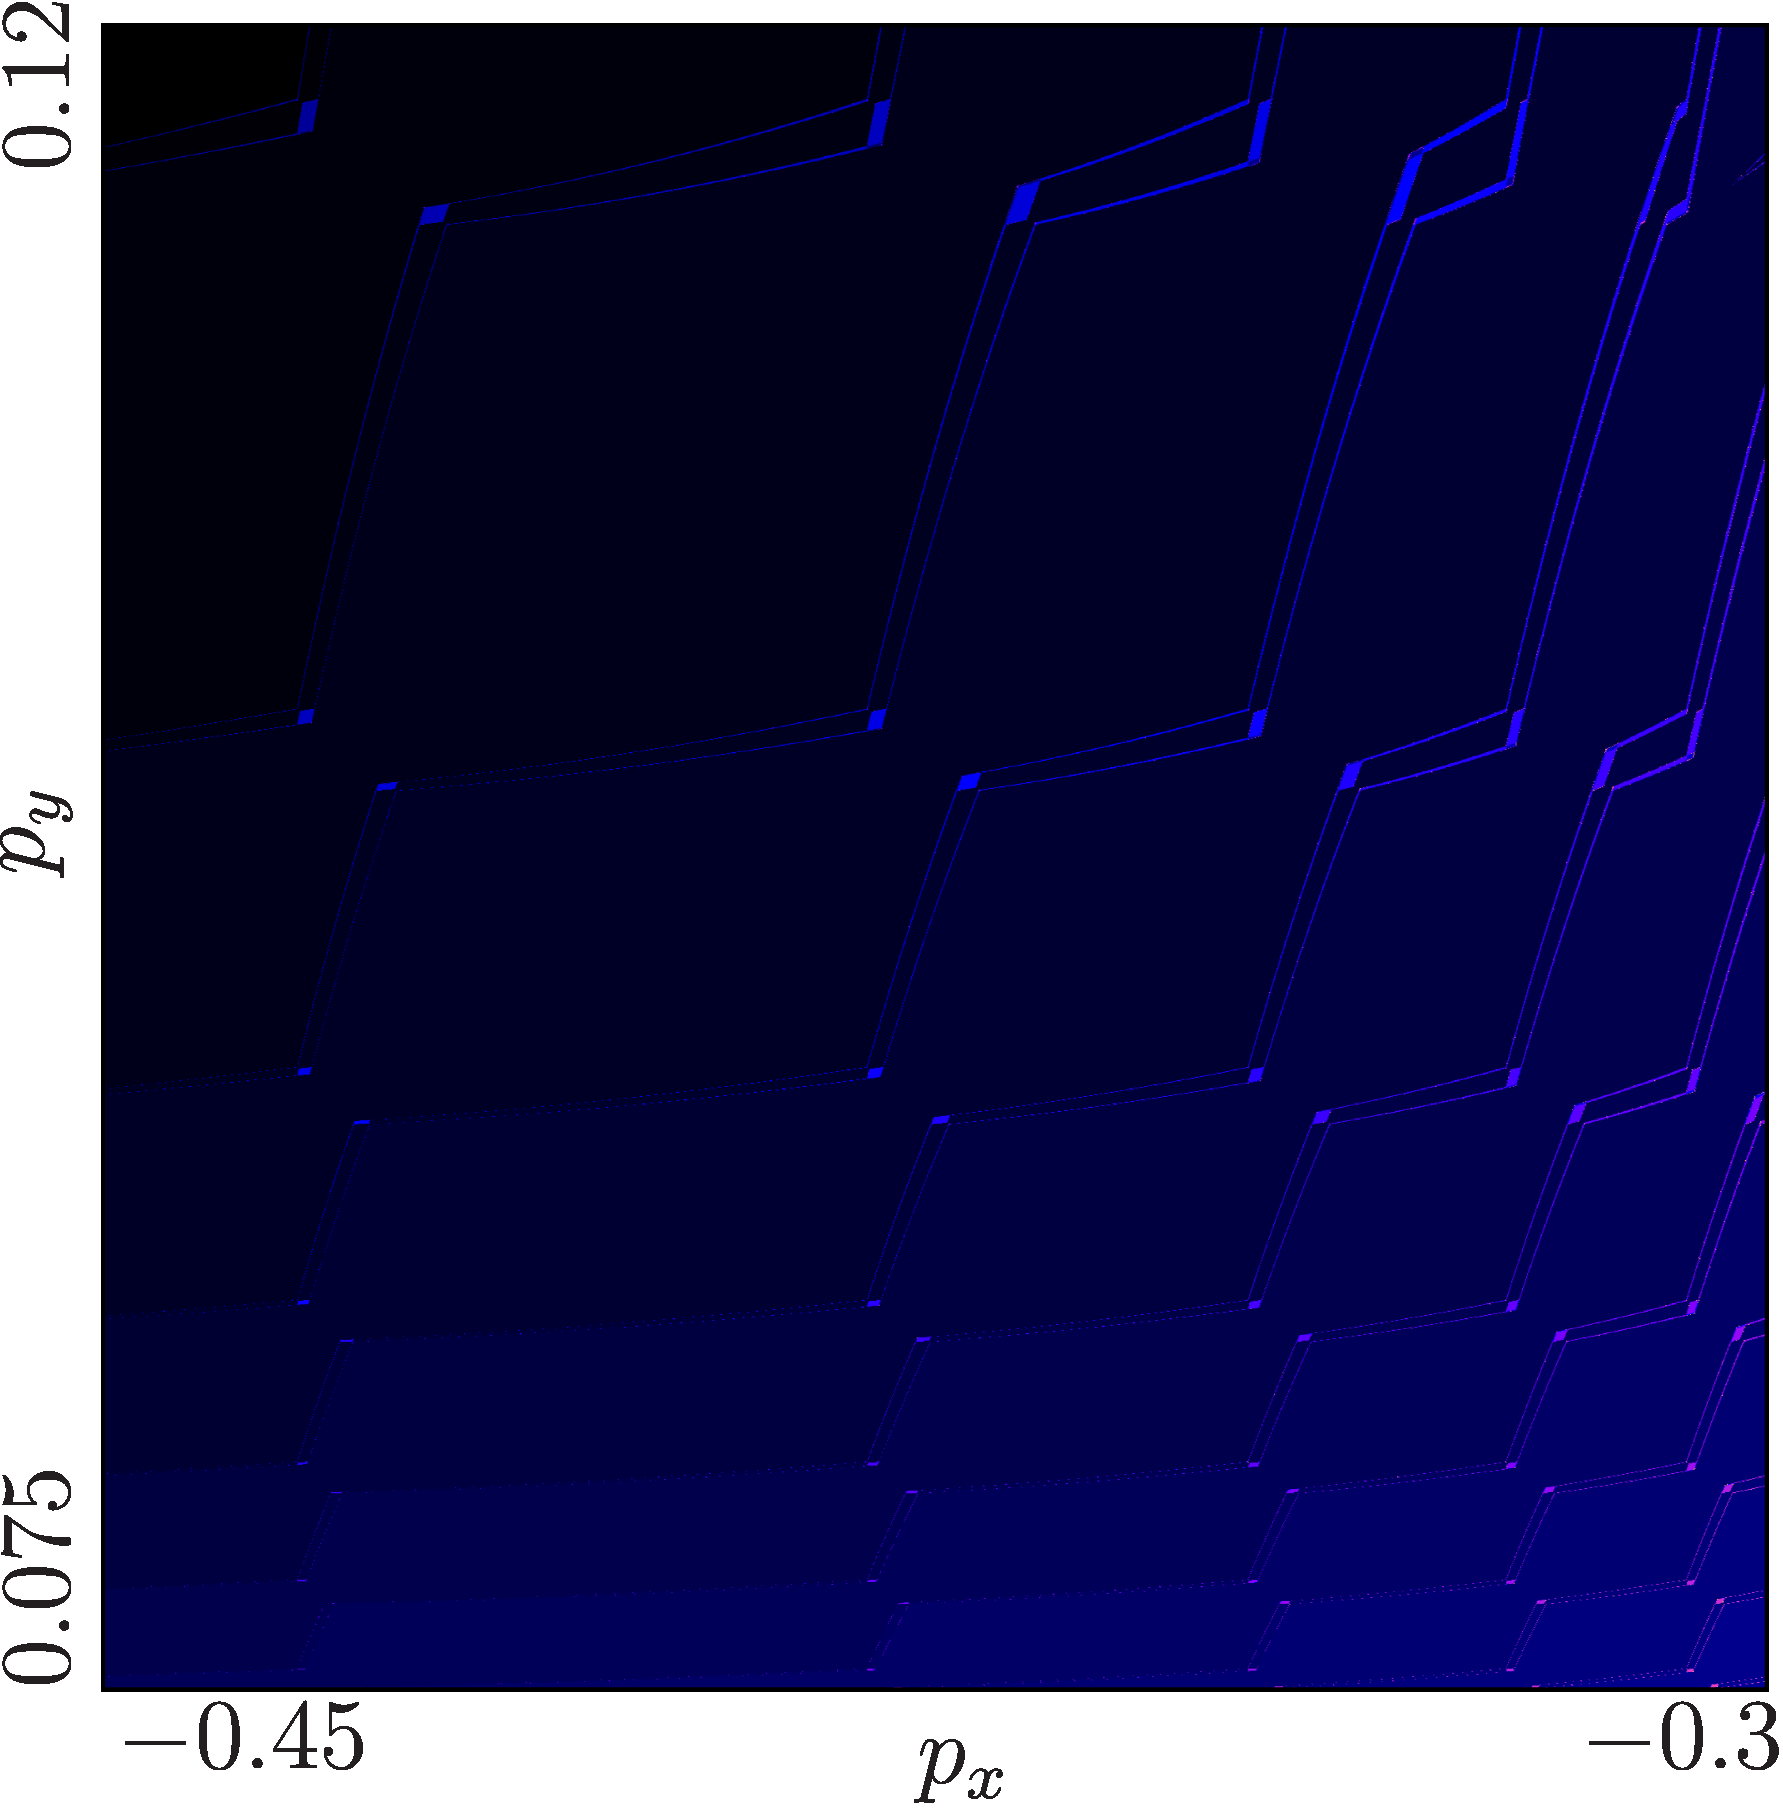
\includegraphics[width=.4 \textwidth]{../Figures/7/7.2b/result.png}
		\label{fig:add.arch.new}
	}
	\caption[Comparison of the piecewise-increasing archetypal model function and the skew sawtooth map]{
		Comparison of the piecewise-increasing archetypal model function and the skew sawtooth map.
		(a) shows the archetypal model function with the parameters $a_L = 1, b_L = \frac{1}{2}, c_L = 0.168, g_R\left(\frac{1}{4}\right) = -0.4 ,$ and $g_R\left(\frac{1}{2}\right) = \frac{1}{2} + \frac{1}{40}$.
		(b) shows the skew sawtooth map \hl{which is defined in} \cite{simpson2018saw} with the parameters $a_L = 0.5$ and $a_R = 1.5$.
		The parameters happen to have similar names to the parameters of the archetypal model.
	}
	\label{fig:add.saw.vs.arch}
\end{figure}

\section{Changes to the Bifurcation Structure}
\label{sec:add.change}

This section examines how changing the parameters as described in \Cref{sec:add.parameters} changes the bifurcation structure of the archetypal model.

\subsection{Numerical Overview of the Changes to the Bifurcation Structure}
\label{sec:add.change.num}

\Cref{fig:add.change.regions} shows diagrams depicting the borders of parameter regions with different symbolic sequences.
These diagrams are used as the basis for the exploration of changes to the bifurcation structure.
The lower left corner of the diagrams is always in the period region with the stable cycle $\Cycle{\A^7\B^3\C^7\D^3}$.
The cycles in the upper left ($\Cycle{\A^6\B^3\C^6\D^3}$), upper right ($\Cycle{\A^6\B^4\C^6\D^4}$), lower right ($\Cycle{\A^7\B^4\C^7\D^4}$), and middle ($\Cycle{\A^7\B^3\C^6\D^4}$ and $\Cycle{\A^6\B^4\C^7\D^3}$) follow.

Here, a short notation for the symbolic sequences is introduced.
``Type A'' parameter regions where the cycle is associated with the symbolic sequence $\A^a\B^b\C^a\D^b$ are written as $P^{2 \cdot \left(a + b\right)}_b$
``Type B'' parameter regions where the coexisting twin cycles are associated with the symbolic sequences $\A^a\B^b\C^c\D^d$ and $\A^c\B^d\C^a\D^b$ where $c = a - 1$ and $d = b + 1$ are written as $P^{a + b + c + d}_b$.
So for example, the ``type A'' parameter region in the lower left corner of every diagram in \Cref{fig:add.change.regions} is written as $P^{20}_3$.

There is also a new type of parameter region that we call hybrid parameter regions with hybrid cycles.
Hybrid cycles are cycles that are asymmetrical like ``type B'' cycles and therefore also exist in pairs.
The difference to ``type B'' cycles is that for two hybrid twin cycles with the symbolic sequences $\A^a\B^b\C^c\D^d$ and $\A^c\B^d\C^a\D^b$ either $c \neq a - 1$ or $d \neq b + 1$ but $c \leq a$ and $d \geq b$.
For example, the two hybrid twin cycles $\Cycle{\A^7\B^4\C^6\D^4}$ and $\Cycle{\A^6\B^4\C^7\D^4}$.
Their corresponding parameter region is written  in the short notation.
The short notation for their corresponding parameter regions is $P^{22}_4$ and $P^{20}_4$, respectively.
The parameter region with such hybrid cycles is written as $\left[P^{22}_4 \mid P^{20}_4\right]$.
This notation is chosen because of an operation that is introduced in the later \Cref{sec:add.add.halved}.
\Cref{sec:add.change.appa} covers how these parameter regions are created.
These parameter regions are connected to the \gls{pal} structures next to them, as we will see later in \Cref{sec:add.add.halved}.

The four different diagrams in \Cref{fig:add.change.regions} show the evolution at different points during the transition from the archetypal model to the piecewise-increasing archetypal model.
For this, the parameter values for $a_L$ and $b_L$ are chosen along a line given by \Cref{equ:add.change.paramline}.
\begin{align}
	a_L = \frac{5}{2} - 3 \cdot b_L
	\label{equ:add.change.paramline}
\end{align}

\begin{figure}
	\centering
	\subfloat[$a_L = 3.5, b_L = -0.\overline{3}$]{
		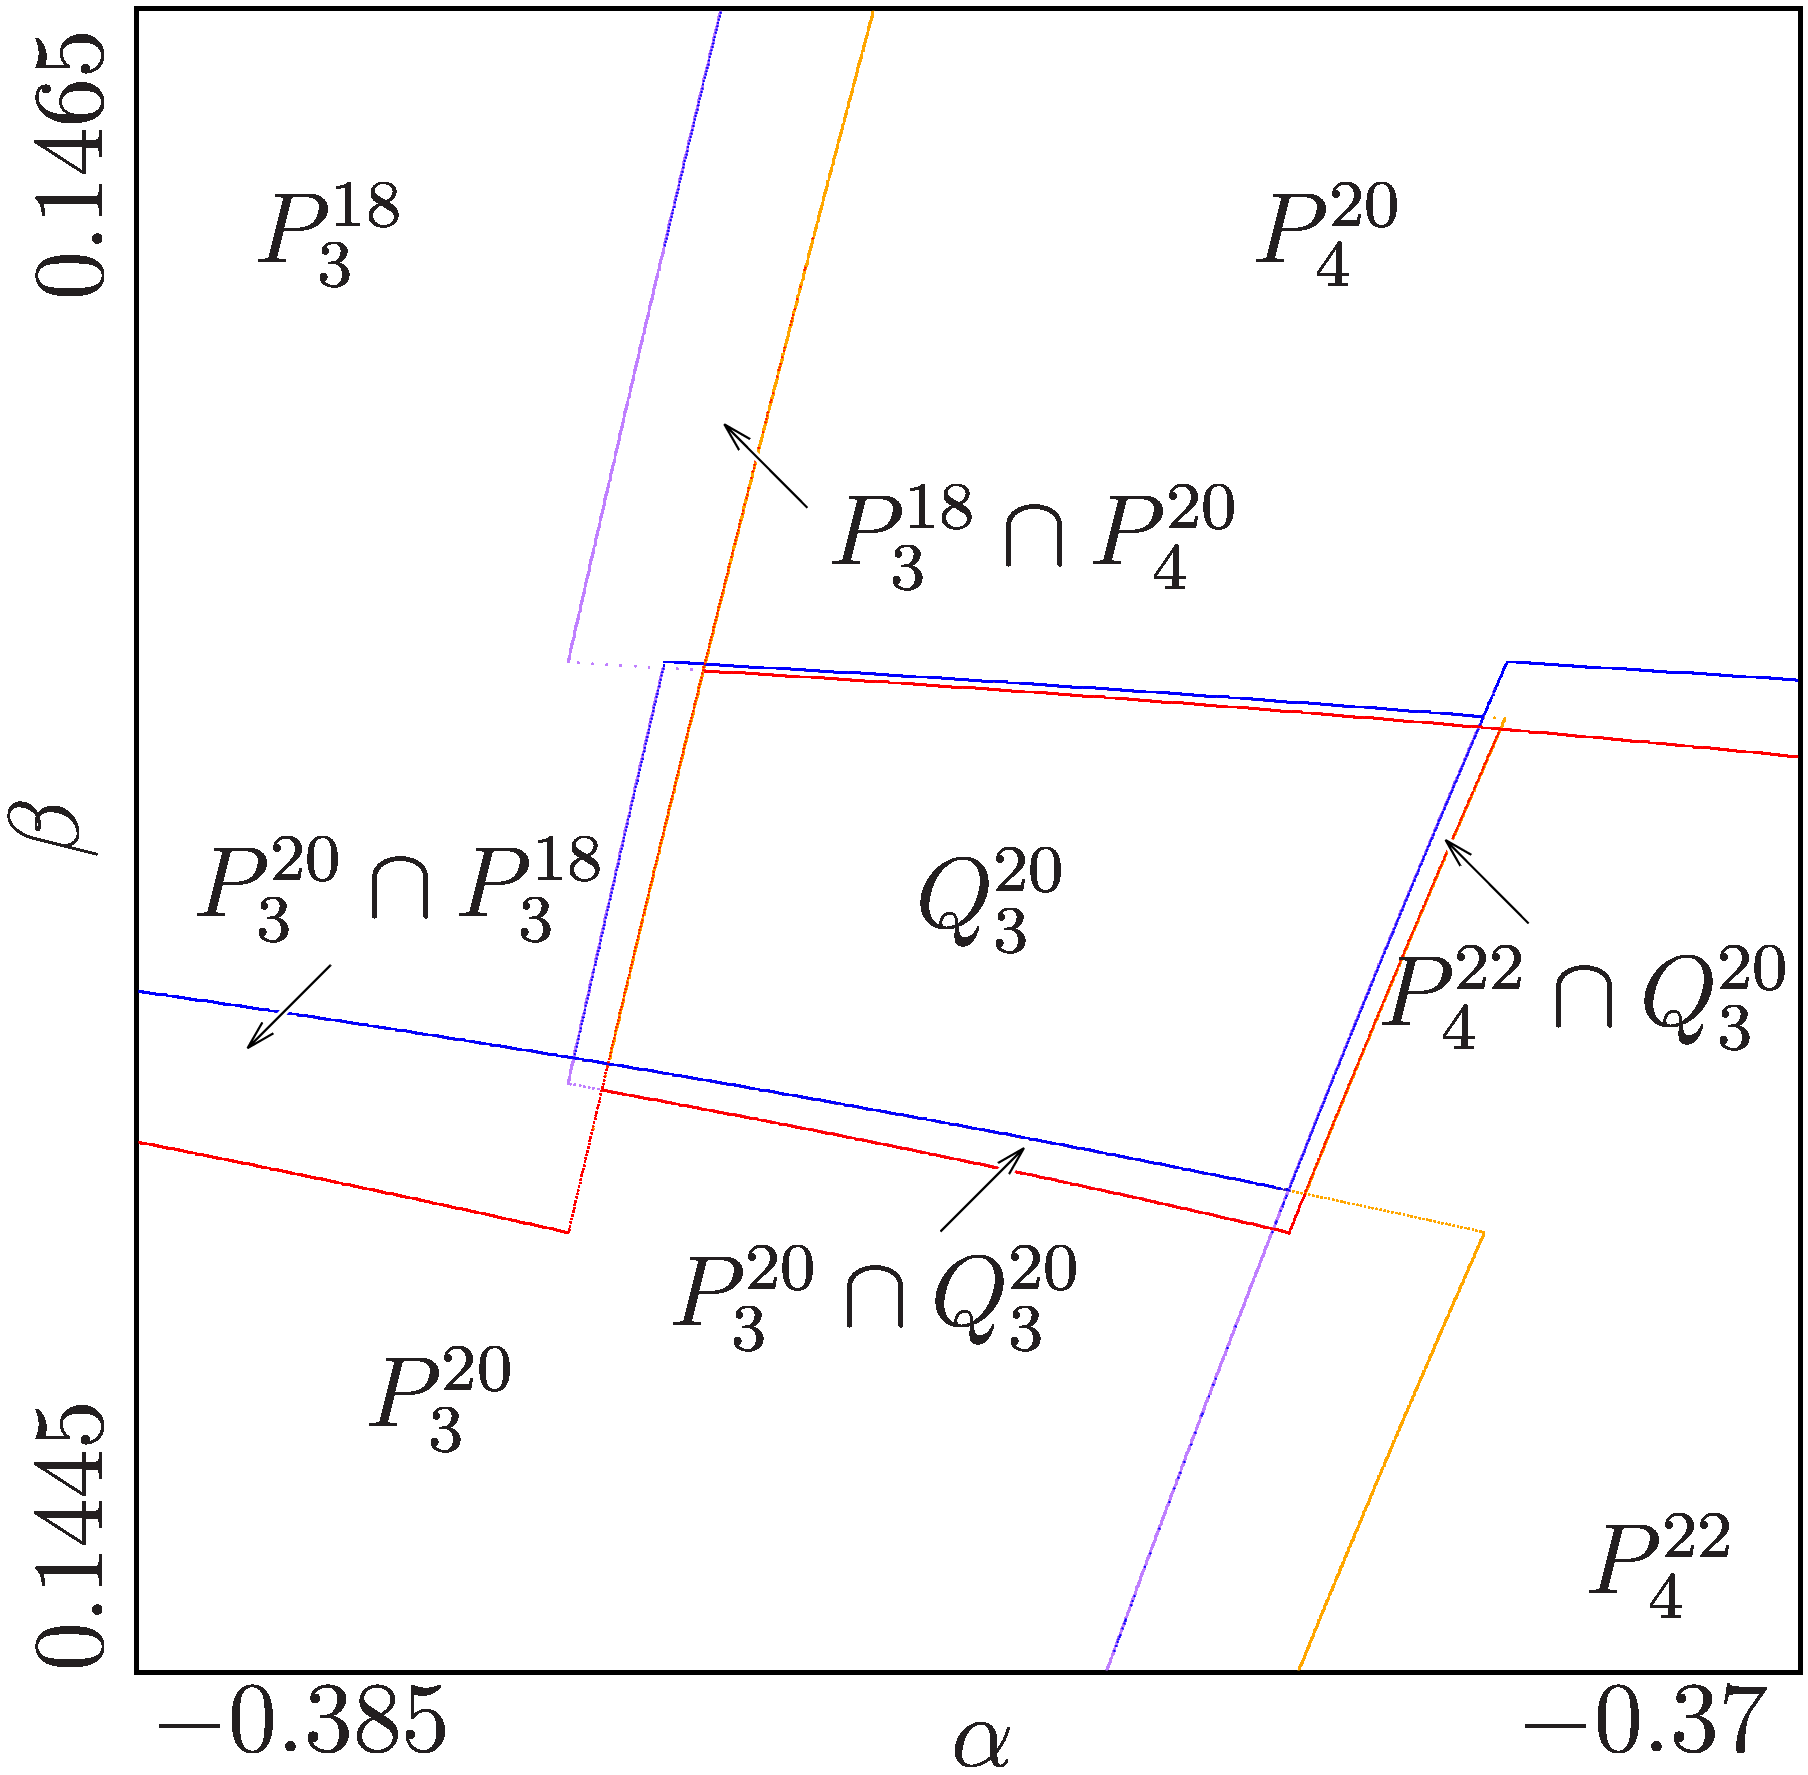
\includegraphics[width=.45 \textwidth]{../Figures/7/7.3a/result.png}
		\label{fig:add.change.regions.1}
	}
	\subfloat[$a_L = 2.8, b_L = -0.1$]{
		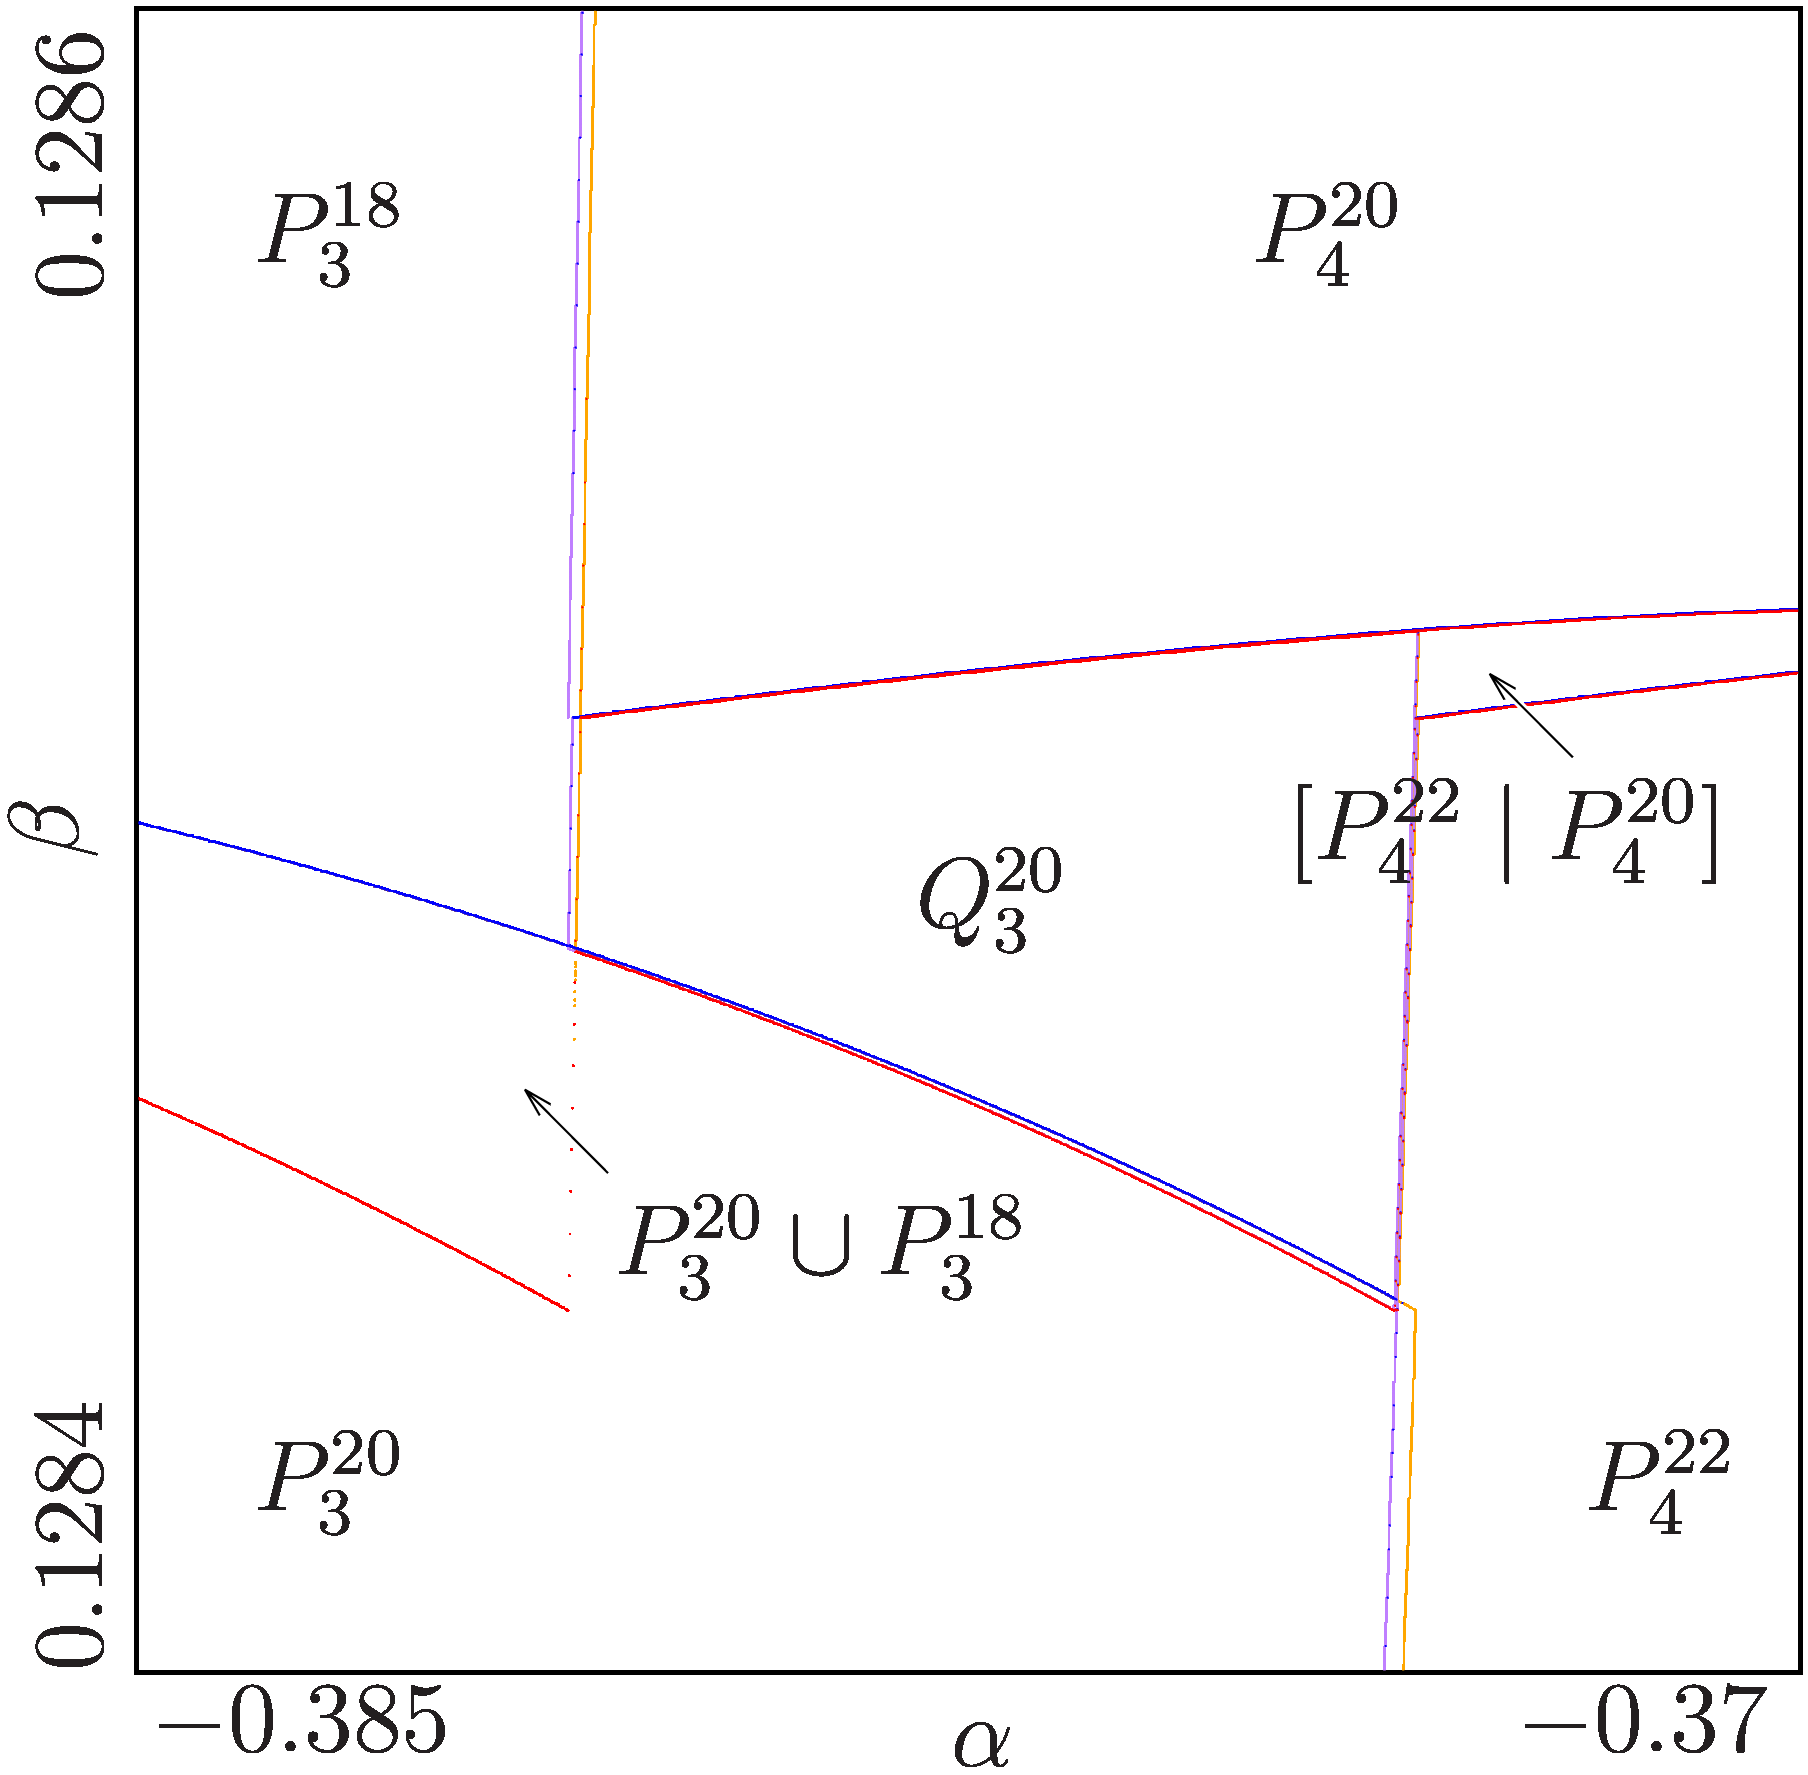
\includegraphics[width=.45 \textwidth]{../Figures/7/7.3b/result.png}
		\label{fig:add.change.regions.2}
	} \\
	\subfloat[$a_L = 2.725, b_L = -0.075$]{
		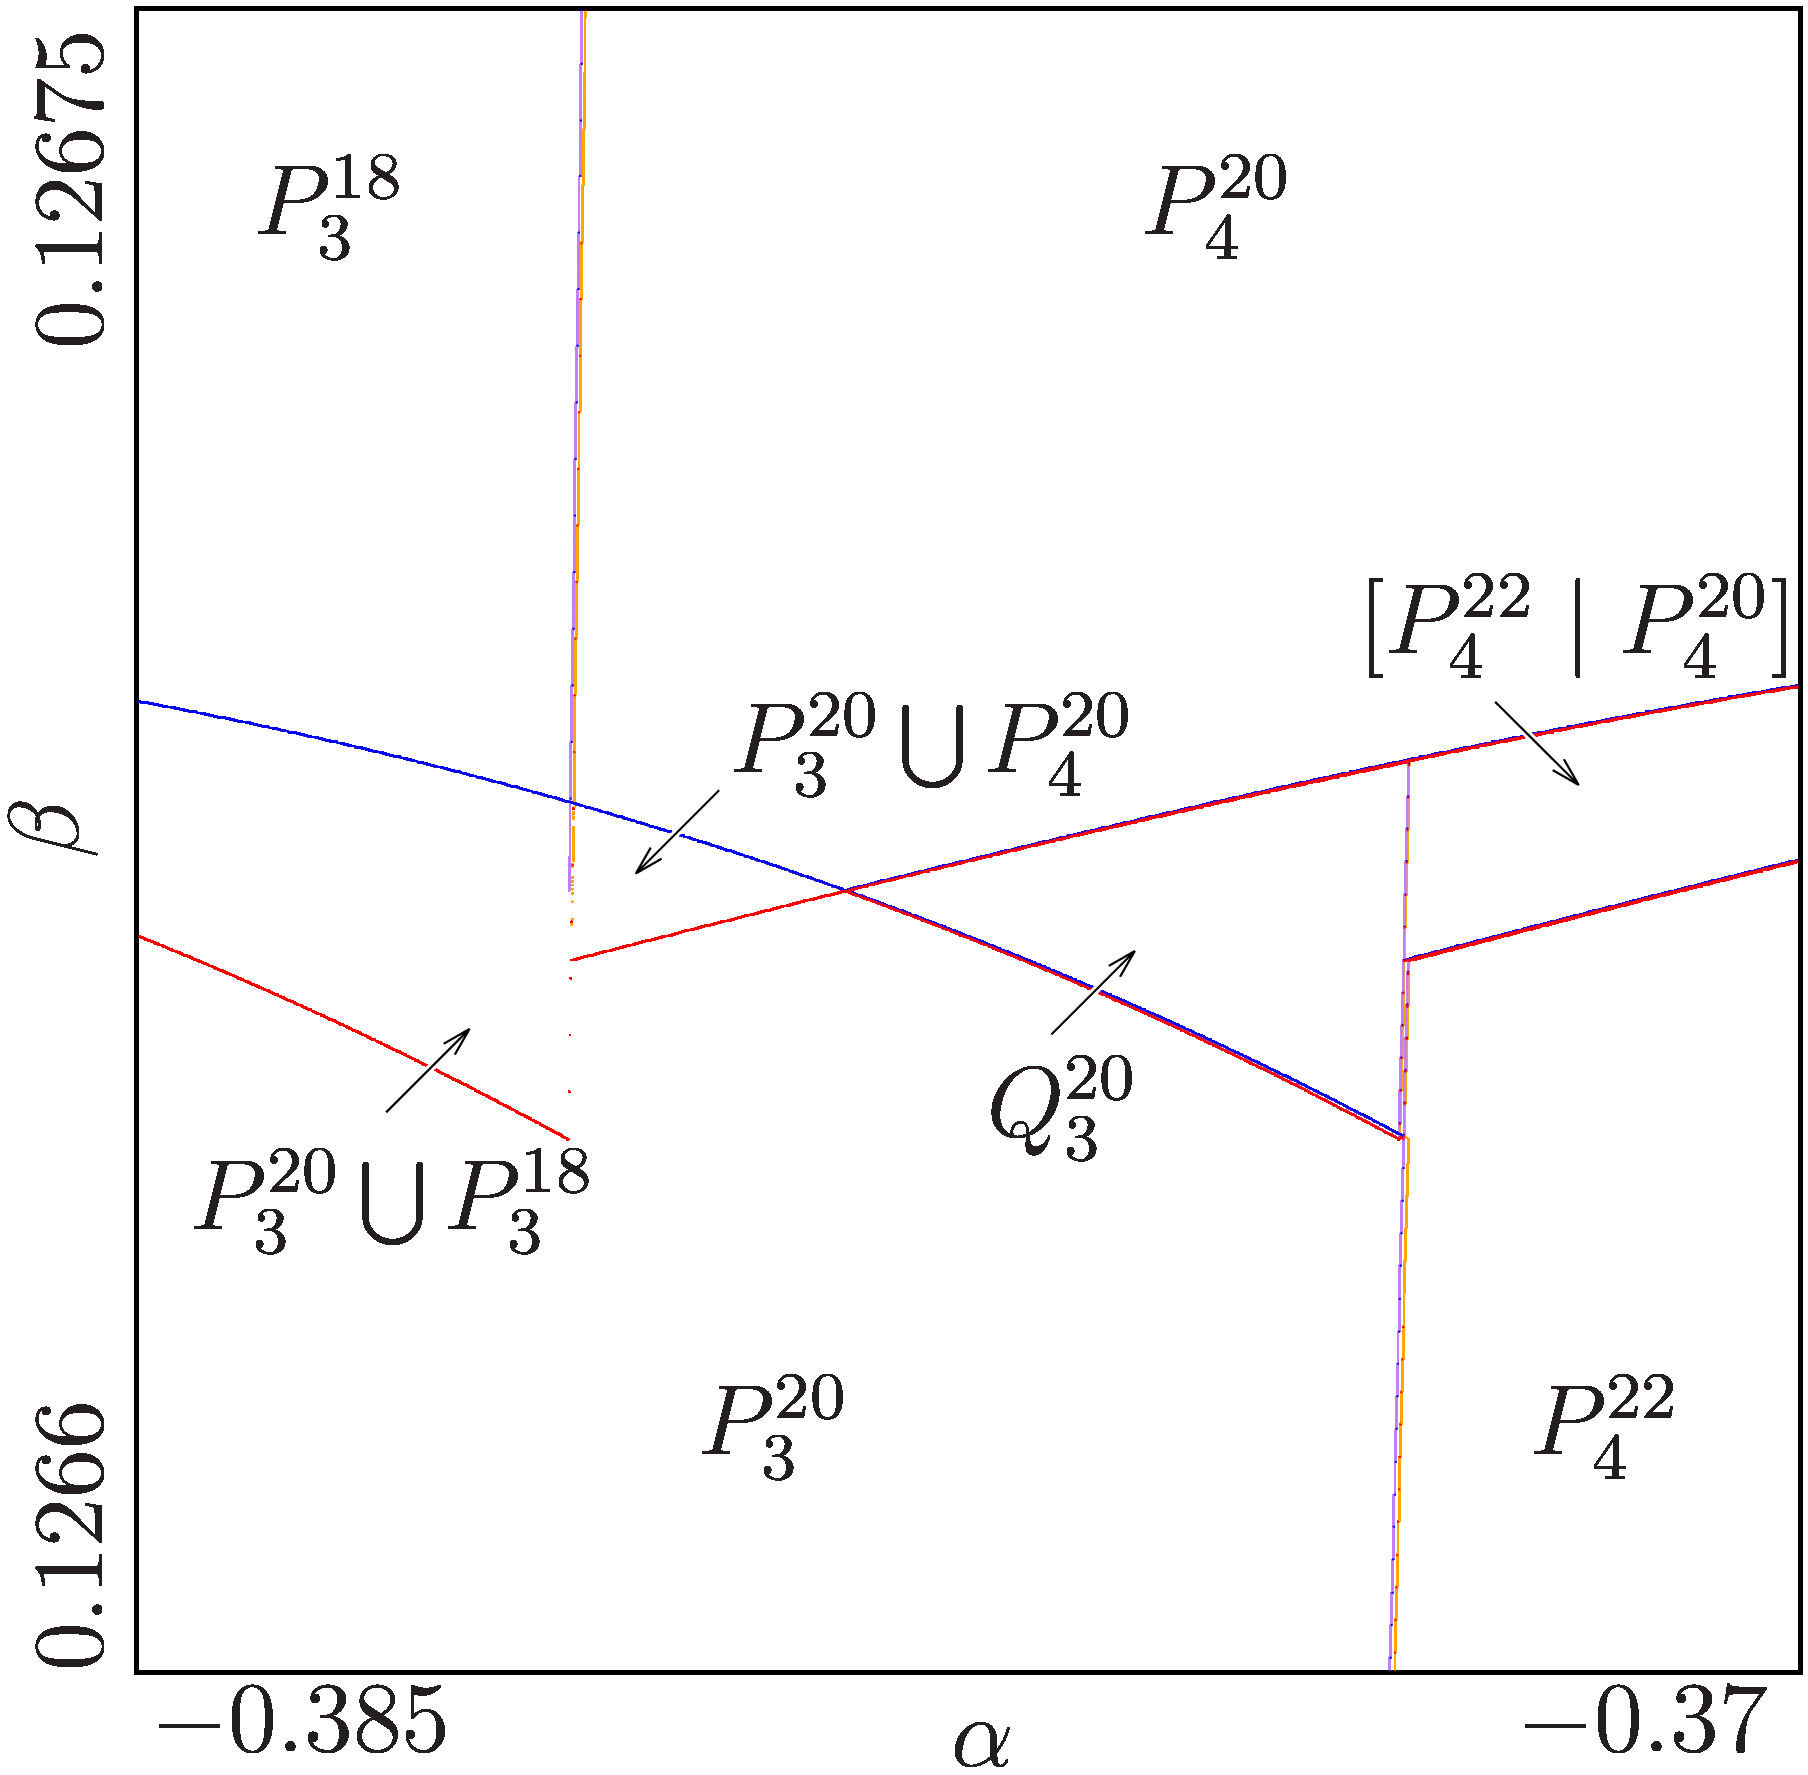
\includegraphics[width=.45 \textwidth]{../Figures/7/7.3c/result.png}
		\label{fig:add.change.regions.3}
	}
	\subfloat[$a_L = 2.5, b_L = 0$]{
		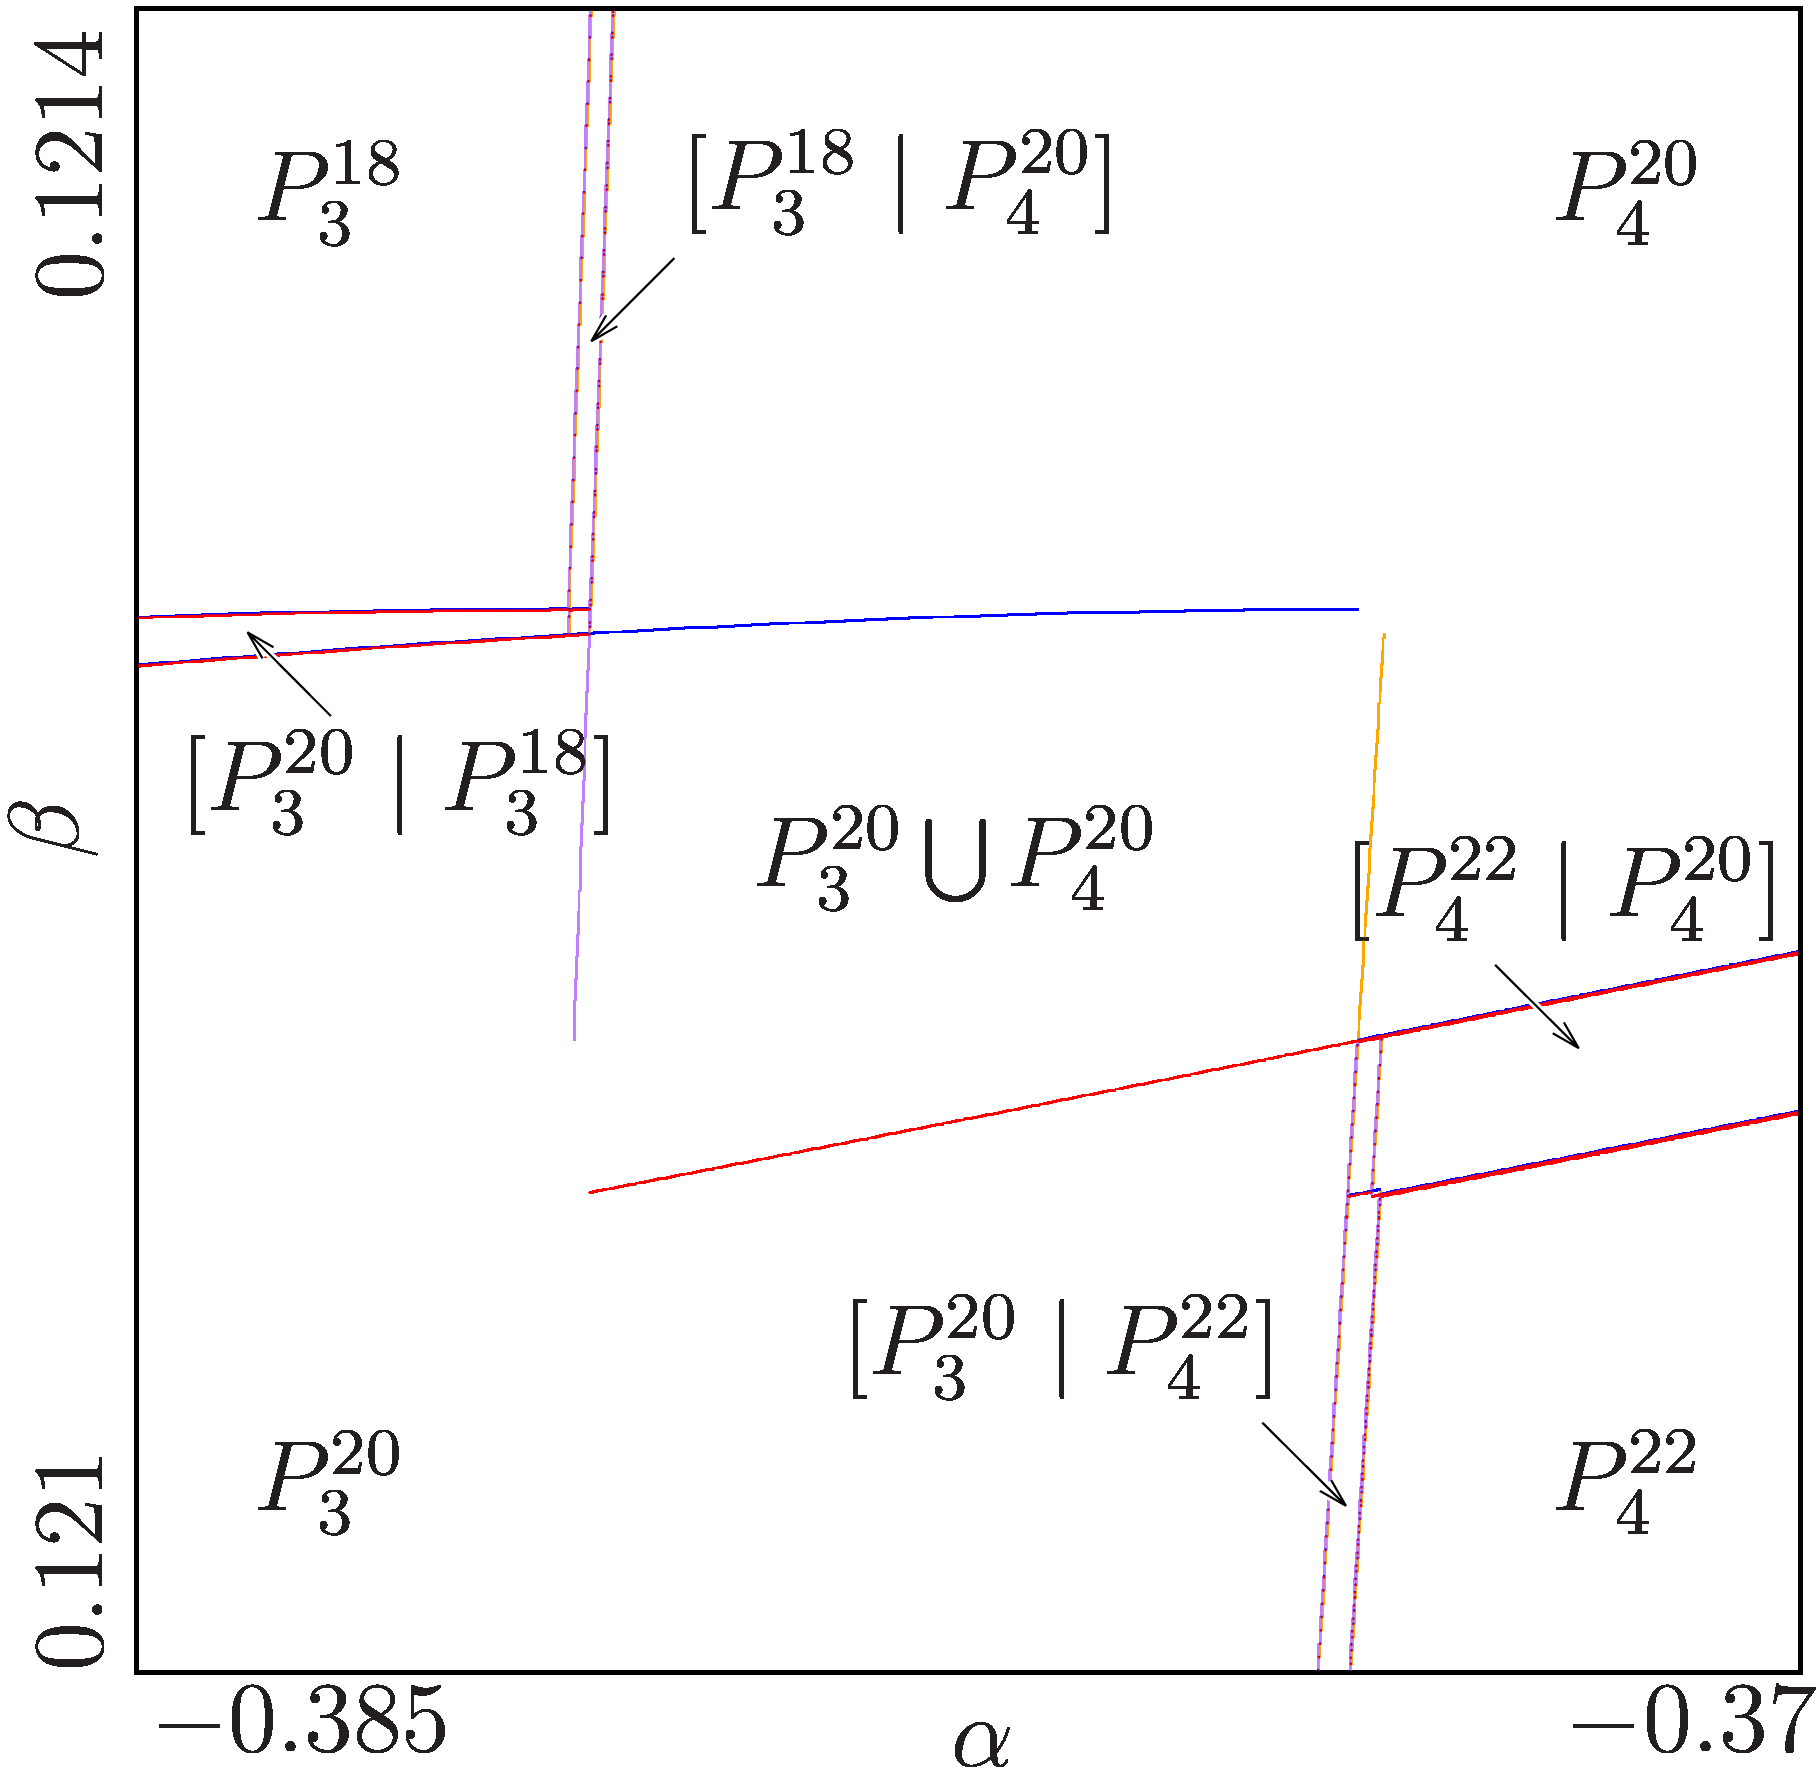
\includegraphics[width=.45 \textwidth]{../Figures/7/7.3d/result.png}
		\label{fig:add.change.regions.4}
	}
	\caption[2D scans of the boundaries of parameter regions associated with different symbolic sequences in the archetypal model showing their evolution when transitioning to increasing branches]{
		2D scans of the boundaries of parameter regions associated with different symbolic sequences in the archetypal model showing their evolution when transitioning to increasing branches.
		The parameter $g_R\left(\frac{1}{2}\right) = \frac{1}{2} + \frac{1}{40}$ is fixed in every diagram.
		The parameters $a_L$ and $b_L$ are fixed, but different in every diagram.
		Their values are on the line given by \Cref{equ:add.change.paramline}.
		The parameter $\alpha = g_R\left(\frac{1}{4}\right)$ is varied in the range $[-0.385, -0.37]$ in every diagram.
		The parameter $\beta = c_L$ is varied in different ranges in every diagram such that the parameter region in the lower left corner is always $P^{20}_3$.
		(a) shows the boundaries for the fixed parameters $a_L = 3.5$ and $b_L = -0.\overline{3}$ with the parameter $\beta$ being varied in the range $[0.1445, 0.1465]$,
		(b) shows the boundaries for the fixed parameters $a_L = 2.8$ and $b_L = -0.1$ with the parameter $\beta$ being varied in the range $[0.1284, 0.1286]$,
		(c) shows the boundaries for the fixed parameters $a_L = 2.75$ and $b_L = -0.075$ with the parameter $\beta$ being varied in the range $[0.1266, 0.12675]$,
		and (d) shows the boundaries for the fixed parameters $a_L = 2.5$ and $b_L = 0$ with the parameter $\beta$ being varied in the range $[0.121, 0.1214]$.
	}
	\label{fig:add.change.regions}
\end{figure}

The disappearance of the ``type B'' parameter regions is examined first in the next section.
The section after that examines the appearance of the \gls{pal} structures between the chains of parameter regions associated with the same period.

\clearpage
\subsection{Disappearance of ``Type B'' Parameter Regions}
\label{sec.change.disb}

For \Cref{fig:add.change.regions.1,fig:add.change.regions.2}, the ``type B'' parameter region $Q^{20}_3$ is complete.
In \Cref{fig:add.change.regions.4}, it is gone completely, instead the two ``type A'' parameter regions $P^{20}_3$ and $P^{20}_4$ now overlap.
\todo{In regions figure 3: labels $P^{20}_2$ wrong, should be $P^{20}_4$}

In between those two stages, we can see how the ``type B'' parameter region $Q^{20}_3$ disappears.
\Cref{fig:add.change.regions.3} shows the ``type A'' parameter regions $P^{20}_3$ and $P^{20}_4$ overlapping.
The point, where their boundaries cross is in the middle of where the ``type B'' parameter region was in \Cref{fig:add.change.regions.2}.
This point is also where the ``type B'' parameter region now ends.

\todo{Labels in figure wrong!}
\todo{In cobweb diagrams: enhance cycles at borders}
\begin{figure}
	\centering
	\subfloat[Regions]{
		\includegraphics[width=.3 \textwidth]{62_MinimalRepr_Adding/2D_Regions_2.675/Manual/result.png}
		\label{fig:add.change.disb.regions}
	}
	\subfloat[Cobweb at point $A$]{
		\includegraphics[width=.3 \textwidth]{62_MinimalRepr_Adding/Cob_2.675_A/Manual/result.png}
		\label{fig:add.change.disb.cob.A}
	}
	\subfloat[Cobweb at point $B$]{
		\includegraphics[width=.3 \textwidth]{62_MinimalRepr_Adding/Cob_2.675_B/Manual/result.png}
		\label{fig:add.change.disb.cob.B}
	}
	\caption{Disappearance of the ``type B'' parameter region}
\end{figure}

\Cref{fig:add.change.disb.regions} shows the same thing as \Cref{fig:add.change.regions.3} again but at parameter value closer to the diappearence of the ``type B'' parameter region.
We can see that the point where the boundaries of the ``type A'' parameter regions cross moved right and the ``type B'' parameter region got smaller.
This point is called a codimension-2 point because at this point, two bifurcations happen at the same time to the same cycle.

We know from \Cref{sec:arch.bif.sum} that the \gls{bcb} at the upper boundary of the ``type A'' parameter region $P^{20}_3$ is $\BCB_{d_1, d_3}^{\underline{\A}^7\B^3\underline{\C}^7\D^3}$.
And the \gls{bcb} at the lower boundary of the ``type A'' parameter region $P^{20}_4$ is $\BCB_{d_1, d_3}^{\A^6\underline{\B}^4\C^6\underline{\D}^4}$.
At the codimension-2 point, both these \glspl{bcb} happen at the same time and both cycles vanish.
We can see in \Cref{fig:add.change.disb.cob.A} that the ``type A'' cycles are very close to the borders $d_1$ and $d_3$, respectively.

We also know that the \glspl{bcb} at the top of the ``type B'' parameter region $Q^{20}_3$ are $\BCB_{d_1}^{\underline{\A}^7\B^3\C^6\D^4}$ and $\BCB_{d_3}^{\A^6\B^4\underline{\C}^7\D^3}$.
And the \glspl{bcb} at the lower boundary are $\BCB_{d_3}^{\A^7\B^3\C^6\underline{\D}^4}$ and $\BCB_{d_1}^{\A^7\underline{\B}^3\C^6\D^4}$.
At the codimension-2 point, both \glspl{bcb} $\BCB_{d_1}^{\underline{\A}^7\B^3\C^6\D^4}$ and $\BCB_{d_3}^{\A^7\B^3\C^6\underline{\D}^4}$ happen to the cycle $\Cycle{\A^7\B^3\C^6\D^4}$ at the same time and it vanishes.
Because of the symmetry, the \glspl{bcb} $\BCB_{d_3}^{\A^6\B^4\underline{\C}^7\D^3}$ and $\BCB_{d_1}^{\A^7\underline{\B}^3\C^6\D^4}$ happen to the cycle $\Cycle{\A^6\B^4\C^7\D^3}$ at the same time and it vanishes also.

This codimension-2 point moves right with higher values for $b_L$ along our line.
As soon as the codimension-2 point crosses the right boundary of the ``type B'' parameter region, the ``type B'' parameter region ceases to exist.
Instead, now the two ``type A'' parameter regions overlap without the codimension-2 point.
This new overlapping regions is bounded by simple ``type A'' boundary \glspl{bcb} as they are discussed in \Cref{sec:arch.bif.sum}.

\todo{Confirm bcbs with cobweb diagrams}

\todo{Order of left most cycle and other cycle => type B or type A. idk}

\subsection{Appearance of Period-adding structures}

In this section we will explore the appearance of the period-adding structures in between the chains of the same period.
This happens at the horizontal boundaries between ``type A'' parameter regions of different chains, as well as at the vertical boundaries.
We will first take care of the horizontal period-adding structures and then move on to the vertical period-adding structures.

\subsubsection{Horizontal Period-adding Structures}

In \Cref{fig:add.change.regions.1}, the ``type A'' parameter regions $P^{20}_3$ and $P^{18}_3$, as well as $P_{22}_4$ and $P^{20}_4$ overlap.
This changes in \Cref{fig:add.change.regions.2}.
Here only the ``type A'' parameter regions $P^{20}_3$ and $P^{18}_3$ overlap, the parameter regions $P_{22}_4$ and $P^{20}_4$ stopped overlapping.
Instead, in the space between the two ``type A'' parameter region there are now two asymmetric coexisting twin cycles $\Cycle{\A^8\B^3\C^8\D^2}$ and $\Cycle{\A^8\B^2\C^8\D^3}$.
Those cycles are \textbf{not} ``type B'' cycles, because they only differ in the number of points on the branches $f_\B$ and $f_\D$.
Instead, we will call them hybrid cycles and ``type B'' cycles are a special case of hybrid cycles.
The notation $\left[P^{22}_4 \mid P^{20}_4\right]$ used in the diagrams was introduced in \Cref{sec:add.change} and is formally defined later in \Cref{sec:add.add.halved}.
Later in \Cref{fig:add.change.regions.4}, the ``type A'' parameter regions $P^{20}_3$ and $P^{18}_3$ also stop overlapping.
In between, there are also hybrid cycles, $\Cycle{\A^7\B^3\C^6\D^3}$ and $\Cycle{\A^6\B^3\C^7\D^3}$.
This parameter region is therefore labeled $\left[P^{20}_3 \mid P^{18}_3\right]$.

In between \Cref{fig:add.change.regions.2,fig:add.change.regions.3}, the ``type A'' parameter regions $P_{22}_4$ and $P^{20}_4$ don't stop overlapping completely.
Instead, they only stop overlapping on the left side of their shared boundaries and the rest is not pictured in these diagrams.
\Cref{fig:add.change.appa.hor.regions} shows better what happens to this overlapping region between \Cref{fig:add.change.regions.1,fig:add.change.regions.4}.
We also have a codimension-2 point that moves right as was the case in \Cref{sec:add.change.disb}.

\todo{Regions: labels wrong}
\todo{Cobwebs: enhance borders, replace (c), wrong pic}
\begin{figure}
	\centering
	\subfloat[Regions]{
		\includegraphics[width=.3 \textwidth]{62_MinimalRepr_Adding/2D_Regions_2.8_add_hor/Manual/result.png}
		\label{fig:add.change.appa.hor.regions}
	}
	\subfloat[At point $A$]{
		\includegraphics[width=.3 \textwidth]{62_MinimalRepr_Adding/Cob_2.8_add_hor_A/Manual/result.png}
		\label{fig:add.change.appa.hor.cob.A}
	}
	\subfloat[At point $B$]{
		\includegraphics[width=.3 \textwidth]{62_MinimalRepr_Adding/Cob_2.8_add_hor_A/Manual/result.png}
		\label{fig:add.change.appa.hor.cob.B}
	}
	\caption{Appearance of the horizontal period-adding cascade}
\end{figure}

We know from \Cref{sec:arch.bif.sum} that the \gls{bcb} at the upper boundary of the ``type A'' parameter region $P^{22}_4$ is $\BCB_{d_1, d_3}^{\underline{\A}^7\B^4\underline{\C}^7\D^4}$.
And the \gls{bcb} at the lower boundary of the ``type A'' parameter region $P^{20}_4$ is $\BCB_{d_1, d_3}^{\A^6\underline{\B}^4\C^6\underline{\D}^4}$.
Both these \glspl{bcb} are at the upper and lower boundaries of the overlapping region $P^{22}_4 \Cup P^{20}_4$.
At the codimension-2 point, both these \glspl{bcb} happen at the same time and both cycles vanish.
We can see in \Cref{fig:add.change.appa.hor.cob.A} that the ``type A'' cycles are very close to the borders $d_1$ and $d_3$, respectively.

This codimension-2 point moves right with higher values for $b_L$ along our line.
As soon as the codimension-2 point crosses the right boundary of either the ``type A'' parameter region $P^{22}_4$ or $P^{20}_4$, the overlapping parameter region $P^{22}_4 \Cup P^{20}_4$ ceases to exist.
Instead, there is space between the two ``type A'' parameter regions where the are now two hybrid cycles and period-adding between the hybrid cycles and either ``type A'' parameter region.

\todo{Labels for bifurcations missing underline}
\begin{figure}
	\centering
	\includegraphics[width=.7 \textwidth]{62_MinimalRepr_Adding/1D_Bif_2.8_add_hor_AU/Manual/result.png}
	\caption{Bifurcation diagram at the upper boundary of $\left[P^{22}_4 \mid P^{20}_4\right]$}
	\label{fig:add.change.appa.hor.bif}
\end{figure}

We assume that the \glspl{bcb} bounding the parameter regions with hybrid cycles follow the same rules as the \glspl{bcb} bounding the ``type B'' parameter regions.
\Cref{fig:add.change.appa.hor.bif} confirms this for the upper boundary.
So it is bounded at the top by the \glspl{bcb} $\BCB_{d_1}^{\underline{\A}^7\B^4\C^6\D^4}$ and $\BCB_{d_3}^{\A^6\B^4\underline{\C}^7\D^4}$.
And bounded at the bottom by the \glspl{bcb} $\BCB_{d_3}^{\A^7\B^4\C^6\underline{\D}^4}$ and $\BCB_{d_1}^{\underline{\A}^6\B^4\C^7\D^4}$.
At the codimension-2 point, both \glspl{bcb} $\BCB_{d_1}^{\underline{\A}^7\B^4\C^6\D^4}$ and $\BCB_{d_3}^{\A^7\B^4\C^6\underline{\D}^4}$ happen to the cycle $\Cycle{\A^7\B^4\C^6\D^4}$ at the same time and it vanishes.
Because of the symmetry, the \glspl{bcb} $\BCB_{d_3}^{\A^6\B^4\underline{\C}^7\D^4}$ and $\BCB_{d_1}^{\A^6\underline{\B}^4\C^7\D^4}$ happen to the cycle $\Cycle{\A^6\B^4\C^7\D^4}$ at the same time and it vanishes also.

\todo{also confirmed by cobweb with enhanced cycles at borders}

\todo{Parallels to disappearing type B}

\todo{old:}

In \Cref{sec:minrep.adding.disapp.typeB}, we noted that the asymmetry of the ``type B'' cycles is caused by the negative slope of the function at the left border of branches $f_\A$ and $f_\C$.
Since this maps the cycle that starts further left to the right side of the other cycle.
\todo{
	explain better: diff number of points on branches B and D each (type B) therefore reordering necessary for asymm.
	type b also: split at $d_1, d_3$ as well as $d_2$ and $d_0$, here only $d_1, d_3$ (two boundaries).
	here same number of points so there must be no reordering for asymm
}
This is not the case for the cycles at this point, both cycles start at a point on the branch $f_\A$ with a positive slope and therefore keep the same order.
\todo{positive slope important for period adding!}

\subsubsection{Vertical}

\todo{Regions: labels wrong}
\todo{Cobwebs: replace (c) and enhance cycles at borders}
\begin{figure}
	\centering
	\subfloat[Regions scan before period-adding\\at $a_L = 2.8, b_L = -0.1$]{
		\includegraphics[width=.4 \textwidth]{62_MinimalRepr_Adding/2D_Regions_2.8_add_vert/Manual/result.png}
		\label{fig:minrep.add.app.vert.reg.before}
	}
	\subfloat[Regions with period-adding\\at $a_L = 2.65, b_L = -0.05$]{
		\includegraphics[width=.4 \textwidth]{62_MinimalRepr_Adding/2D_Regions_2.65_add_vert/Manual/result.png}
		\label{fig:minrep.add.app.vert.reg.with}
	} \\
	\subfloat[At point $A$]{
		\includegraphics[width=.4 \textwidth]{62_MinimalRepr_Adding/Cob_2.8_add_vert_A/Manual/result.png}
		\label{fig:minrep.add.app.vert.cob.A}
	}
	\subfloat[At point $B$]{
		\includegraphics[width=.4 \textwidth]{62_MinimalRepr_Adding/Cob_2.65_add_vert_B/Manual/result.png}
		\label{fig:minrep.add.app.vert.cob.B}
	}
	\caption{Appearance of the vertical period-adding cascade}
	\label{fig:minrep.add.app.vert}
\end{figure}

For the vertical period-adding cascade, it is similar.
This time one parameter region scan is not enough because the boundaries of $P_{10}^3$ and $P_{11}^4$ are parallel and therefor $P_{10}^3 \bigcup P_{11}^4$ and $P_{10}^3 \oplus P_{11}^4$ can't exist at the same parameter values of $a_L$ and $b_L$.
\Cref{fig:minrep.add.app.vert.reg.before} shows the situation before the vertical period-adding cascade appears.
Here we can see the overlap of the two ``type A'' parameter regions $P_{10}^3$ and $P_{11}^4$.
When changing the parameters a little, we get \Cref{fig:minrep.add.app.vert.reg.with}.
Here the two ``type A'' parameter regions drifted apart and in between them, there is the parameter region $P_{10}^3 \oplus P_{11}^4$.
The notation hints at the period-adding-like nature of this parameter region.

As with the horizontal period-adding cascade, the cycles here are asymmetrical, but not of ``type B''.
\Cref{fig:minrep.add.app.vert.cob.B} shows the cycles at point $B$, in the period adding cascade, $\Cycle{\A^7\B^3\C^7\D^4}$ and its twin $\Cycle{\A^7\B^4\C^7\D^3}$.
Again, interpreted in the context of the halved model, these cycles are both $\Cycle{\L^7\R^3\L^7\R^4} \equiv \Cycle{\L^7\R^4\L^7\R^3}$.
But this time, the splits are not at borders $d_1$ and $d_3$, but at $d_0$ and $d_2$.
\todo{odd number of splits => no neg slope needed for asymmetry. odd number => needed (reorders cycles)}

\begin{figure}
	\centering
	\includegraphics[width=.7 \textwidth]{62_MinimalRepr_Adding/1D_Bif_2.65_add_vert_BR/Manual/result.png}
	\caption{Bifurcation diagram of the right boundary of $P_{10}^3 \oplus P_{11}^4$}
	\label{fig:minrep.add.app.vert.bif.BR}
\end{figure}

Here, the period-adding region opened up enough to see the next stage, colored in purple.
As with the previous bifurcations of the first stage of the horizontal period-adding cascade, the bifurcations are similar to the bifurcations of ``type B'' cycles in \Cref{sec:minrep.bif.R}.
They involve the borders $d_0$ and $d_2$.
\todo{etc}

\subsection{Summary of the Changes to the Bifurcation Structure}

This section summarizes all the changes that happen to the \gls{pi} structure of the archetypal model when the parameters are changed in such a way that \gls{pal} structures emerge.
Furthermore, it provides an explanation for why the \gls{pi} structure of the archetypal model is impossible with only increasing branches.

\subsubsection{Schematics and Summary of the Changes}

\begin{figure}
	\centering
	\subfloat[]{
		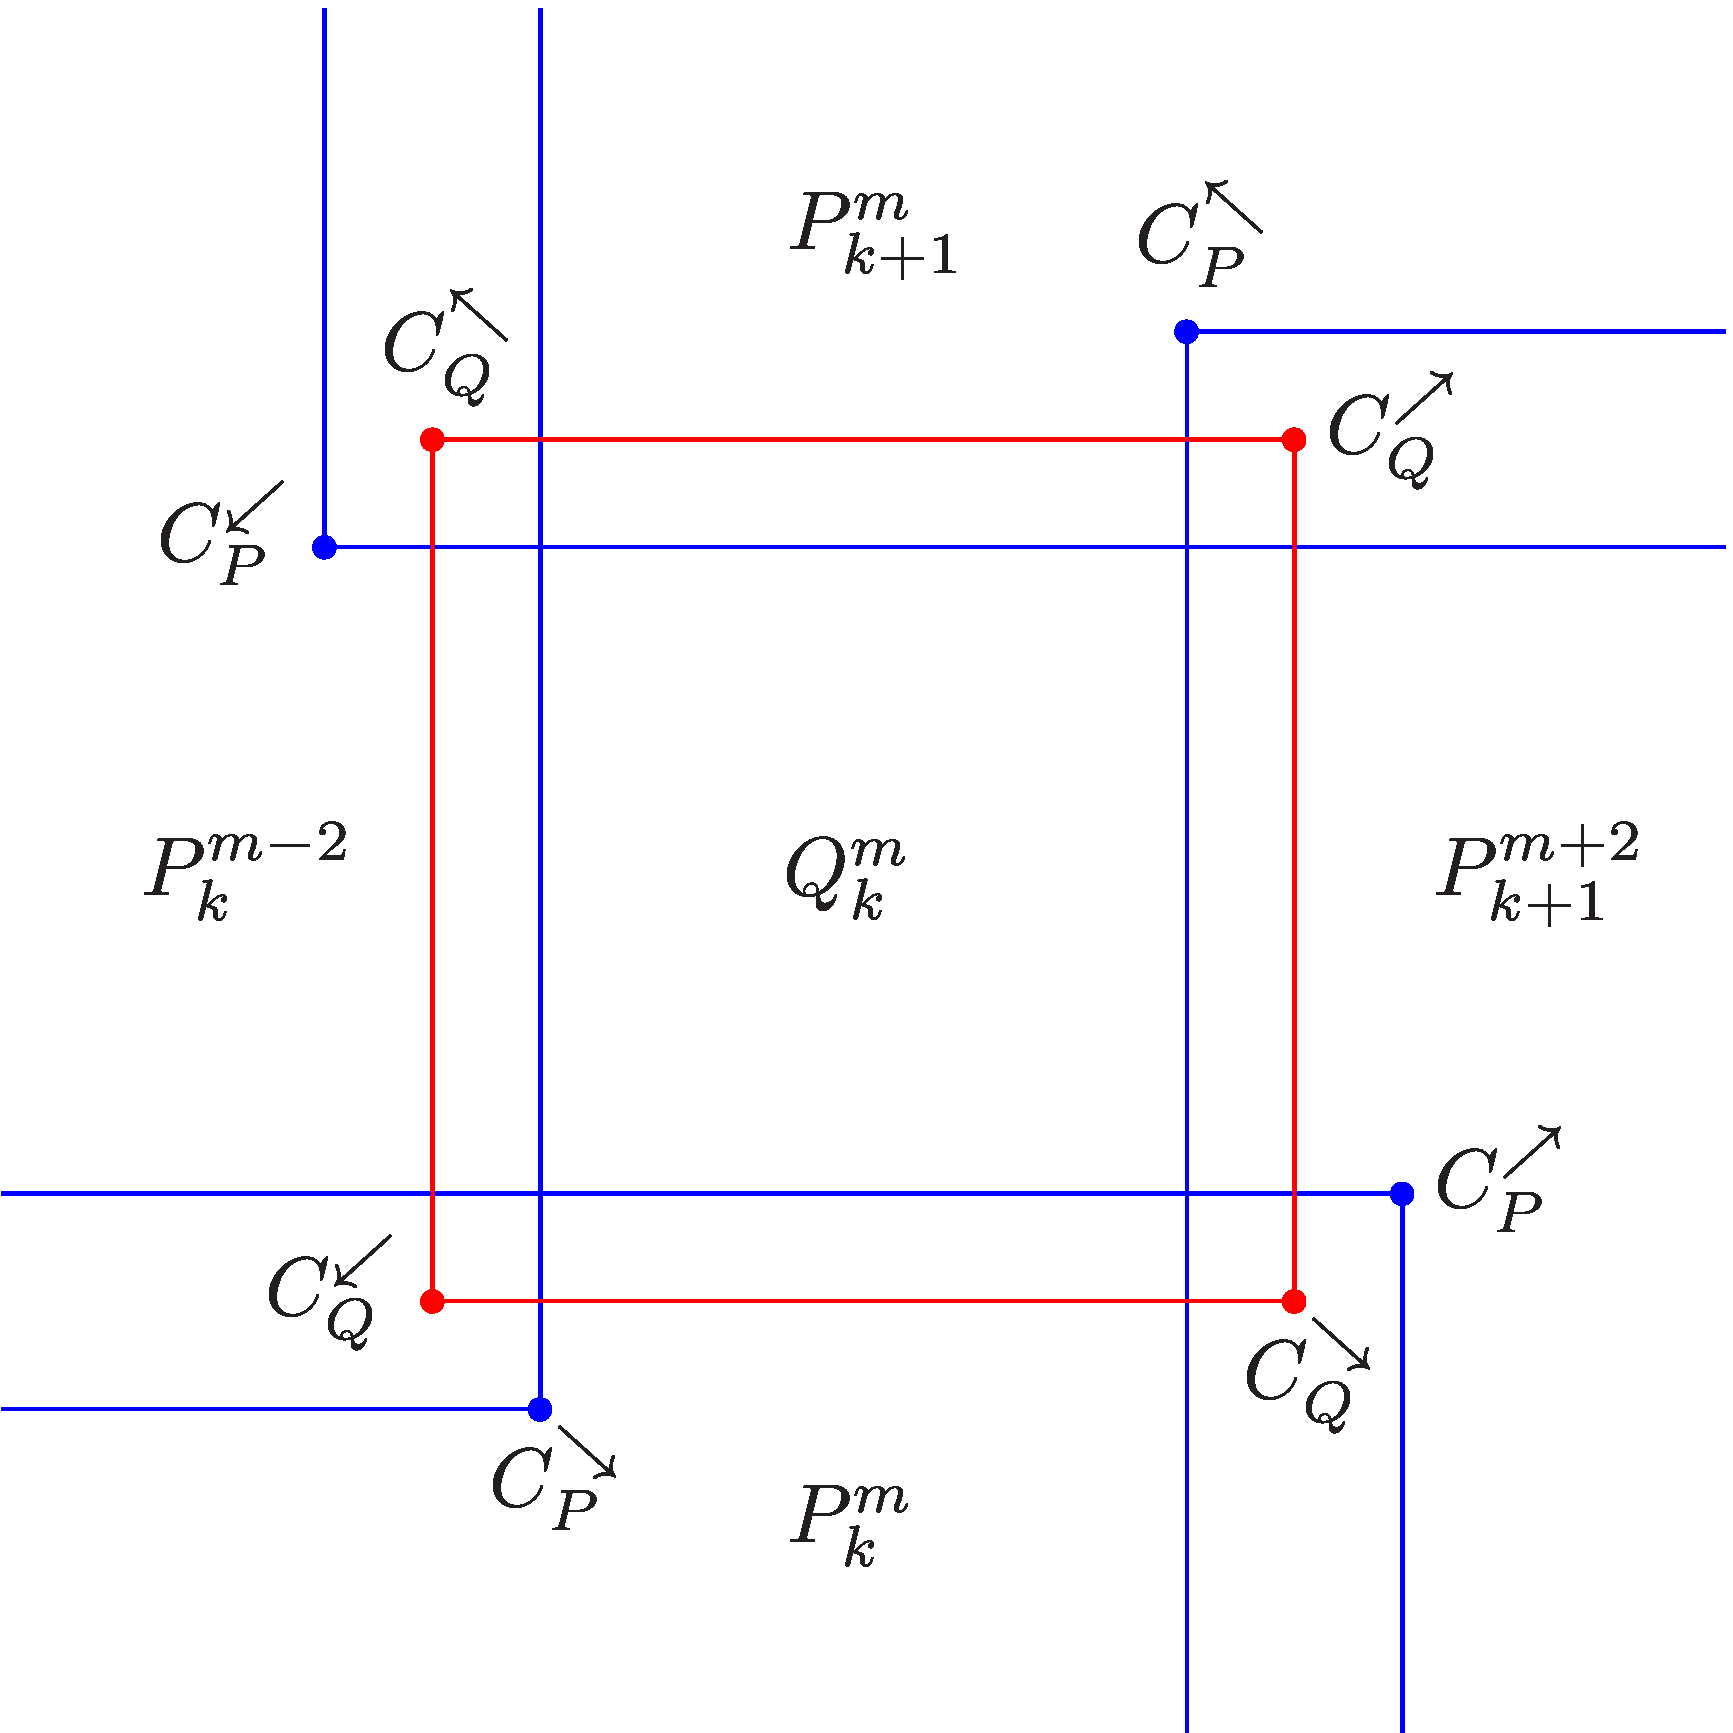
\includegraphics[width=.4 \textwidth]{../Figures/7/7.9a/result.png}
		\label{fig:add.change.schema.a}
	}
	\subfloat[]{
		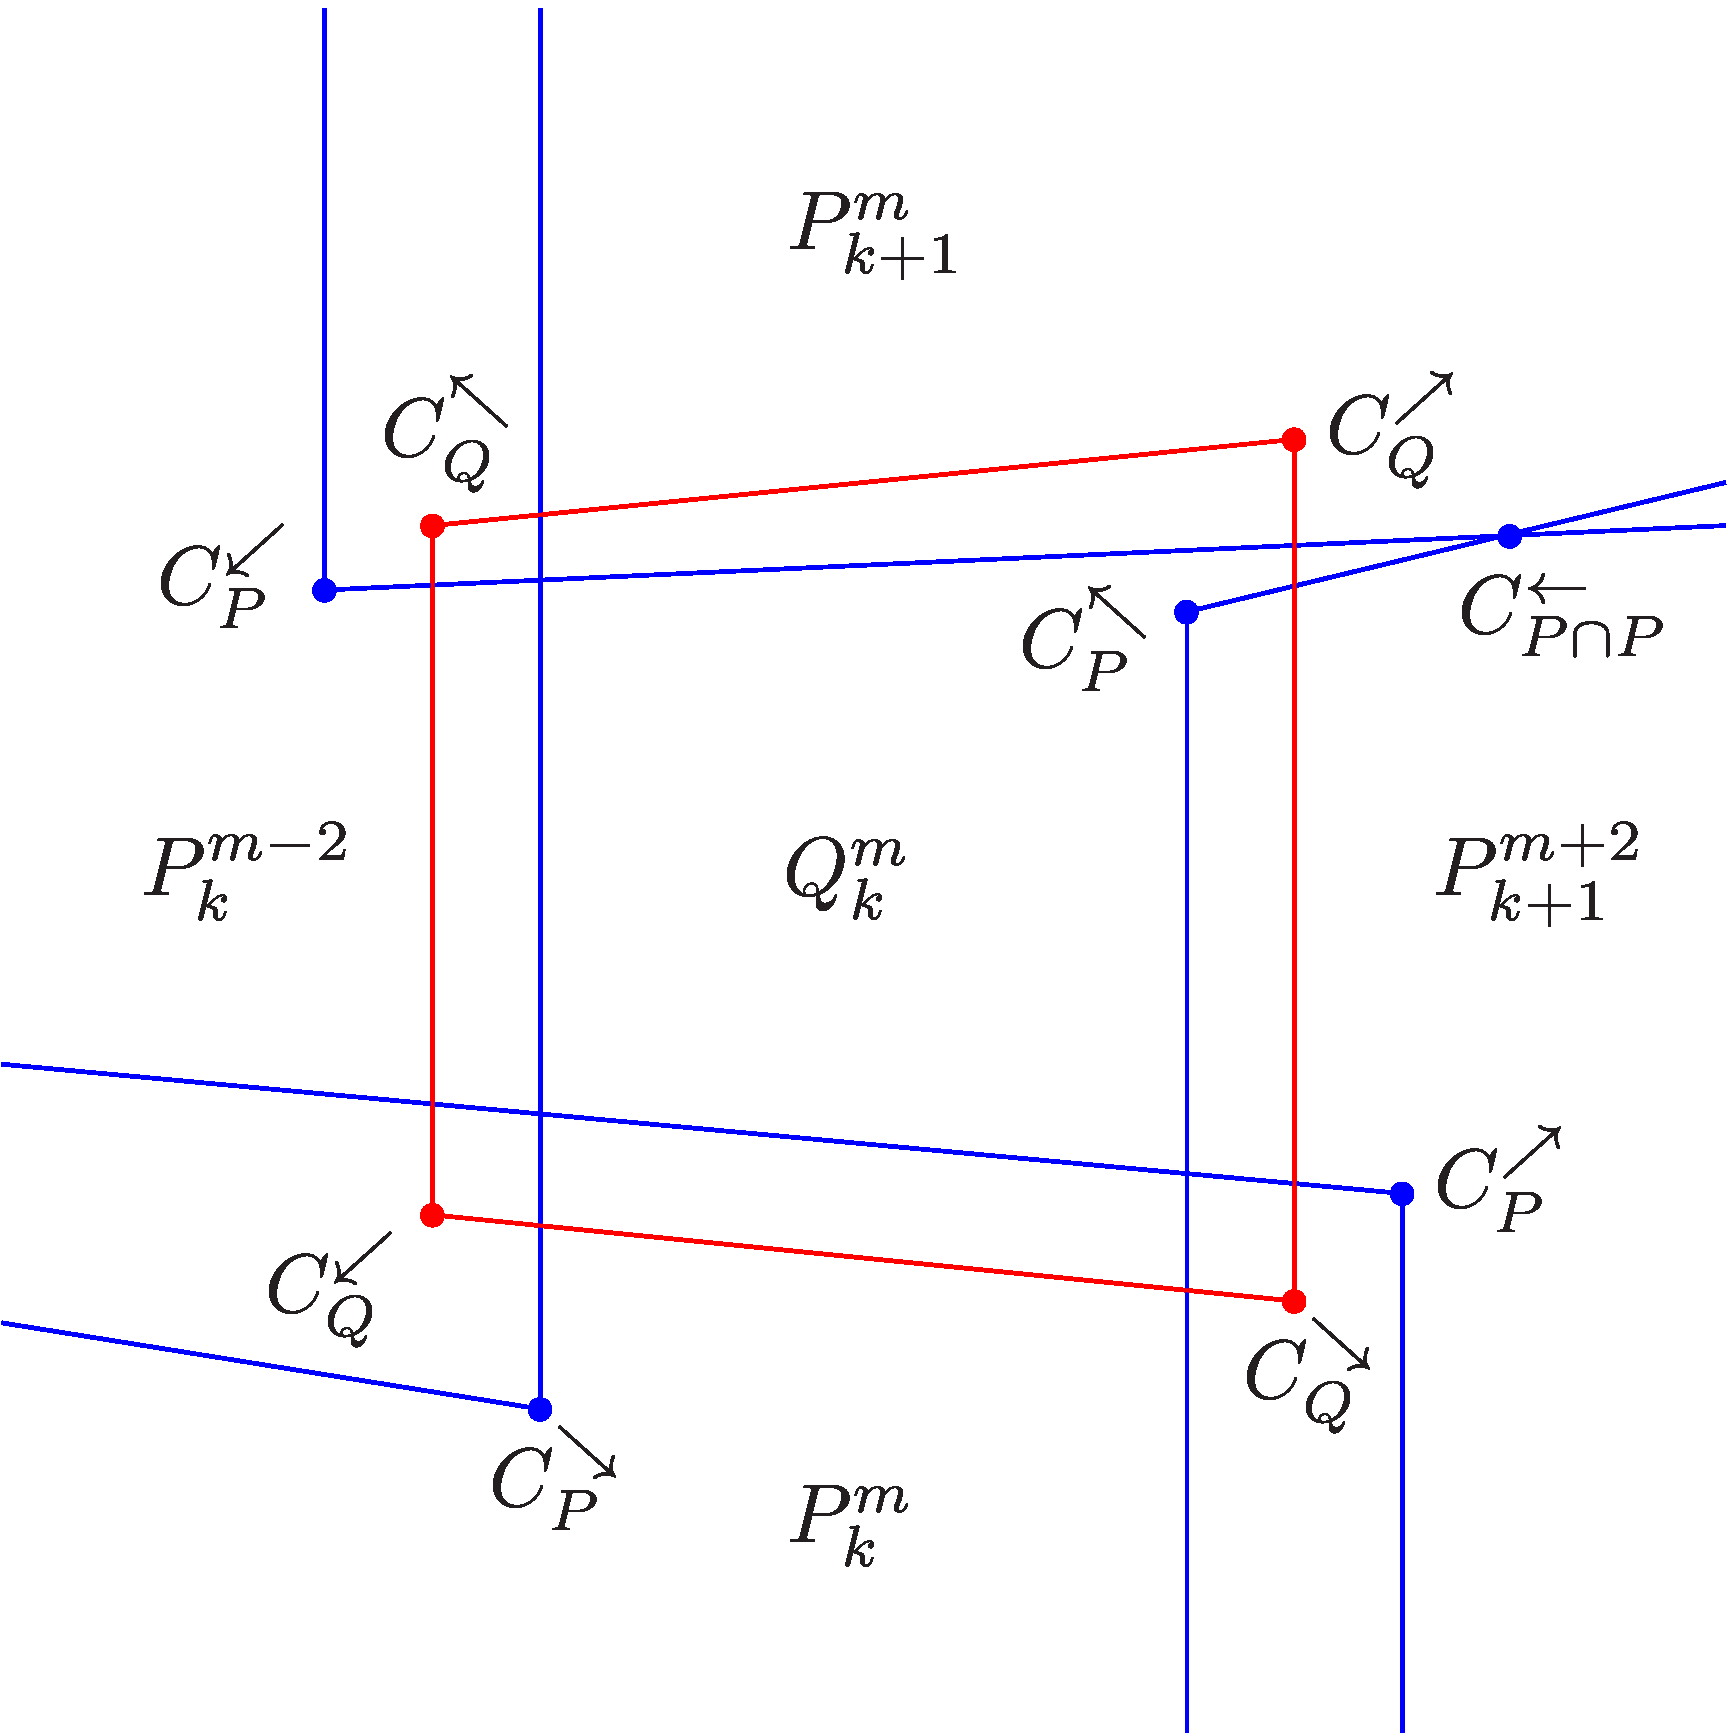
\includegraphics[width=.4 \textwidth]{../Figures/7/7.9b/result.png}
		\label{fig:add.change.schema.b}
	} \\
	\subfloat[]{
		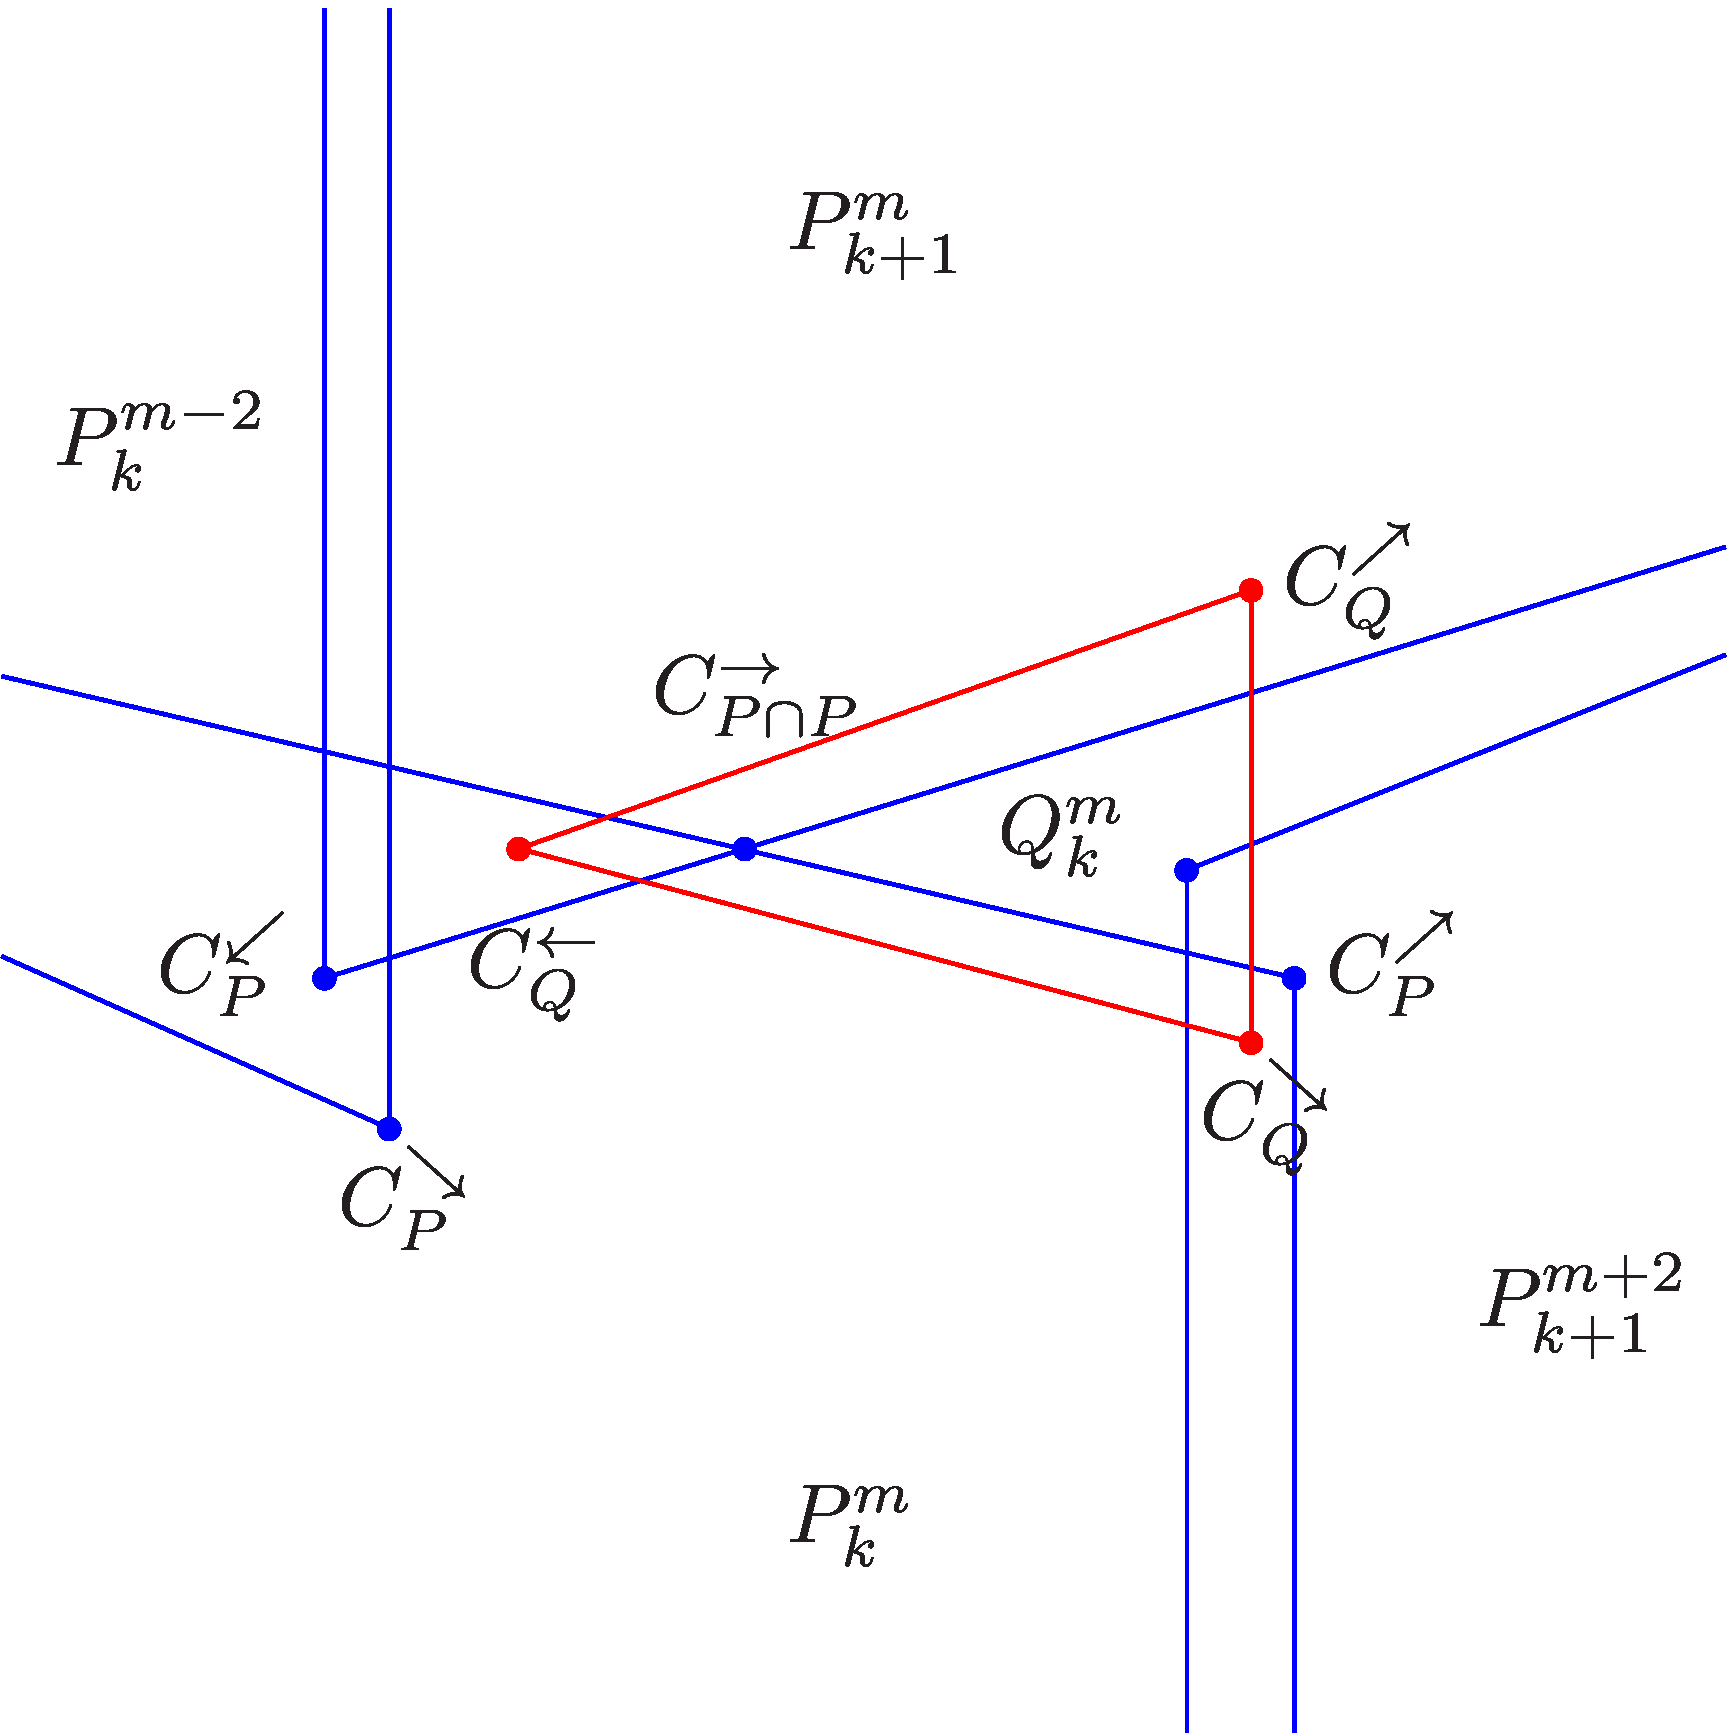
\includegraphics[width=.4 \textwidth]{../Figures/7/7.9c/result.png}
		\label{fig:add.change.schema.c}
	}
	\subfloat[]{
		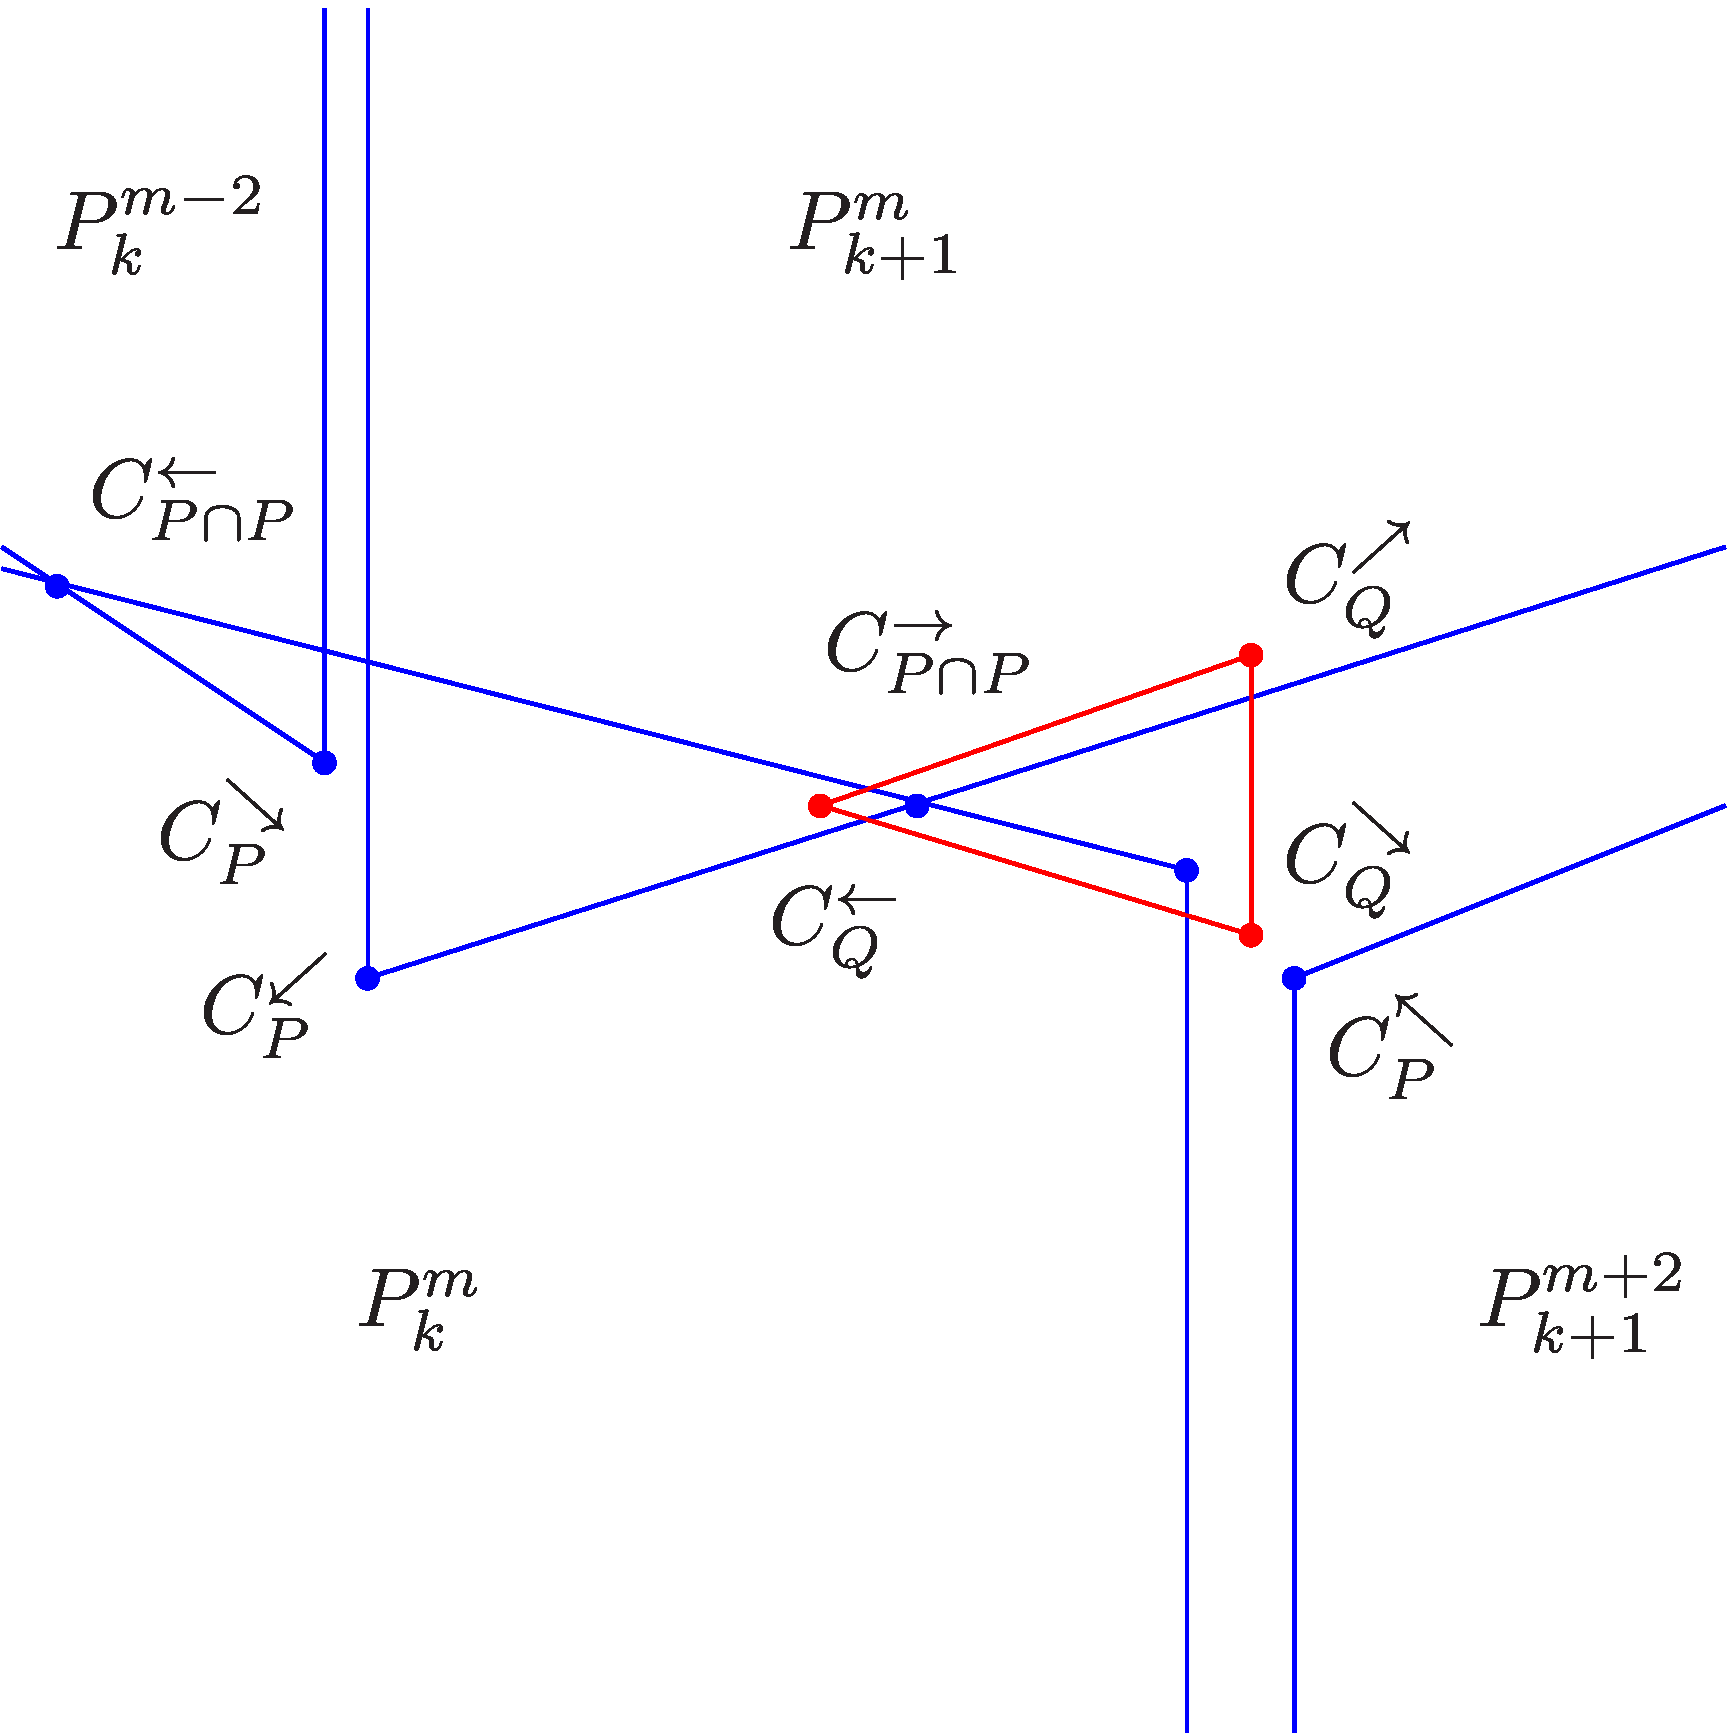
\includegraphics[width=.4 \textwidth]{../Figures/7/7.9d/result.png}
		\label{fig:add.change.schema.d}
	} \\
	\subfloat[]{
		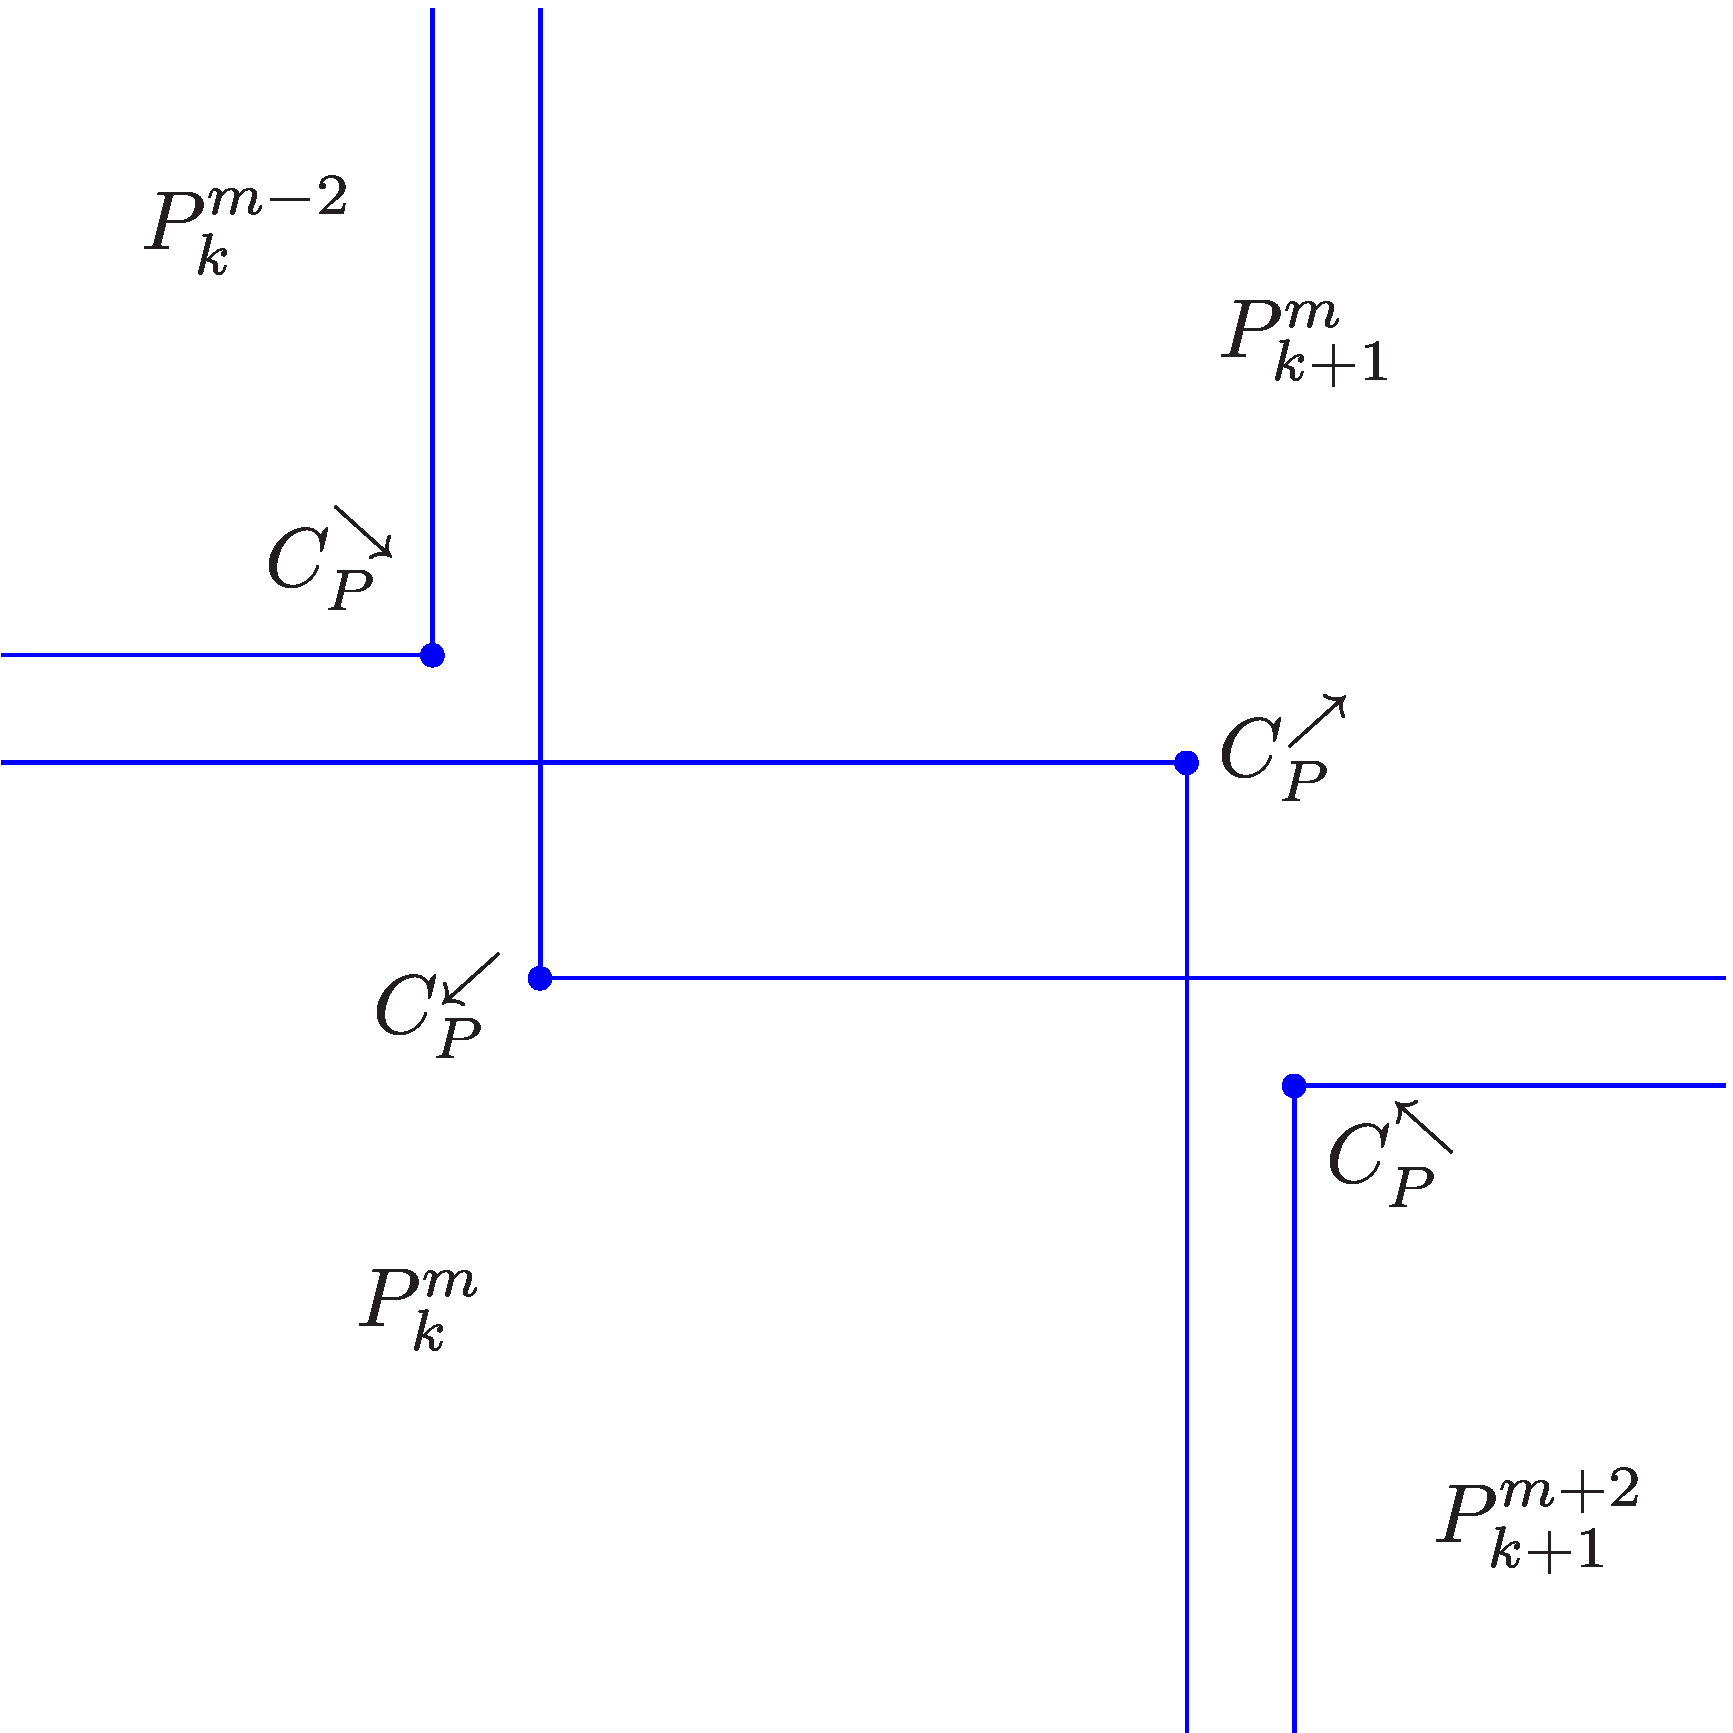
\includegraphics[width=.4 \textwidth]{../Figures/7/7.9e/result.png}
		\label{fig:add.change.schema.e}
	}
	\caption[Schematics of the boundaries of parameter regions associated with different symbolic sequences during the transition of the archetypal model to increasing branches]{
		Schematics of the boundaries of parameter regions associated with different symbolic sequences during the transition of the archetypal model to increasing branches.
		The boundaries of ``type A'' parameter regions are shown in blue while the boundaries of ``type B'' parameter regions are shown in red.
		Significant points where boundaries meet or cross are marked with dots.
	}
	\label{fig:add.change.schema}
\end{figure}

\Cref{fig:add.change.schema} shows multiple schematics that are used in this section to summarize all changes.
All schematics show some boundaries of the ``type A'' parameter regions $P^m_k, P^{m-2}_{k-1}, P^m_{k+1},$ and $P^{m+2}_{k+1}$ and all boundaries of the ``type B'' parameter region $Q^m_k$.
The ``type B'' parameter region is in-between all the ``type A'' parameter regions in the beginning.
This is shown in \Cref{fig:add.change.schema.a}.
The corners of the parameter regions are marked as follows.
The upper right corner of the ``type B'' parameter region in the middle is marked with the point $C_Q^\nearrow$.
Similarly, the lower right corner is marked with the point $C_Q^\searrow$ and the remaining corners with the points $C_Q^\nwarrow$ and $C_Q^\nwarrow$.
The corners of the ``type A'' parameter regions are marked analogously with $C_P^\nearrow, C_P^\searrow, C_P^\nwarrow,$ and $C_P^\swarrow$.
But here, the corners belong to different parameter regions.

The changes are summarized in the order they happen to the parameter regions that are considered in the previous sections.
This order might differ for different parameter regions.

First, the upper left corner $C_Q^\nwarrow$ of the lower right ``type A'' parameter region $P^{m+2}_{k+1}$ moves down and crosses the lower boundary of the upper right ``type A'' parameter region $P^m_{k+1}$.
This is visible in \Cref{fig:add.change.schema.b}.
The point where the two boundaries of the horizontally neighboring ``type A'' parameter regions cross is marked as $C_{P \cap P}^\leftarrow$ because this point is now the only left corner point of the overlapping parameter region $P^{m+2}_{k+1} \cap P^{m}_{k+1}$.
For higher values of $b_L$, the point $C_Q^\nwarrow$ moves further down which causes the point where the boundaries cross to move right.
In \Cref{fig:add.change.schema.c}, this crossing point is not visible anymore, since it moved out of the domain of the picture.
In \Cref{fig:add.change.schema.d}, it is visible again, but on the left side of the schema.
Strictly speaking, this is not the same point but the left boundary of the overlapping parameter region $P^m_k \cap P^{m-2}_{k}$.
This point then collides with the corner point $C_P^\nearrow$ which then causes the two ``type A'' parameter regions to not overlap anymore.
This final scenario can be seen in \Cref{fig:add.change.schema.e}.
In the spaces that opened up between the vertically neighboring ``type A'' parameter regions, there are big hybrid parameter regions $\left[P^{m+2}_{k+1} \mid P^{m}_{k+1}\right]$ and $\left[P^m_k \mid P^{m-2}_k\right]$, respectively.
The hybrid parameter regions are not shown in the schematics but while the overlapping parameter regions have only three boundaries, they too only have three boundaries and are bounded to the right only by one codimension-2 point.
At this point, their upper and lower boundaries meet.

As we can see in the schematics, this change starts first and finishes last.
While the described process occurs, another change starts happening.
The points $C_P^\searrow$ and $C_Q^\nearrow$ move down while the points $C_Q\searrow$ and $C_P^\nearrow$ move up.
As soon as the point $C_P^\swarrow$ crosses the upper boundary of $P^m_k$, the ``type A'' parameter regions $P^m_k$ and $P^m_{k+1}$ start to overlap.
This overlapping region is bounded to the right only by the point where the horizontal boundaries of those two parameter regions cross.
This point is marked as $C_{P \cap P}^\rightarrow$ in \Cref{fig:add.change.schema.c}.
Also at some parameter values the corner points $C_Q^\nwarrow$ and $C_Q^\searrow$ of the ``type B'' parameter region $Q^m_k$ in the middle collide.
This creates a codimension-2 point that bounds the parameter region $Q^m_k$ to the left, hence it is marked as $C_Q^\leftarrow$.
Both these newly created corner points move right, as can be seen in \Cref{fig:add.change.schema.d}.
Finally, the corner point $C_{P \cap P}^\rightarrow$ collides with the corner point $C_P^\nearrow$ and the two horizontal boundaries of the ``type A'' parameter regions stop crossing.
The overlapping parameter region $P^m_k \cap P^m_{k+1}$ is now bounded by four boundaries, as can be seen in \Cref{fig:add.change.schema.e}.
And the corner point $C_Q^\leftarrow$ crosses the right boundary of the ``type B'' parameter region, destroying the ``type B'' parameter region.

While that change is happening, one more change takes place.
This change does not happen by two boundaries crossing at one point like the last two changes.
Instead, the numeric evidence suggests that it happens at once.
The corner point $C_P^\nwarrow$ crosses the right boundary of $P^m_k$ at the same time, the lower right corner point of $P^{m}_{k}$ which is not pictured here crosses the left boundary of $P^{m+2}_{k+1}$.
This lower corner point is not pictured, but the lower right corner point of $P^{m-2}_k$ is pictured and marked as $C_P^\searrow$.
Here, the equivalent happens for the horizontally neighboring ``type A'' parameter regions $P^{m-2}_k$ and $P^m_{k+1}$.
In \Cref{fig:add.change.schema.c}, the horizontally neighboring ``type A'' parameter regions overlap and in \Cref{fig:add.change.schema.d}, the parameter regions do not overlap.
Instead, there is now space in-between the horizontally neighboring ``type A'' parameter regions.
In this space there now is a big hybrid parameter region and \gls{pal} structures, similar to the vertically neighboring ``type A'' parameter regions.

\subsubsection{Observations}

The local minima on branches $f_\A$ and $f_\C$ seem to be important for the ``type B'' parameter regions.
That means, parameter regions with coexisting asymmetrical cycles with the \textbf{same} period.
At the same time, these minima seem to prevent period-adding structures.
It will be proven next that ``type B'' parameter regions are impossible with only increasing branches.

\begin{lemma}[Number and Positions of Points of two Cycles on an Increasing Branch]
	Let $f_\X$ be an increasing branch of some model function $f$.
	If two cycles $\sigma_1$ and $\sigma_b$ have points on this branch, there are two possibilities for the relative number of points and relative position of the points.
	\begin{enumerate}
		\item Both cycles have the same number of points on the branch $f_\X$.
		      Let the first point of $\sigma_1$ be to the left of the first point of $\sigma_2$ on this branch w.l.o.g.
		      Then the last point of $\sigma_1$ is also to the left of the last point of $\sigma_2$ on this branch.
		      \Cref{fig:add.change.increasing.a} illustrates this case.
		\item One cycle has one more point on the branch $f_\X$.
		      Let $\sigma_1$ be the cycle with more points on this branch w.l.o.g.
		      Then the first point of $\sigma_1$ is to the left of the first point of $\sigma_2$ on this branch and the last point of $\sigma_1$ is to the right of the last point of $\sigma_2$ on this branch.
		      \Cref{fig:add.change.increasing.b} illustrates this case.
	\end{enumerate}
	\label{lemma:add.num.pos.points.increasing}
\end{lemma}

\begin{figure}
	\centering
	\subfloat[Same number of points]{
		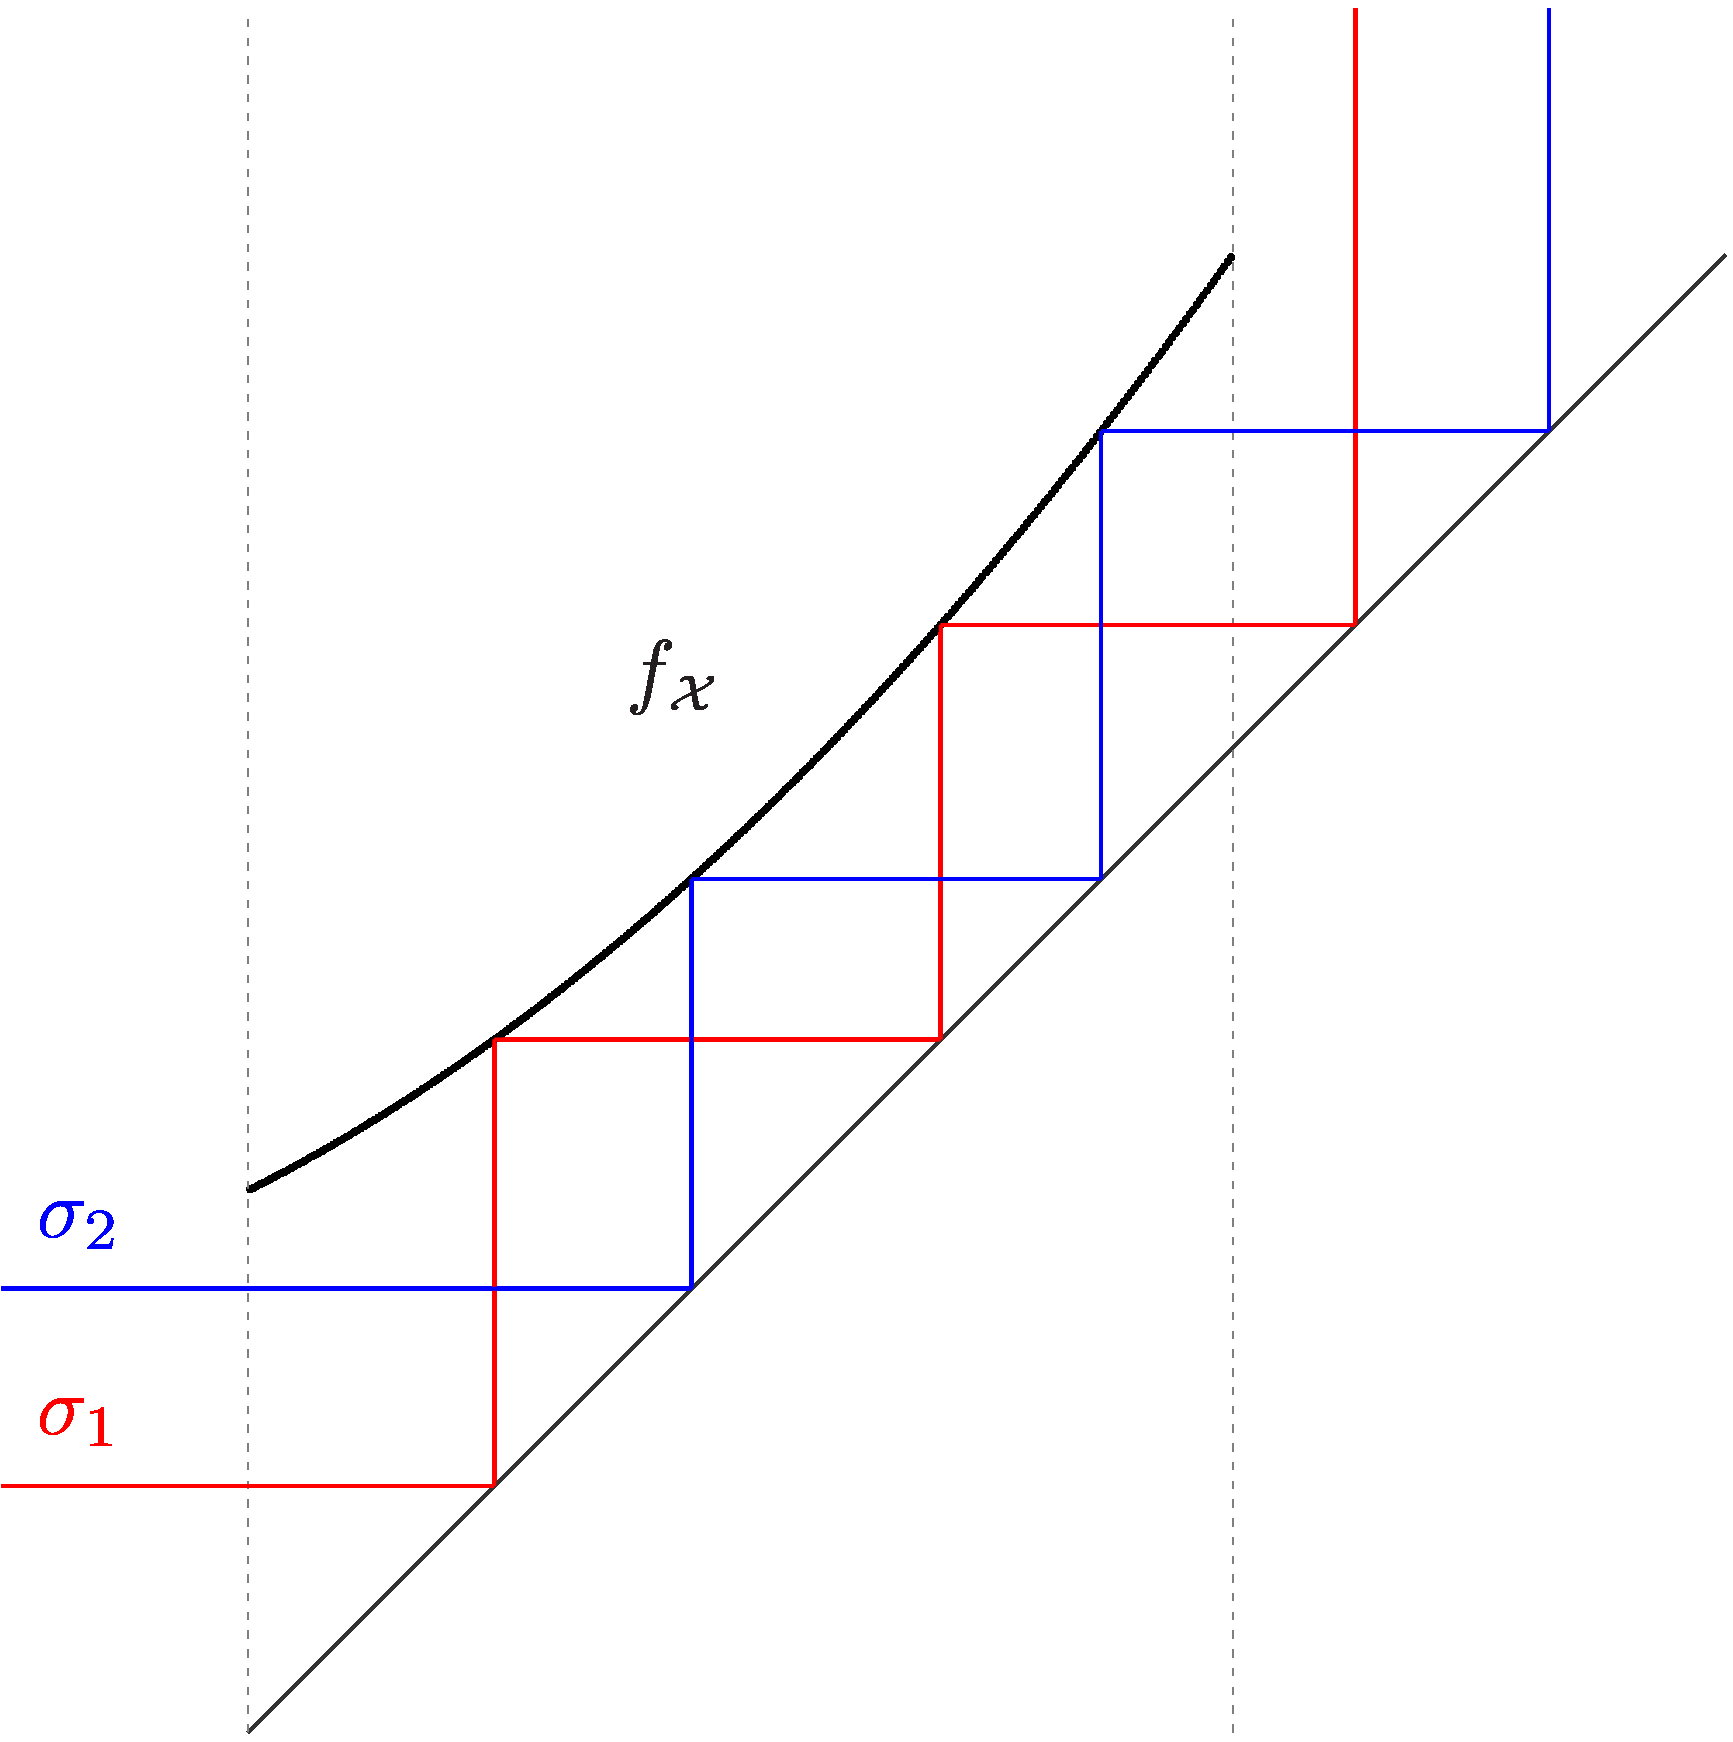
\includegraphics[width=.35 \textwidth]{../Figures/7/7.10a/result.png}
		\label{fig:add.change.increasing.a}
	} \quad
	\subfloat[Number of points differing by one]{
		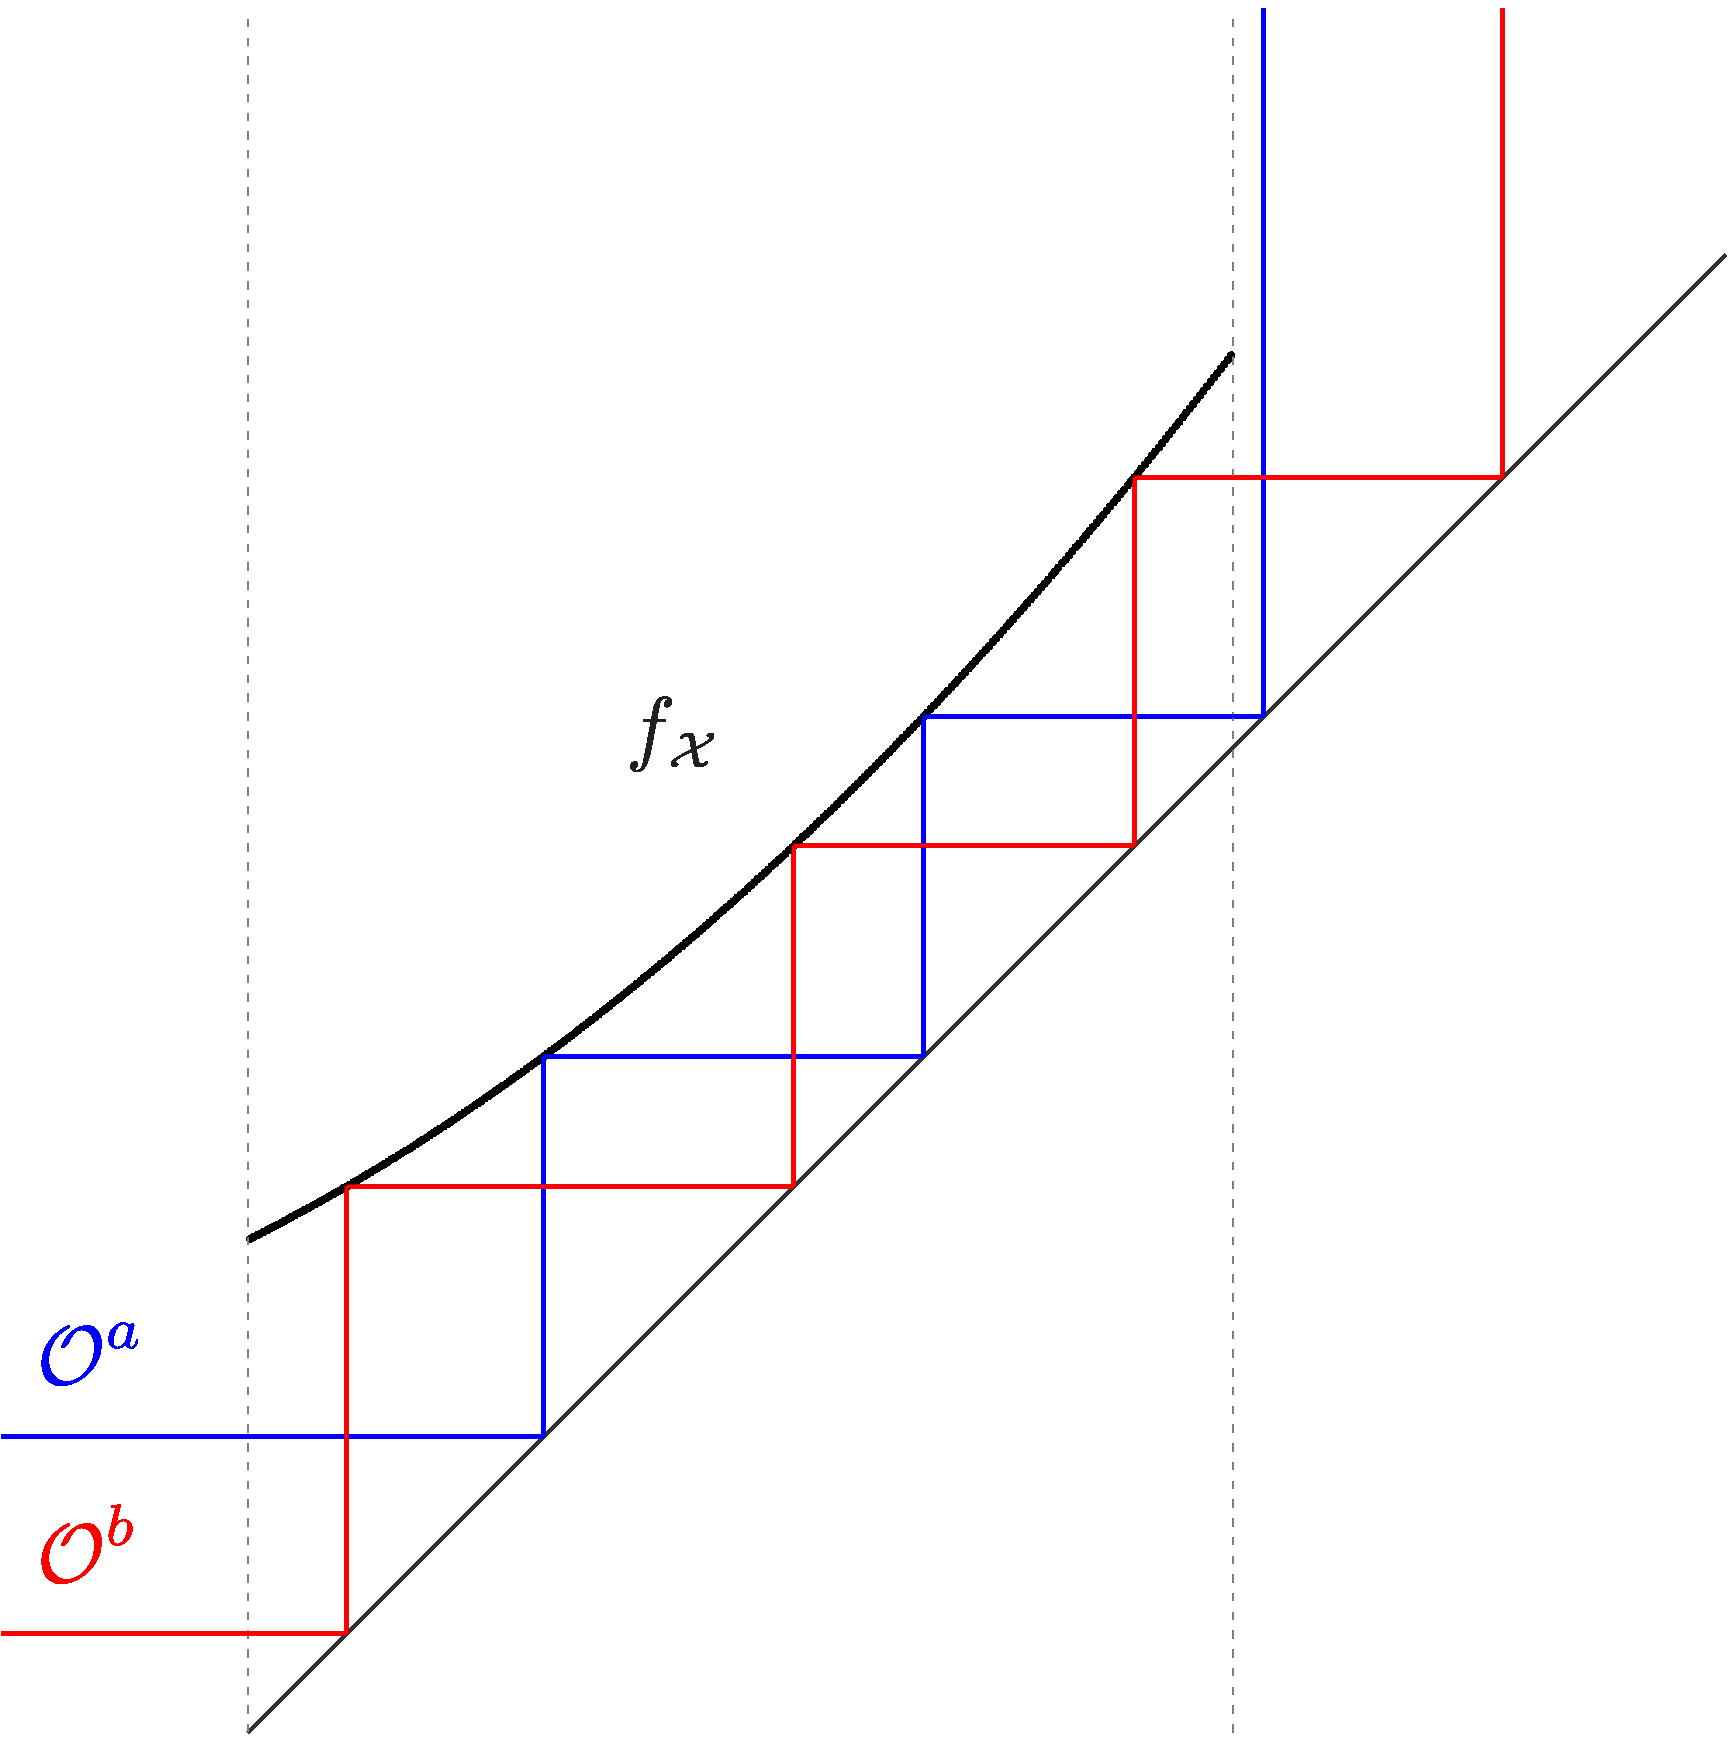
\includegraphics[width=.35 \textwidth]{../Figures/7/7.10b/result.png}
		\label{fig:add.change.increasing.b}
	}
	\caption[Illustration of the relative number and positions of the points of two cycles on an increasing branch]{
		Illustration of the relative number and positions of the points of two cycles on an increasing branch.
		Both figures show a function branch $f_\X$ and parts of two cycles, $\sigma_1$ shown in red and $\sigma_2$ shown in blue.
		(a) shows the case where both cycles have the same number of points on the branch $f_\X$ and the first point of $\sigma_1$ is to the left of the first point of $\sigma_2$ on this branch.
		(a) shows the case where the cycle $\sigma_1$ has one point more on the branch $f_\X$ than $\sigma_2$ and the first point of $\sigma_1$ is to the left of the first point of $\sigma_2$ on this branch.
	}
	\label{fig:add.change.increasing}
\end{figure}

\begin{theorem}[No ``Type B'' Parameter Regions with only Increasing Branches]
	The ``type B'' parameter regions are not possible in the increasing archetypal model.
	The minima on the branches $f_\A$ and $f_\C$ are essential for the bifurcation structure.
\end{theorem}

\begin{proof} \phantom{x} \\
	Let's assume that all branches of the archetypal model $f_\A, f_\B, f_\C,$ and $f_\D$ are increasing.
	And let $\sigma_1$ and $\sigma_2$ be ``type B'' twin cycles.
	The following conditions are true for such cycles.
	\begin{subequations}
		\begin{align}
			|\sigma_1|_\A - 1 & = |\sigma_2|_\A \label{equ:add.change.conseq.sigmaA} \\
			|\sigma_1|_\B + 1 & = |\sigma_2|_\B \label{equ:add.change.conseq.sigmaB} \\
			|\sigma_1|_\C + 1 & = |\sigma_2|_\C \label{equ:add.change.conseq.sigmaC} \\
			|\sigma_1|_\D - 1 & = |\sigma_2|_\D \label{equ:add.change.conseq.sigmaD}
		\end{align}
	\end{subequations}

	For \Cref{equ:add.change.conseq.sigmaA} to hold, the first point of  $\sigma_1$ needs to be to the left of first point of  $\sigma_2$ on the branch $f_\A$, because  $\sigma_1$ has one point more on this branch than  $\sigma_2$ and this branch is increasing.
	At the same time, the last point of  $\sigma_1$ must be to the right of the last point of  $\sigma_2$ on this branch.

	The order of the first points on the next branch, $f_\B$, is the same as for the last points on the branch $f_\A$.
	So the first point of  $\sigma_2$ is to the left of the first point of  $\sigma_1$ on this branch.
	For \Cref{equ:add.change.conseq.sigmaB} to hold, the last point of  $\sigma_2$ must be to the right of the last point of  $\sigma_1$ on this branch per the same logic as before.

	The order of the first points on the next branch, $f_\C$, is the same as for the last points on the branch $f_\B$.
	So the first point of  $\sigma_1$ is to the left of the first point of  $\sigma_2$ on this branch.
	This is a contradiction, since the first point of  $\sigma_1$ on the branch $f_\A$ is also to the left of the first point of  $\sigma_2$ on that branch.
	This violates the symmetry.
	Also, \Cref{equ:add.change.conseq.sigmaC} cannot be fulfilled if the first point of  $\sigma_1$ is to the left of the first point of  $\sigma_2$ on the branch $f_\C$, since the first point of  with more points, $\sigma_2$ in this case, on the branch must be to the left of the first point of the other cycle on that branch if the branch is increasing.

	\hfill $\blacksquare$
\end{proof}


\section{The Adding Structures}

We start by plotting the periods of stable cycles in a one-dimensional scan across a period-adding structure.
\Cref{fig:minrep.adding1.motivation.halved.1d.period.full} shows this scan, while \Cref{fig:minrep.adding1.corner.period.full} shows the period-structure.
The period range on the one-dimensional scan is marked in red between the regions $P_{10}^4$ and $P_{10}^4 \oplus P_9^4$.
The regions $P_{10}^4$ and $P_9^4$ have cycles as we expect, $\Cycle{\A^6\B^4\C^6\D^4}$ and $\Cycle{\A^5\B^4\C^5\D^4}$.
But the region $P_{10}^4 \oplus P_9^4$ is weirder.
In this region, there are two coexisting cycles, that act like the coexisting cycles in ``type B'' parameter regions.
They are hybrids of the cycles $P_{10}^4$ and $P_9^4$, $\Cycle{\A^6\B^4\C^5\D^4}$ and $\Cycle{\A^5\B^4\C^6\D^4}$, acting like one cycle on the one half of the model and acting like the other cycles on the other half.
This is the first sign, that there is something off about this period-adding structure.

Examining the one-dimensional scan of the period-adding structure, \Cref{fig:minrep.adding1.motivation.halved.1d.period.full}, closer we find some inconsistencies.
First, the period of the cycle $\sigma\rho$, 58, is larger than the periods of $\sigma$, 20, and $\rho$, 19, combined.
This is unexpected because the cycle $\sigma\rho$ should be the cycles $\sigma$ and $\rho$ glued together, and therefore its period should be exactly the sum of the periods of the cycles $\sigma$ and $\rho$.
Similarly, the period of $\sigma^2\rho$ should be the sum of the periods of $\sigma$ and $\sigma\rho$.
But instead, the period of $\sigma^2\rho$ is smaller than the period of $\sigma\rho$.
Is this not a period-adding cascade after all?

What is happening here is that a period-adding structure in the halved model manifests as this weird structure in the full model.
This becomes apparent when simulating the halved model in the same period ranges.
\Cref{fig:minrep.adding1.motivation.halved.1d.period.halved} shows the one-dimensional period scan in the halved model that corresponds to the scan in the full model in \Cref{fig:minrep.adding1.motivation.halved.1d.period.full}.
In the halved model, $\sigma$ is the cycle $\Cycle{\L^6\R^4}$, which is expected for the cycle $P_{10}^4$, and $\rho$ is the cycle $\Cycle{\L^6\R^4\L^5\R^4}$.
The cycle $\sigma\rho$ in between the two is now actually the two cycles glued together $\Cycle{(\L^6\R^4)^2\L^5R^4}$, as we would expect in a period-adding structure.
And its period is 29, which is the sum of the periods of the cycle $\sigma$, 10, and $\rho$, 19.

Now we can also see that the unusual hybrid cycles $P_{10}^4 \oplus P_9^4$ in the full model are the manifestation of the cycle $\Cycle{L^6\R^4\L^5\R^4}$ in the halved model.
This cycle is itself the first level of the real period-adding structure of the cycles $P_{10}^4$ and $P_9^4$, which are $\Cycle{\L^6\R^4}$ and $\Cycle{L^5\R^4}$ in the halved model.
\Cref{fig:minrep.adding1.large.adding} shows a one-dimensional scan of a full period-adding structure in the halved model at different parameter values that allow for larger period regions with higher periods, making them visible to us.
In the next section, we will explain what exactly the halved model is, why it works in our case, and how to translate symbolic sequences between it and the full model.

\begin{figure}
	\centering
	\subfloat[The full model]{
		\includegraphics[width=.4 \textwidth]{62_MinimalRepr_Adding/2D_Period_1_Zoomed/result.png}
		\label{fig:minrep.adding1.corner.period.full}
	}
	\subfloat[The halved model]{
		\includegraphics[width=.4 \textwidth]{63_MinimalRepr_Adding_Halved/2D_Period_1_Zoomed/result.png}
		\label{fig:minrep.adding1.corner.period.halved}
	}
	\caption{
		2D period scans of period-adding regions of the same model in two different versions.
		On the left, is the full version of the model and on the right, is the halved version of the model.
		The red markers between the regions $P_{10}^4$ and $P_{10}^4 \oplus P_9^4$ in both pictures, is the parameter range used for the 1D scans in \Cref{fig:minrep.adding1.motivation.halved.1d.period}.
	}
	\label{fig:minrep.adding1.corner.period}
\end{figure}

\begin{figure}
	\centering
	\subfloat[The full model]{
		\includegraphics[width=.4 \textwidth]{62_MinimalRepr_Adding/1D_Period_1_add_hor_D1/result.png}
		\label{fig:minrep.adding1.motivation.halved.1d.period.full}
	}
	\subfloat[The halved model]{
		\includegraphics[width=.4 \textwidth]{63_MinimalRepr_Adding_Halved/1D_Period_1_add_hor_D1/result.png}
		\label{fig:minrep.adding1.motivation.halved.1d.period.halved}
	}
	\caption{
		1D period scans of a period-adding cascade of the same model in two different versions.
		On the left, is the full version of the model and on the right, is the halved version of the model.
		The parameter range is the same in both models and is marked red in \Cref{fig:minrep.adding1.corner.period}.
	}
	\label{fig:minrep.adding1.motivation.halved.1d.period}
\end{figure}

\begin{figure}
	\centering
	\includegraphics[width=.7 \textwidth]{63_MinimalRepr_Adding_Halved/1D_Period_larger_adding/result.png}
	\caption{
		A 1D period scan of a horizontal adding structure at parameter values that allow us to see the adding more clearly.
		The fixed parameter values are $a_L = 1, b_L = 0.8, p_x = -0.39$ and $p_y$ is in the range $[0.082, 0.087]$.
		The cycles involved in the adding are $P_7^3$ and $P_7^2$.
	}
	\label{fig:minrep.adding1.large.adding}
\end{figure}

\begin{figure}
	\centering
	\includegraphics[width=\textwidth]{FareyTrees/Minrep_Adding1_Halved/adding.png}
	\caption{t}
	\label{fig:tree.adding1.hor.halved}
\end{figure}

\begin{figure}
	\centering
	\includegraphics[width=\textwidth]{FareyTrees/Minrep_Adding1_Full/adding.png}
	\caption{t}
	\label{fig:tree.adding1.hor.full}
\end{figure}

\subsection{The Halved Model}

The idea behind the halved model is that the model we have can be looked at in a different way than it was introduced in.
We know the model $m$ maps an input $x$ to $f(x) \mod 1$, meaning that if the output $f(x)$ is greater or equal to 1, we subtract 1 from it until it is in the range $[0, 1)$.
Similarly, we add 1 to it if it is smaller than 0 until it is in the desired range.
Now instead of confining the model to the domain of $[0, 1)$, we think of it repeating infinitely in both directions.
This proces is called lifting of circle maps and is described by \Citeauthor{devaney2021introduction} in his book~\cite{devaney2021introduction}.
We can achieve this by mapping $T^m: x \mapsto f(x - \lfloor x \rfloor)$.
This trick maps the input $x$ into the domain, on which our model function produces sensible results and causes it to repeat infinitely.
$T^m$ is now a lift of the model $m$ in the domain of all real numbers $\mathbb{R}$.
\Cref{fig:minrep.infinite.model.concept} illustrates this concept for the cycle $P_7^3$.
The blue square is the full model.
One can see, that the branch $f_\D$ is outside the blue square at its right edge.
This is because it was cut off and continued at the bottom of the square before, due to the $\mod 1$ operation.

\todo{this makes sense in the original problem domain}

In this model, there are no cycles that have multiple rotations.
Instead, the cycles that had multiple rotations in the full model, manifest as a sequence of different blocks of the full model.
Meaning for the example $P_7^3$, the same blocks of $\A^4\B^3\C^4\D^3$ are repeating infinitely.
But for an example with multiple rotations, such as $\A\B\C\D\A^2\B^2\C^2\D^2$, the blocks will not all be the same.
Instead, the blocks $\A\B\C\D$ and $\A^2\B^2\C^2\D^2$ will be alternating.

Now the symmetry of our function $f$ comes into play.
Since $f(x + 0.5) = f(x) + 0.5$ for $x \in [0, 0.5)$, we can split the infinite model into smaller blocks than the blue block of the full model.
The function of the infinite model repeats in blocks of size 0.5, these blocks are marked red in \Cref{fig:minrep.infinite.model.concept}.
These red blocks represent the halved model, it is the smallest repeating part of the infinite model $T^m$.
Basically we choose the smallest model, of which $T^m$ is a lift.
This happens to be exactly our model $m$ folded in half.
Se the halved model $h$ is defined on the interval $[0, \frac{1}{2})$ and maps $x \mapsto g(x) \mod \frac{1}{2}$, where $g(x)$ is the same as in our model $m$, defined in \Cref{sec:minrep.definition}.

To get the symbolic sequence of a cycle in the halved model, we look at the pattern in which different red blocks repeat along the infinite model.
For our example in the picture, there is only one red block that repeats infinitely, $\L^4\R^3$.
The next section will explain, how to translate cycles between the halved and full model.

\begin{figure}
	\centering
	\includegraphics[width=.7 \textwidth]{63_MinimalRepr_Adding_Halved/Cob_Vis_s/Manual/result.png}
	\caption{Illustration of the infinite model concept.}
	\label{fig:minrep.infinite.model.concept}
\end{figure}

\subsection{Translating Symbolic Sequences}

\subsubsection{Naive Algorithm}

Based on this concept of the infinite model, one can formulate a naive algorithm for translating symbolic sequences between the halved and full model.
We will start with the easier direction from the full to the halved model.
From this direction we can't learn much about the nature of the period-adding structure in the full model, the inverse will be more important for that.

To translate a symbolic sequence of the full model we start by writing it down.
For example $\A^4\B^3\C^4\D^3$.
Then we replace the symbols $\A$ and $\C$ by $\L$ and the symbols $\B$ and $\D$ by $\R$.
Now we have $\L^4\R^3\L^4\R^3$.
Finally, we have to check for redundancy in the resulting cycle.
In our example, the cycle $\L^4\R^3$ repeats twice in $\L^4\R^3\L^4\R^3$, so we just keep $\L^4\R^3$.
\todo{explain using the illustration}

The inverse is trickier.
We start by writing down the symbolic sequence in the halved model.
For example $h = \L^4\R^3\L4\R^3\L^3\R^3$.
Now we need to build pairs of rotations since each blue block fits two red blocks.
If there is one rotation left over at the end, we wrap around or equivalently write down the original sequence again.
We repeat this until we fit all rotations that we have written down.

\begin{lemma}
    \label{lemma:writing.down}
    For cycles in the halved model $h$ with an even number of rotations $n$, we only need to write the original cycle down once.
    For cycles in the halved model $h$ with an odd number of rotations $n$, we need to write the original cycle down exactly twice.
\end{lemma}

\begin{proof} \phantom{x}
    \begin{enumerate}
        \item Let $n = 2i$. Then, we can build $i$ pairs of rotations and fit all $2i$ rotations of the original model.
        \item Let $n = 2i + 1$. We start by building $i$ pairs of rotations, fitting $2i$ rotations.
              This will leave the last rotation unpaired o we write down the sequence of $2i + 1$ rotations again.
              Now we can pair up the last rotation of the first sequence we wrote down with the first rotation of the sequence we just wrote down.
              $2i$ rotations remain, which we can fit into $i$ pairs.
    \end{enumerate}
\end{proof}

Notice, our example symbolic sequence has 3 rotations.
This means we have to write down the original sequence twice $h^2 = \L^4\R^3\L4\R^3\L^3\R^3\L^4\R^3\L4\R^3\L^3\R^3$.

Then we pair up the rotations, this corresponds to drawing blue boxes around the red boxes in the infinite model.
In our example, we get the pairs $(\L^4\R^3\L^4\R^3)(\L^3\R^3\L^4\R^3)(\L^4\R^3\L^3\R^3)$.
The pairs then have to be translated using the function $t$ defined below.
The resulting symbolic sequence is $T(h) = \A^4\B^3\C^4\D^3\A^3\B^3\C^4\D^3\A^4\B^3\C^3\D^3$.

\begin{definition}
    The function $t$ maps two rotations of a symbolic sequence in the halved model to a single rotation in the full model.
    It is defined in the following way.
    \begin{align}
        t: & \L^a\R^b\L^c\R^d \mapsto \A^a\B^b\C^c\D^d
    \end{align}
\end{definition}

\begin{definition}
    The function $s$ shifts a symbolic sequence in the halved model by a single rotation.
    Let $\tau_1\tau_2 \dots \tau_n$ be a sequence in the halved model, where each $\tau_i$ is one rotation.
    Then $s$ is defined in the following way.
    \begin{align}
        s: & \tau_1\tau_2 \dots \tau_n \mapsto \tau_2 \dots \tau_n\tau_1
    \end{align}
    In the full model, there is a similar function, $s'$, that shifts a symbolic sequence in the full model by a single rotation.
    Let $\tau'_1\tau'_2 \dots \tau'_n$ be a sequence in the full model, where each $\tau'_i$ is one rotation.
    The $s'$ is defined in the following way.
    \begin{align}
        s': & \tau'_1\tau'_2 \dots \tau'_n \mapsto \tau'_2 \dots \tau'_n\tau'_1
    \end{align}
\end{definition}

\begin{definition}
    The two symbolic sequences $\sigma$ and $\rho$ in the full model are shift-equivalent $\sigma \equiv \rho$,
    if they both have the same number of rotations $n$
    and there is a number $0 \leq i < n$, such that $\sigma = s'^i(\rho)$.
    Where $s'^i$ is the same as applying $s'$ $i$ times.
\end{definition}

We need to repeat the whole process for each shift $s^i$ of the original symbolic sequence for $0 < i < n$ where $n$ is the number of rotations of the original symbolic sequence.
And we only keep the results that are not shift-equivalent to any previous result.
In our example, we would repeat the process for $s(h) = \L^4\R^3\L3\R^3\L^4\R^3$ and get the result $T(s(h)) = \A^4\B^3\C^3\D^3\A^4\B^3\C^4\D^3\A^3\B^3\C^4\D^3$.
This result is shift-equivalent to the first result by shifting it 2 times.
Last we need to repeat it for $s^2(h) = \L^3\R^3\L4\R^3\L^4\R^3$ and get the result $T(s^2(h)) = \A^3\B^3\C^4\D^3\A^4\B^3\C^3\D^3\A^4\B^3\C^4\D^3$.
This result is shift-equivalent to the first result by rotating it once.

Therefore the cycle $h$ in the halved model manifests as a single cycle $T(h)$ in the full model.
We write it as $F(h) = \{T(h)\} = \{\A^4\B^3\C^4\D^3\A^3\B^3\C^4\D^3\A^4\B^3\C^3\D^3\}$.
The result of $F$ is a set because the cycle $h$ in the halved model may manifest as multiple coexisting cycles in the full model.

\subsubsection{Insights}
\todo{better heading}

With this naive algorithm, we can start to investigate rules for the period-adding structure in the full model.

\begin{lemma}
    \label{lemma:equivalence.translations}
    The translations of the two cycles $h_1$ and $h_2 = r^{2i}(h_1)$ in the halved model are shift-equivalent $T(h_1) \equiv T(h_2)$ for all integers $i$.
\end{lemma}

\begin{proof}
    Let $h_1 = \tau_1\tau_2 \dots \tau_n$, therefore $h_2 = \tau_{2i+1} \dots \tau_n\tau_1 \dots \tau_{2i}$.
    The translations are $T(h_1) = t(\tau_1\tau_2)t(\tau_3\tau_4) \dots t(\tau_{n-1}\tau_n)$
    and $T(h_2) = t(\tau_{2i+1}\tau_{2i+2}) \dots t(\tau_{n-1}\tau_n)t(\tau_1\tau_2) \dots t(\tau_{2i-i}\tau_{2i})$.
    We can see that $T(h_2) = s'^i(T(h_1))$ and therefore $T(h_1) \equiv T(h_2)$.
\end{proof}

\begin{theorem}
    \label{theorem:coexistence.even}
    The mainfestations of a cycle in the halfed model $h$ is either $F(h) = \{T(h), T(s(h))\}$ or $F(h) = \{T(h)\}$.
    And \begin{enumerate}
        \item $F(h) = \{T(h), T(s(h))\}$ if the number of rotations of the sequence $h$ is even.
        \item $F(h) = \{T(h)\}$ if the number of rotations of the sequence $h$ is odd.
    \end{enumerate}
\end{theorem}

\begin{proof}
    Let $h = \tau_1\tau_2 \dots \tau_n$ a symbolic sequence in the halved model with $n$ rotations.
    We know from \Cref{lemma:equivalence.translations} that the only possible candidates for $F(h)$ are $T(h)$ and $T(s(h))$.
    These are the first two possibilities we check in the algorithm and all other shifts $T(s^i(h))$ with $2 \leq i < n$ are shift-equivalent to $T(h)$ or $T(s(h))$.
    So, in the following, we will only check for the shift-equivalence of these two candidates.
    \begin{enumerate}
        \item Let $n = 2i$.
              From \Cref{lemma:writing.down} we know that we only need to write down the original cycle $h$ once and thus we get the following translations.
              \begin{align*}
                          & T(h) = t(\tau_1\tau_2) t(\tau_3\tau_4) \dots t(\tau_{n-1}\tau_n) \\
                  \nequiv & T(h) = t(\tau_2\tau_3) t(\tau_4\tau_5) \dots t(\tau_n\tau_1)
              \end{align*}
              The two candidates are not shift-equivalent because the pair $t(\tau_1\tau_2)$ in $T(h)$ is not included in the other candidate $t(s(h))$.
              The same is true for any other pair, and therefore $F(h) = \{T(h), T(s(h))\}$.
        \item Let $n = 2i + 1$.
              From \Cref{lemma:writing.down} we know that we need to write down the original cycle $h$ exactly twice and thus we get the following translations.
              \begin{align*}
                         & T(h) = t(\tau_1\tau_2) t(\tau_3\tau_4) \dots t(\tau_n\tau_1) t(\tau_2\tau_3) \dots t(\tau_{n-1}\tau_n) \\
                  \equiv & T(h) = t(\tau_2\tau_3) \dots t(\tau_{n-1}\tau_n) t(\tau_1\tau_2) t(\tau_3\tau_4) \dots t(\tau_n\tau_1)
              \end{align*}
              The two candidates are shift-equivalent.
              By shifting the second candidate $T(s(h))$ $2i$ times, we get the first candidate $T(h)$.
              Therefore, the second candidate is discarded and $F(h) = \{T(h)\}$.
    \end{enumerate}
\end{proof}

Note that a result of $F(h) = \{T(h), T(s(h))\}$ means that the cycle in the halved model $h$ manifests as two coexisting cycles in the full model.

\subsubsection{Revised Algorithm}

With all these properties and functions we now can formulate a more compact algorithm, \Cref{alg:halved.to.full}, for translating symbolic sequences from the halved model into the full model.
This revised algorithm will be used in the following to explain the rules of the period-adding structure in the full model.

\begin{algorithm}
    \caption{Translating a Symbolic Sequence from the Halved Model to the Full Model}\label{alg:halved.to.full}
    \begin{algorithmic}
        \Require $h = \tau_1\tau_2 \dots \tau_n$ with $n > 0$
        \If{$n$ is even}
        \State \Return $\{t(\tau_1\tau_2) t(\tau_3\tau_4) \dots t(\tau_{n-1}\tau_n), t(\tau_2\tau_3) t(\tau_4\tau_5) \dots t(\tau_n\tau_1)\}$
        \ElsIf{$n$ is odd}
        \State \Return $\{t(\tau_1\tau_2) \dots t(\tau_{n}\tau_1) \dots t(\tau_{n-1}\tau_n)\}$
        \EndIf
    \end{algorithmic}
\end{algorithm}

\Cref{alg:full.to.halved} shows the inverse algorithm for translating symbolic sequences from the full model to the halved model for completeness.
It uses the inverse $t^{-1}$ of the function $t$.

\begin{definition}
    The function $t^{-1}$ maps one rotation of a symbolic sequence in the full model to two rotations in the halved model.
    It is defined in the following way.
    \begin{align}
        t^{-1}: & \A^a\B^b\C^c\D^d \mapsto \L^a\R^b\L^c\R^d
    \end{align}
\end{definition}

\begin{algorithm}
    \caption{Translating a Symbolic Sequence from the Full Model to the Halved Model}\label{alg:full.to.halved}
    \begin{algorithmic}
        \Require $f = \tau'_1\tau'_2 \dots \tau'_n$ with $n > 0$
        \State $d \gets t^{-1}(\tau'_1)t^{-1}(\tau'_2) \dots t^{-1}(\tau'_n) = \tau_1\tau_2 \dots \tau_m$
        \Comment $m = 2n$ is even
        \State $h \gets \tau_1\tau_2 \dots \tau_{\frac{m}{2}}$
        \If{$d = h^2$}
        \State \Return $h$
        \ElsIf{$d \neq h^2$}
        \State \Return $d$
        \EndIf
    \end{algorithmic}
\end{algorithm}

\subsection{Properties of the Period-adding Structure in the Full Model}

With this knowledge, we now can explain, why some cycles in the full model have a much lower period than expected in period-adding structures.

\begin{lemma}[$t$ Preserves Period]
    \label{lemma:t.preserves.period}
    The function $t$ preserves the period. $|\sigma_1\sigma_2| = |t(\sigma_1\sigma_2)|$.
\end{lemma}

\begin{proof}
    Let $\sigma_1\sigma_2 = \L^a\R^b\L^c\R^d$.
    \begin{align*}
        |\sigma_1\sigma_2| =  |\L^a\R^b\L^c\R^d|
        = a + b + c + d
        = |\A^a\B^b\C^c\D^d|
        = |t(\L^a\R^b\L^c\R^d)|
        = |t(\sigma_1\sigma_2)|
    \end{align*}
\end{proof}

\begin{theorem}[Period of Cycles in the Full Model]
    \begin{enumerate}
        \item If a cycle in the halved model manifests as two coexisting cycles in the full model, the period of either cycle is the same as the period of the cycle in the halved model. $|T(\sigma)| = |T(s_2(\sigma))| = |\sigma|$.
        \item If a cycle in the halved model manifests as a single cycle in the full model, the period of this cycle is double the period of the cycle in the halved model. $|T(\sigma)| = 2 |\sigma|$.
    \end{enumerate}
\end{theorem}

\begin{proof} \phantom{x}
    \begin{enumerate}
        \item From \Cref{theorem:coexistence.even} we know that if the cycle $\sigma$ in the halved model manifests as two coexisting cycles in the full model, $\sigma$ has an even number of rotations $n$.
              And its translation is $T(\sigma) = t(\sigma_1\sigma_2) t(\sigma_3\sigma_4) \dots t(\sigma_{n-1}\sigma_n)$.
              Combining this with the fact, that $t$ preserves the period of its input as described in \Cref{lemma:t.preserves.period}, we can calculate the period of $T(h)$ in the following way.
              \begin{align*}
                  |T(h)| & = |t(\sigma_1\sigma_2) t(\sigma_3\sigma_4) \dots t(\sigma_{n-1}\sigma_n)|           \\
                         & = |t(\sigma_1\sigma_2)| + |t(\sigma_3\sigma_4)| + \dots + |t(\sigma_{n-1}\sigma_n)| \\
                         & = |\sigma_1\sigma_2| + |\sigma_3\sigma_4| + \dots + |\sigma_{n-1}\sigma_n|          \\
                         & = |\sigma_1\sigma_2 \dots \sigma_n| = |h|
              \end{align*}
              So the period of the cycle $T(\sigma)$ in the full model is the same as the period of the cycle $\sigma$ in the halved model.
              The same calculation can be done for $T(s(\sigma))$ and is omitted here.
        \item Similarly we know that if the cycle $\sigma$ in the halved model manifests as a single cycle in the full model, $\sigma$ has an odd number of rotations $n$.
              And its translation is $T(\sigma) = t(\sigma_1\sigma_2) \dots t(\sigma_n\sigma_1) \dots t(\sigma_{n-1}\sigma_n)$.
              Its period can be calculated in the following way.
              \begin{align*}
                  |T(h)| & = |t(\sigma_1\sigma_2) \dots t(\sigma_n\sigma_1) \dots t(\sigma_{n-1}\sigma_n)|                      \\
                         & = |t(\sigma_1\sigma_2)| + \dots + |t(\sigma_n\sigma_1)| + \dots + |t(\sigma_{n-1}\sigma_n)|          \\
                         & = |\sigma_1\sigma_2| + \dots + |\sigma_n\sigma_1| + \dots + |\sigma_{n-1}\sigma_n|                   \\
                         & = |\sigma_1\sigma_2 \dots \sigma_n\sigma_1 \dots \sigma_{n-1}\sigma_n| = |\sigma\sigma| = 2 |\sigma|
              \end{align*}
              So the period of the cycle $T(\sigma)$ in the full model is twice the period of the cycle $\sigma$ in the halved model.
    \end{enumerate}
\end{proof}

\subsubsection{Rules for Combining Symbolic Sequences}

Looking at the farey tree in \Cref{fig:tree.adding1.hor.full}, we can see some regularities in the distribution of coexisting (yellow) and single (white) cycles in the full model.
These can be explained with \Cref{theorem:coexistence.even}.
\todo{last case not possible in our adding structures. proof!}
The third case in \Cref{theorem:child.coexistence} can't be seen in the farey tree but it follows from the proof of the first two cases.

\begin{theorem}[Multiplicity of Cycles Associated With Child Nodes Based on the Multiplicity of Cycles Associated With its Parent Nodes]
    \label{theorem:child.coexistence}
    \begin{enumerate}
        \item The child of a node with a single cycle and a node with two coexisting cycles has a single cycle.
        \item The child of two nodes with a single cycle has two coexisting cycles.
        \item The child of two nodes with two coexisting cycles, has two coexisting cycles.
    \end{enumerate}
\end{theorem}

\begin{proof} \phantom{x}
    \begin{enumerate}
        \item A node with a single cycle in the full model is the manifestation of a cycle with an odd number of rotations in the halved model.
              A node with two coexisting cycles in the full model is the manifestation of a cycle with an even number of rotations in the halved model.
              Their child is the manifestation of the two cycles in the halved model glued together.
              This glued-together cycle has an odd number of rotations and therefore manifests as a single cycle in the full model.
        \item Analogously, two cycles with an odd number of rotations glued together have an even number of rotations.
              Therefore, this glued-together cycle manifests as two coexisting cycles in the full model.
        \item Analogously, two cycles with an even number of rotations glued together have an even number of rotations.
              Therefore this glued-together cycle manifests as two coexisting cycles in the full model.
    \end{enumerate}
\end{proof}

Furthermore, we can formulate rules for the cycles in the child node of two nodes in the period-adding structure in the full model.

\begin{definition}[Merging two 4-syllables]
    The operation $\left[\phi_i \mid \psi_j\right]$ merges the two 4-symmables $\phi_i$ and $\psi_j$.
    Let $\phi_i = \A^a\B^b\C^c\D^d$ and $\psi_j = \A^e\B^f\C^g\D^h$.
    Then $\left[\phi_i \mid \psi_j\right] = \A^a\B^b\C^g\D^h$.
    It concatenates the first 2-syllable of $\phi_i$ with the second 2-syllable of $\psi_j$.
\end{definition}

\begin{theorem}[The Cycles of a Child Node of a Node With a Singular Cycle and a Node With 2 Coexisting Cycles]
    The child node of a node with a singular cycle $\phi = \phi_1\phi_2 \dots \phi_n$ and a node with two coexisting cycles $\phi^a = \phi^a_1\phi^a_2 \dots \phi^a_m$ and $\phi^b_1\phi^b_2 \dots \phi^b_m$ will have one of the following cycles.
    \begin{enumerate}
        \item If $\phi$ is associated with the left parent.
              \begin{align*}
                  \phi_1 \dots \phi_{\frac{n-1}{2}} \left[\phi_{\frac{n+1}{2}} \mid \phi^b_m\right]
                  \phi^b_1 \dots \phi^b_{m-1} \left[\phi^b_m \mid \phi_{\frac{n+1}{2}}\right]
                  \phi_{\frac{n+3}{2}} \dots \phi_n \phi^a
              \end{align*}
        \item If $\phi$ is associated with the right parent.
              \begin{align*}
                  \phi^a \phi_1 \dots \phi_{\frac{n-1}{2}} \left[\phi_{\frac{n+1}{2}} \mid \phi^b_m\right]
                  \phi^b_1 \dots \phi^b_{m-1} \left[\phi^b_m \mid \phi_{\frac{n+1}{2}}\right]
                  \phi_{\frac{n+3}{2}} \dots \phi_n
              \end{align*}
              Which is shift-equivalent to the first case.
              But this distinction must be made to guarantee the correctness of cycles in subsequent child nodes.
    \end{enumerate}
\end{theorem}

\begin{proof} \phantom{x}
    \begin{enumerate}
        \item Let $\sigma = \sigma_1\sigma_2 \dots \sigma_i$ with odd $i$ and $\rho = \rho_1\rho_2 \dots \rho_j$ with even $j$ and $T(\sigma) = \phi, T(\rho) = \psi^a$, and $T(s_2(\rho)) = \psi^b$.
              The child of both nodes in the halved model will have the cycle $\sigma\rho = \sigma_1\sigma_2 \dots \sigma_i \rho_1\rho_2 \dots \rho_j$.
              This will manifest as the following cycle in the full model.
              \begin{align*}
                  T(\sigma\rho) & = T(\sigma_1 \dots \sigma_i \rho_1 \dots \rho_j)                                                                              \\
                                & =
                  t(\sigma_1\sigma_2) \dots t(\sigma_i \rho_1) \dots t(\rho_j \sigma_1) \dots t(\sigma_{i-1}\sigma_i) t(\rho_1\rho_2) \dots t(\rho_{j-1}\rho_j) \\
                                & = \phi_1 \dots \phi_{\frac{n-1}{2}} t(\sigma_i \rho_1)
                  \psi^b_1 \dots \rho^b_{m-1} t(\rho_j \sigma_1)
                  \phi_{\frac{n+3}{2}} \dots \phi_n
                  \psi^a_1 \dots \psi^a_m                                                                                                                       \\
                                & =
                  \phi_1 \dots \sigma_{\frac{n-1}{2}} \left[\sigma_{\frac{n+1}{2}} \mid \rho^b_m\right]
                  \psi^b_1 \dots \psi^b_{m-1} \left[\rho^b_m \mid \sigma_{\frac{n+1}{2}}\right]
                  \phi_{\frac{n+3}{2}} \dots \phi_n
                  \psi^a                                                                                                                                        \\
              \end{align*}
        \item Let $\sigma = \sigma_1\sigma_2 \dots \sigma_i$ with even $i$ and $\rho = \rho_1\rho_2 \dots \rho_j$ with odd $j$ and $T(\sigma) = \psi^a, T(s_2(\sigma)) = \psi^b$, and $T(\rho) = \phi$.
              The child of both nodes in the halved model will have the cycle $\sigma\rho = \sigma_1l_2 \dots \sigma_i \rho_1\rho_2 \dots \rho_j$.
              This will manifest as the following cycle in the full model.
              \begin{align*}
                  T(\sigma\rho) & = T(\sigma_1 \dots \sigma_i \rho_1 \dots \rho_j)                                                                                             \\
                                & =
                  t(\sigma_1\sigma_2) \dots t(\sigma_{i-1}\sigma_i) t(\rho_1\rho_2) \dots t(\rho_j \sigma_1) \dots t(\sigma_i\rho_1) \dots t(\rho_j\sigma_1) \dots t(\sigma_i) \\
                                & =
                  \psi^a_1 \dots \psi^a_m
                  \phi_1 \dots \phi_{\frac{n-1}{2}} t(\sigma_i \rho_1)
                  \psi^b_1 \dots \psi^b_{m-1} t(\rho_j \sigma_1)
                  \phi_{\frac{n+3}{2}} \dots \phi_n                                                                                                                            \\
                                & =
                  \psi^a
                  \phi_1 \dots \phi_{\frac{n-1}{2}} \left[\phi_{\frac{n+1}{2}} \mid \psi^b_m\right]
                  \psi^b_1 \dots \psi^b_{m-1} \left[\psi^b_m \mid \phi_{\frac{n+1}{2}}\right]
                  \phi_{\frac{n+3}{2}} \dots \phi_n                                                                                                                            \\
              \end{align*}
    \end{enumerate}
\end{proof}

\begin{theorem}
    The child node of two nodes with a singular cycle, $\phi = \phi_1 \dots \phi_n$ and $\psi = \psi_1 \dots \psi_m$ respectively, has the following two cycles.
    \begin{align*}
        \phi_1 \dots \phi_{\frac{n-1}{2}} \left[\phi_{\frac{n+1}{2}} \mid \psi_{\frac{m+1}{2}}\right] \psi_{\frac{m+3}{2}} \dots \psi_m
    \end{align*}
    and
    \begin{align*}
        \phi_{\frac{n+3}{2}} \dots \phi_n \psi_1 \dots \psi_{\frac{m-1}{2}} \left[\psi_{\frac{m+1}{2}} \mid \phi_{\frac{n+1}{2}}\right]
    \end{align*}
\end{theorem}

\begin{proof}
    Let $\sigma = \sigma_1\sigma_2 \dots \sigma_i$ with odd $i$ and $\rho = \rho_1\rho_2 \dots \rho_j$ with odd $j$ and $T(\sigma) = \phi$ and $T(\rho) = \psi$.
    The child of both nodes in the halved model will have the cycle $\sigma\rho = \sigma_1 \dots \sigma_i \rho_1 \dots \rho_j$.
    This will manifest as the following two cycles in the full model.
    \begin{align*}
        T(\sigma\rho) & = T(\sigma_1 \dots \sigma_i \rho_1 \dots \rho_j)                                                                                  \\
                      & = t(\sigma_1\sigma_2) \dots t(\sigma_i\rho_1) \dots t(\rho_{j-1}\rho_j)                                                           \\
                      & = \phi_1 \dots \phi_{\frac{n-1}{2}} t(\sigma_i\rho_1) \psi_{\frac{m+3}{2}} \dots \psi_j                                           \\
                      & = \phi_1 \dots \phi_{\frac{n-1}{2}} \left[\phi_{\frac{n+1}{2}} \mid \psi_{\frac{m+1}{2}}\right] \psi_{\frac{m+3}{2}} \dots \psi_j
    \end{align*}
    and
    \begin{align*}
        T(s(\sigma\rho)) & = T(\sigma_2 \dots \sigma_i \rho_1 \dots \rho_j \sigma_1)                                                                         \\
                         & = t(\sigma_2\sigma_3) \dots t(\sigma_{i-1}\sigma_i) t(\rho_1\rho_2) \dots t(\rho_j\sigma_1)                                       \\
                         & = \phi_{\frac{n+3}{2}} \dots \phi_n \psi_1 \dots \psi_{\frac{m-1}{2}} t(\rho_j\sigma_1)                                           \\
                         & = \phi_{\frac{n+3}{2}} \dots \phi_n \psi_1 \dots \psi_{\frac{m-1}{2}} \left[\psi_{\frac{m+1}{2}} \mid \phi_{\frac{n+1}{2}}\right]
    \end{align*}
\end{proof}

\todo{last case not possible in our adding structures. proof!}

As mentioned before, the next case does not appear in the fare tree in \Cref{fig:tree.adding1.hor.full}.
But we will include it here for completeness.

\begin{theorem}
    The child node of two nodes with two coexisting cycles each, $\{\phi^a, \phi^b\}$ and $\{\phi^a, \phi^b\}$ respectively, has the following two cycles.
    \begin{align*}
        \phi^a\phi^a \qquad \text{and} \qquad
        \phi^b_1 \dots \phi^b_{n-1} \left[\phi^b_n \mid \phi^b_m\right] \phi^b_1 \dots \phi^b_{m-1} \left[\phi^b_m \mid \phi^b_n\right]
    \end{align*}
\end{theorem}

\begin{proof}
    Let $\sigma = \sigma_1 \dots \sigma_i$ with even $i$ and $\rho = \rho_1 \dots \rho_j$ with even $j$ and $T(\sigma) = \phi^a, T(s_2(\sigma)) = \phi^b, T(\rho) = \phi^a$, and $T(s_2(\rho)) = \phi^b$.
    The child of both nodes in the halved model will have the cycle $\sigma\rho$.
    This will manifest as the following two cycles in the full model.
    \begin{align*}
        T(\sigma\rho) & = T(\sigma_1 \dots \sigma_i \rho_1 \dots \rho_j) = t(\sigma_1\sigma_2) \dots t(\sigma_{i-i}\sigma_i) t(\rho_1\rho_2) \dots t(\rho_{j-1}\rho_j) \\
                      & = \phi^a_1 \dots \phi^a_n \phi^a_1 \dots \phi^a_m = \phi^a\phi^a
    \end{align*}
    and
    \begin{align*}
        T(s(\sigma\rho)) & = T(\sigma_2 \dots \sigma_i \rho_1 \dots \rho_j \sigma_1) = t(\sigma_2\sigma_3) \dots t(\sigma_i\rho_1) \dots t(\rho_j\sigma_1)   \\
                         & = \phi^b_1 \dots \phi^b_{n-1} t(\sigma_i\rho_1) \phi^b_1 \dots \phi^b_{m-1} t(\rho_j\sigma_1)                                     \\
                         & = \phi^b_1 \dots \phi^b_{n-1} \left[\phi^b_n \mid \phi^b_m\right] \phi^b_1 \dots \phi^b_{m-1} \left[\phi^b_m \mid \phi^b_n\right]
    \end{align*}
\end{proof}
\subsubsection{Rules for Combining Rotation-like Numbers}

\begin{figure}
    \centering
    \includegraphics[width=.8 \textwidth]{FareyTrees/Minrep_Adding1_Full_RotNum/adding.png}
    \caption{Farey tree with rotation numbers}
\end{figure}

\begin{definition}[Rotation-like Numbers]
    Rotation-like numbers for symbolic sequences $\sigma$ in the full model.
    \begin{align*}
        \rho_\A(\sigma) = \dfrac{|\sigma|_\A}{|\sigma|}, \quad
        \rho_\B(\sigma) = \dfrac{|\sigma|_\B}{|\sigma|}, \quad
        \rho_\C(\sigma) = \dfrac{|\sigma|_\C}{|\sigma|}, \quad
        \rho_\D(\sigma) = \dfrac{|\sigma|_\D}{|\sigma|}
    \end{align*}
    Where $|\sigma|_\A$ is the number of symbols $\A$ in the sequence.
    Analogous for the symbols $\B$, $\C$, and $\D$.
\end{definition}

\begin{definition}[Farey Addition]
    \todo{define}
\end{definition}

\begin{theorem}
    The child node of a node with a singular cycle $\sigma$ and a node with two coexisting cycles $\varrho^a$ and $\varrho^b$ will have the following rotation-like numbers.
    We will call the cycle associated with the child node $\pi$ in the following.
    \begin{align*}
        \rho_\A(\pi) & =
        \rho_\A(\sigma) \oplus \rho_\A(\varrho^a) \oplus \rho_A(\varrho^b) \\
        \rho_\B(\pi) & =
        \rho_\B(\sigma) \oplus \rho_\B(\varrho^a) \oplus \rho_B(\varrho^b) \\
        \rho_\C(\pi) & =
        \rho_\C(\sigma) \oplus \rho_\C(\varrho^a) \oplus \rho_C(\varrho^b) \\
        \rho_\D(\pi) & =
        \rho_\D(\sigma) \oplus \rho_\D(\varrho^a) \oplus \rho_D(\varrho^b)
    \end{align*}
    \todo{volle schreibweise überall?}
\end{theorem}

\begin{proof}
    \todo{prove}
\end{proof}

\begin{theorem}
    The child node of two nodes with a singular cycle, $\sigma$ and $\varrho$ respectively, will have the following period.
    We will call the two cycles associated with the child node $\pi^a$ and $\pi^b$ in the following.
    \begin{align*}
        |\pi^a| = |\pi^b| & = \dfrac{|\sigma| + |\varrho|}{2} = |\pi|
    \end{align*}
    And its rotation-like numbers will be the following.
    \begin{align*}
        \rho_\A(\pi^a) & = \dfrac{|\sigma_1 \dots \sigma_{\frac{n+1}{2}}|_\A + |\varrho_{\frac{m+3}{2}} \dots \varrho_m|_\A}{|\pi|} \\
        \rho_\B(\pi^a) & = \dfrac{|\sigma_1 \dots \sigma_{\frac{n+1}{2}}|_\B + |\varrho_{\frac{m+3}{2}} \dots \varrho_m|_\B}{|\pi|} \\
        \rho_\C(\pi^a) & = \dfrac{|\sigma_1 \dots \sigma_{\frac{n-1}{2}}|_\C + |\varrho_{\frac{m+1}{2}} \dots \varrho_m|_\C}{|\pi|} \\
        \rho_\D(\pi^a) & = \dfrac{|\sigma_1 \dots \sigma_{\frac{n-1}{2}}|_\D + |\varrho_{\frac{m+1}{2}} \dots \varrho_m|_\D}{|\pi|} \\
        \rho_\A(\pi^b) & = \dfrac{|\varrho_1 \dots \varrho_{\frac{m+1}{2}}|_\A + |\sigma_{\frac{n+3}{2}} \dots \sigma_n|_\A}{|\pi|} \\
        \rho_\B(\pi^b) & = \dfrac{|\varrho_1 \dots \varrho_{\frac{m+1}{2}}|_\B + |\sigma_{\frac{n+3}{2}} \dots \sigma_n|_\B}{|\pi|} \\
        \rho_\C(\pi^b) & = \dfrac{|\varrho_1 \dots \varrho_{\frac{m-1}{2}}|_\C + |\sigma_{\frac{n+1}{2}} \dots \sigma_n|_\C}{|\pi|} \\
        \rho_\D(\pi^b) & = \dfrac{|\varrho_1 \dots \varrho_{\frac{m-1}{2}}|_\D + |\sigma_{\frac{n+1}{2}} \dots \sigma_n|_\D}{|\pi|}
    \end{align*}
\end{theorem}

\begin{proof} \phantom{x}
    \begin{enumerate}
        \item \todo{prove period}
        \item \todo{prove rotation-like numbers}
    \end{enumerate}
\end{proof}

\todo{last case not possible in our adding structures. proof!}

\begin{theorem}
    The child node of two nodes with two coexisting cycles, $\{\sigma^a, \sigma^b\}$ and $\{\varrho^a, \varrho^b\}$ respectively, will have the following rotation-like numbers.
    We will call the two cycles associated with the child node $\pi^a$ and $\pi^b$ in the following.
    \begin{align*}
        \rho_\A(\pi^a) & = \rho_\A(\sigma^a) \oplus \rho_\A(\varrho^a) \\
        \rho_\B(\pi^a) & = \rho_\A(\sigma^a) \oplus \rho_\A(\varrho^a) \\
        \rho_\C(\pi^a) & = \rho_\A(\sigma^a) \oplus \rho_\A(\varrho^a) \\
        \rho_\D(\pi^a) & = \rho_\A(\sigma^a) \oplus \rho_\A(\varrho^a) \\
        \rho_\A(\pi^b) & = \rho_\A(\sigma^b) \oplus \rho_\A(\varrho^b) \\
        \rho_\B(\pi^b) & = \rho_\A(\sigma^b) \oplus \rho_\A(\varrho^b) \\
        \rho_\C(\pi^b) & = \rho_\A(\sigma^b) \oplus \rho_\A(\varrho^b) \\
        \rho_\D(\pi^b) & = \rho_\A(\sigma^b) \oplus \rho_\A(\varrho^b)
    \end{align*}
\end{theorem}

\begin{proof}
    \todo{prove}
\end{proof}

In the usual case with two symbols, the rotation numbers are monotone.
In our case, this is not true when considering both rotation-like numbers of coexisting cycles.
The first step is a counter example, $\dfrac{6}{19} > \dfrac{6}{20}$ and $\dfrac{6}{19} > \dfrac{5}{18}$.
But when considering the farey sum of the rotation-like numbers of coexisting cycles, the monotony holds.

\begin{theorem}{Monotony of Rotation-like Numbers in the Full Model}
    The rotation-like numbers for one symbol are monotone in the farey tree of a period-adding structure in the full model, when considering the farey sum of the rotation-like numbers of coexisting cycles.
    \todo{sentences too long and complicated in enumeration}
    \begin{enumerate}
        \item The rotation-like numbers that correspond to the cycle of a child node of a parent node with a singular cycle and a parent node of two coexisting cycles, is in between the corresponding rotation-like number of the parent node with a singular cycle and the corresponding sum of rotation-like numbers of the parent node with two coexisting cycles.
              \begin{align*}
                       & \rho_X(\sigma) < \rho_X(\pi) < \rho_X(\varrho^a) \oplus \rho_X(\varrho^b) \\
                  \lor & \rho_X(\sigma) > \rho_X(\pi) > \rho_X(\varrho^a) \oplus \rho_X(\varrho^b)
              \end{align*}
        \item The farey sum of the rotation-like numbers that correspond to each coexisting cycle of a child node of two nodes with a singular cycle each, is in between the corresponding rotation-like numbers of the parent nodes.
              \begin{align*}
                       & \rho_X(\sigma) < \rho_X(\pi^a) \oplus \rho_X(\pi^b) < \rho_X(\varrho) \\
                  \lor & \rho_X(\sigma) > \rho_X(\pi^a) \oplus \rho_X(\pi^b) > \rho_X(\varrho)
              \end{align*}
    \end{enumerate}
\end{theorem}

\begin{proof}
    \todo{prove}
\end{proof}
